\newpage
{\bfseries ҒТАМР 50.43.15}

{\bfseries ЖОЛ ҚИЫЛЫСТАРЫНДАҒЫ КӨЛІК ҚҰРАЛДАРЫНЫҢ АҒЫНЫН НАҚТЫ УАҚЫТ
РЕЖИМІНДЕ ДИНАМИКАЛЫҚ РЕТТЕУ}

{\bfseries \textsuperscript{1}Д.С. Жамангарин, \textsuperscript{1}С.А.
Алтынбек, \textsuperscript{1}А.Д. Тулегулов\textsuperscript{🖂},}

{\bfseries \textsuperscript{1}К.М. Акишев, \textsuperscript{2}Н.П.
Сапарходжаев}

\textsuperscript{1}Қ. Құлажанов атындағы Қазақ технология және бизнес
университеті, Астана, Қазақстан,

\textsuperscript{2}Д. Серікбаев атындағы Шығыс Қазақстан техникалық
университеті., Өскемен, Қазақстан

\textsuperscript{🖂}Корреспондент-автор: tad62@ya.ru

Соңғы жылдары қалалық жерлерде бағдаршамдардың өткізу қабілеттілігін
арттыру мақсатында көлік құралдарының кептелісін динамикалық басқаруға
көбірек көңіл бөлінуде. Осы мақсатта кіру жылдамдығына негізделген жеке
traf C шамдары үшін бірқатар адаптивті басқару алгоритмдері ұсынылды.
Алайда, нақты уақыт режимінде бірнеше қиылыстардан өтетін жол
жағдайларын ескере отырып, бағдаршамдардың өткізу қабілеттілігін арттыру
мәселесіне көңіл бөлінді. Бұл жұмыста біз әр түрлі шығыс бағыттарына
кіретін көліктерді қарастыра отырып, максималды өткізу мәселені
тұжырымдаймыз. Содан кейін біз жаңа адаптивті traf C жарық сигналын
басқару алгоритмін ұсынамыз, ол жол қозғалысын барынша арттыруға және
қиылыста көлік құралдарының күту уақытын қысқартуға мүмкіндік береді.
Ұсынылған алгоритм негізгі және көршілес қиылыстардың нақты уақыттағы
жол жағдайына байланысты traf C жарық сигналының фазалары мен ұзақтығын
реттейді. SUMO модельдеу арқылы біз ұсынылған алгоритмнің өткізу
қабілеттілігі мен орташа жүру уақыты тұрғысынан тиімділігін көрсетеміз.

{\bfseries Түйін сөздер:} адаптивті жүйелер, traf C, адаптивті басқару,
алгоритм, SUMO модельдеу.

{\bfseries ДИНАМИЧЕСКОЕ РЕГУЛИРОВАНИЕ ПОТОКА ТРАНСПОРТНЫХ СРЕДСТВ НА
ПЕРЕКРЕСТКАХ В РЕЖИМЕ РЕАЛЬНОГО ВРЕМЕНИ}

{\bfseries \textsuperscript{1}Д.С. Жамангарин, \textsuperscript{1}С.А.
Алтынбек, \textsuperscript{1}А.Д.
Тулегулов}\textsuperscript{🖂}{\bfseries ,}

{\bfseries \textsuperscript{1}К.М. Акишев, \textsuperscript{2}Н.П.
Сапарходжаев}

\textsuperscript{1}Казахский университет технологии и бизнеса имени К.
Кулажанова, Астана, Казахстан,

\textsuperscript{2}Восточно-Казахстанский технический университет им. Д.
Серикбаева,

Усть-Каменогорск, Казахстан,

e-mail: tad62@ya.ru

В последние годы все больше внимания уделяется динамическому управлению
заторами транспортных средств с целью увеличения пропускной способности
светофоров в городских районах. С этой целью был предложен ряд
алгоритмов адаптивного управления для отдельных ламп traf C, основанных
на скорости входа. Однако с учетом дорожных условий, проходящих через
несколько перекрестков в режиме реального времени, внимание было уделено
вопросу увеличения пропускной способности светофоров. В данной статье мы
формулируем проблему максимальной пропускной способности, рассматривая
транспортные средства, въезжающие в разные направления. Затем мы
представляем новый адаптивный алгоритм управления световым сигналом traf
C, который позволяет максимизировать дорожное движение и сократить время
ожидания транспортных средств на перекрестке. Предлагаемый алгоритм
регулирует фазы и продолжительность светового сигнала traf C в
зависимости от дорожной ситуации в реальном времени между основным и
соседним пересечениями. С помощью моделирования SUMO мы демонстрируем
эффективность предложенного алгоритма с точки зрения пропускной
способности и среднего времени в пути

{\bfseries Ключевые слова}. адаптивные системы, traf C, адаптивное
управление, алгоритм, моделирование SUMO.

{\bfseries DYNAMIC CONTROL OF THE FLOW OF VEHICLES AT INTERSECTIONS IN REAL
TIME}

{\bfseries \textsuperscript{1}D. Zhamangarin, \textsuperscript{1}S.
Altynbek, \textsuperscript{1}A. Tulegulov}\textsuperscript{🖂}{\bfseries ,
\textsuperscript{1}K. Akishev, \textsuperscript{2}N. Saparkhodzhaev}

\textsuperscript{1}K. Kulazhanov Kazakh University of Technology and
Business, Astana, Kazakhstan

\textsuperscript{2}D. Serikbayev East Kazakhstan Technical University,
Ust-Kamenogorsk, Kazakhstan

e-mail: tad62@ya.ru

In recent years, more and more attention has been paid to dynamic
traffic congestion management in order to increase traffic light
capacity in urban areas. To this end, a number of adaptive control
algorithms have been proposed for individual traf C lamps based on the
input speed. However, taking into account the road conditions passing
through several intersections in real time, attention was paid to the
issue of increasing the traf C light capacity. In this article, we
formulate the problem of maximum throughput by considering vehicles
entering in different directions. Then we present a new adaptive traffic
light control algorithm that maximizes traf C and reduces the waiting
time for vehicles at the intersection. The proposed algorithm adjusts
the phases and duration of the traf C light signal depending on the
real-time road conditions of the main and adjacent intersections.
Through SUMO simulations, we demonstrate the effectiveness of the
proposed algorithm in terms of bandwidth and average travel time.

{\bfseries Key words.} adaptive systems, traf C, adaptive control,
algorithm, SUMO modeling.

{\bfseries Кіріспе.} Мегаполистерде урбанизацияға байланысты белгілі бір
жолдардағы автокөлік тығыздығы жоғары қарқынмен өсті. Бұл жолдың
кептелуіне, апаттарға, жанармай шығынына, СО шығарындыларына және
трафиктің кешігуіне әкелді {[}1,2{]}. Бұл мәселелер зерттеу жұмыстарының
назарын арттыруға түрткі болды және көлік қозғалысын басқарудың әртүрлі
стратегияларын әзірлеуге әкелді. Пайда болған стратегиялардың
бірі-қауіпсіздік камералары, traf C бейнекамералары, пьезоэлектрлік
датчиктер, индуктивті ілмектер және т.б. сияқты әртүрлі сенсорлық
технологияларды қолдану арқылы жиналған ақпаратқа сүйенетін
интеллектуалды көлік жүйесі ұғымын жүзеге асыру, жол жағдайын бақылау
және автокөлік жүргізушілерін сигналдары арқылы ескертуге болады.
Алайда, ITS-де қолданылатын бақылаудың мұндай әдеттегі әдістері шектеулі
қамту мен техникалық қызмет көрсетудің жоғары құнына байланысты тиімді
болмайды. Осы кемшіліктерді жою және нақты уақыт режимінде трафиктің
нақты деректерін жинау үшін ITS тұжырымдамасы сымсыз байланыс
технологияларымен толықтырылған, бұл көлік құралдарының арнайы желісінің
дамуына әкеледі. Сонымен қатар, traf C жарықтандыру уақытын жақсарту
үшін сымсыз сенсорлық желілер пайдаланылды {[}3,4{]}.

{\bfseries Материалдар мен әдістер.} Қалалық жолдардағы С қозғалысының
жағдайын жақсартуға арналған танымал VTM стратегияларын екі топқа бөлуге
болады. Бірінші топ traf C деректерін жинауға, пайдалануға және деректер
негізінде көліктерді айналып өтетін қайта бағыттау алгоритмдерін
қолдануға бағытталады {[}5,6{]}. Сонымен қатар, зерттеулер әрбір жолдың
нақты уақыттағы қозғалыс жағдайларын ескеруге мүмкіндік беру үшін сымсыз
байланыс технологиялары мен есептеу ресурстарындағы жетістіктерді
пайдалана отырып, traf C адаптивті басқаруды зерттейді {[}7,8{]}.
Зерттеу жұмыстарының көпшілігінің негізгі бағыты негізінен бір қиылысты
қиылыстыра отырып, traf C өткізу қабілетін арттыруға бағытталған; тек
бірнеше зерттеулер traf C максимизациясы үшін бірнеше қиылыстарды
қарастырады {[}9,10{]}. Алдыңғы жұмыстардан айырмашылығы, бұл жұмыс
мақсатты қиылыстағы және оның төрт бағыттағы көршілес қиылыстарындағы
нақты уақыттағы жағдайды ескере отырып, көлік құралдарының трафигін
максимизациялау мәселесін қарастырады және TFM - ді максималды бүтін сан
ретінде модельдейді.

Әдетте кептеліс тудыратын жол желісіне кіретін көлік құралдары әр түрлі
шығыс бағыттармен жүруге ниетті болғандықтан, кіру және шығу нүктелері
бірдей көлік құралдарының ағыны 0 және 1 желісіндегі геокартаға
түсірілуі мүмкін. Сонымен қатар, бір 0-ға жататын көлік құралдарының
саны, яғни шығу және келу позициялары бірдей көлік құралдары тобы
белгілі бір аралықтын сұранысына сәйкес келуі мүмкін. Біз жол желісін
gd(V;E) бағытталған графигі түрінде ұсынылған 0 желісіне геокартаға
түсіреміз, мұнда V және E сәйкесінше барлық қиылыстар мен жол
сегменттерін қамтиды. G-ге сүйене отырып, біз қарастырылған мәселесін
қуаттылық, 0 сигналдың уақыт үнемдеу және сұранысты қанағаттандыру
шарттарымен MCF-мен салыстыруға болатындығын көрсетеміз. Содан кейін біз
1-ші қиылысынан белгілі бір бағытқа қарай жасыл шамды күтіп тұрған
көліктерді ескере отырып, MCF үлгісін тұжырымдаймыз .

Қалыптасқан MCF мәселесін шешу үшін біз кептеліс пен бос жасыл ұзақтықты
азайту құралы ретінде бірнеше қиылыстардың(атомдардың) жол жағдайларын
ескеретін адаптивті traf C жарық фазасы мен ұзақтығын оңтайландыру
алгоритмін енгіземіз. Негізінде, traf C өткізу қабілеттілігін арттыруға
және қиылыста және оның қиылыстарында күту уақытын қысқартуға тырысады.
Сонымен қатар, трафиктің өткізу қабілеттілігінің артуы және күту
уақытының қысқаруы жергілікті және көршілес қиылыстардың айналасындағы
жолдардың қозғалыс деңгейін ескере отырып, динамикалық түрде реттеледі
және теңестіріледі. Traf C деректерін жинау үшін көлік құралдарындағы
борттық қондырғылар, Iare - дегі I жол бойындағы бөлімшелердегі (Rsu)
Obu және жол бойындағы қондырғылар (Rsu) арасындағы әртүрлі
коммуникациялық технологиялар пайдаланылады. Kіретін көліктердің саны,
барлық бағыттарды күту уақыты және т. б. сияқты i-дегі traf C
статистикасын бақылау.

Traf C деректері негізінде алынған кептеліс деңгейіне сүйене отырып,
өтіп бара жатқан көліктердің санын көбейту мен i - де орташа күту
уақытын қысқарту арасындағы тепе-теңдікті сақтау үшін traf C жарықты
басқарудың әртүрлі тәсілдерін қолданады.

Aвтокөлік туралы деректер негізінде алынған кептеліс деңгейіне сүйене
отырып, өтіп бара жатқан көліктердің санын көбейту мен i - де орташа
күту уақытын қысқарту арасындағы тепе-теңдікті сақтау үшін C
трафигіндегі жарықты басқарудың әртүрлі тәсілдерін қолданады. Tрафигінің
төмен көлемі байқалған кезде, күту уақытын қысқарту үшін бос жасыл
уақытты жоюға назар аударады. Сонымен қатар, С автокөліктің қарқынды
жағдайында назары жақын маңдағы жолдардағы кептелістерді азайтуға
бағытталған. Екі жағдайда да traf C жарық циклін реттеуді және/немесе
жергілікті және жақын маңдағы қиылыстардағы бақыланатын traf C деректері
негізінде жасыл жарық фазаларын және олардың ұзақтығын таңдау мен ретке
келтіруді оңтайландыруды таңдайды. Модельдеу нәтижесінде атомның
трафиктің өзгеруіне және өткізу қабілеттілігіне және пайдаланушының
кідірісіне бейімделудегі тиімділігі артады.

\emph{Aдаптивті бағдаршамды оңтайлату тәсілі}

АБОТ-тың басты ерекшелігі-жолдағы көлік құралдарының тығыздығының
динамикалық өзгеруіне байланысты traf c оңтайландырудың екі түрлі
тәсілін қолданылады. Тraf c жарық агентінен тұрады, атап айтқанда traf c
бақылаушысы және бағалаушы (TFW) және traf c жарық сигналын реттегіш
болады. Бағдаршам параллель жұмыс істейді және бір уақытта 1-суретте
көрсетілгендей бір-бірімен байланысады.

\begin{figure}[H]
	\centering
	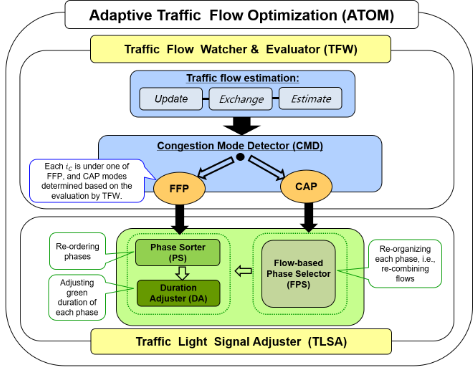
\includegraphics[width=0.8\textwidth]{assets/158}
	\caption*{}
\end{figure}

{\bfseries 1 --сурет. ЕКІ агент арасындағы өзара байланыс}

ATOM traf C жалпы өткізу қабілетін жақсартуды және i-де күтілетін
көліктің орташа өткізу қабілетін азайтуды таңдайды. АБОТ екі жұмыс
істейді, атап айтқанда TFW және TLSA.

TFW жергілікті және жақын маңындағы қиылыстардағы С трафигінің
динамикалық өзгерістерін бақылайды және i бағытында келе жатқан С
трафигінің көлемін, сондай-ақ i-ден шығатын жолдардағы жағдайларды
бағалайды. Деректерді жинауды жол датчиктері, 802.11 p, 802.16, яғни
WiMAX немесе LTE-V немесе 3gpp Cellular-V2X(C-V2X) сияқты ӘРТҮРЛІ V2V,
V2I және I2I технологияларын қолдану арқылы іс жүзінде жүзеге асыруға
болады. Содан кейін TFW бақыланатын жолдағы кептеліс деңгейін бағалайды.
Негізінде, tfw кептелу режимінің детекторы (CMD) i күйін екі режимге
жіктейді, атап айтқанда, бос 0 кезеңі (FFP) және үздіксіз реттелетін
кезең. Сонымен қатар, TFW жүргізетін traf c оңтайландыруының әсерін
мезгіл-мезгіл аңықтап және өнімділікті жақсарту үшін нәтижелерді TLSA-ға
қайтарады. Сонымен қатар, TLSA төменде түсіндірілгендей, TFW бағалаған
i-дегі кептеліс деңгейіне байланысты әртүрлі стратегияларды қолдану
арқылы бағдаршамды оңтайландырады.

Бұл i-де қалатын немесе өтетін көлік құралдарының жалпы көлемі аз
болатын уақыт кезеңін анықтап, осылайша i-дегі traf c өткізу
қабілеттілігі негізінен циклдің ұзақтығына әсер етеді, оның барысында
әрбір кем дегенде бір рет жасыл шамға ауысады. FFP-де, әдетте, i-ден әр
түрлі бағытта өтетін көліктердің орташа күту уақытын қысқарту үшін қысқа
циклға артықшылық беріледі, өйткені i қызмет көрсететін көліктердің
жалпы саны аз. Сондықтан, FFP кезінде TLSA, бұдан әрі TLSA деп
белгіленеді, traf c жарық циклінің сәйкес ұзындығын есептейді мен онда
барлық F бір рет жасыл шаммен сақталады және жасыл сигналдың реті мен
ұзақтығын салыстырмалы түрде көп кіретін бағыттарға қолайлы етіп
реттейді. Сонымен қатар, FFP цикл ұзақтығын, фазаларын және жасыл
жарықтың ұзақтығын кезең - кезеңімен реттеуге байланысты үш ішкі
деңгейге бөлінеді.

Уақыт сигналдары симуляция арқылы тексеріледі.

\emph{Симуляциялық орта және тиімділік көрсеткіштері}

Модельдеу Python тілінде SUMO көмегімен жүзеге асырылды {[}11,12{]}.
Эксперименттер қолданылған жол торын да, нақты жол желісін де
пайдаланады. Біріншісі жолдың әртүрлі ұзындығы мен енінде АБОТ
тиімділігін бағалауға мүмкіндік береді. 2(а) суретінен көрініп
тұрғандай, қарастырылатын тор 13 қиылыстан, кіру және шығу жолақтары
опциялары бар 44 жол сегментінен тұрады. Жолдың барлық учаскелерінің
ұзындығы бірдей. Сегмент ұзындығын өзгерту өткізу қабілетін, демек АБОТ
өнімділігін өзгертеді. Сонымен қатар, орташа қаланың нақты жол желісі
қарастырылады. 2(b)-(c) суреттерінде көрсетілгендей, жалпыға ортақ көше
карталары арқылы импортталады; Сәйкес параметрлер 1-кестеде келтірілген.
Басқаша айтқанда, АБОТ өнімділігі синтетикалық және нақты жол
желілерінің көмегімен тексеріледі (кесте 1).

{\bfseries 1 --кесте. Жол желісінің ақпараттары}

\begin{longtable}[]{@{}
  >{\raggedright\arraybackslash}p{(\columnwidth - 6\tabcolsep) * \real{0.4094}}
  >{\raggedright\arraybackslash}p{(\columnwidth - 6\tabcolsep) * \real{0.1509}}
  >{\raggedright\arraybackslash}p{(\columnwidth - 6\tabcolsep) * \real{0.1725}}
  >{\raggedright\arraybackslash}p{(\columnwidth - 6\tabcolsep) * \real{0.2672}}@{}}
\toprule\noalign{}
\begin{minipage}[b]{\linewidth}\raggedright
Параметр
\end{minipage} &
\multicolumn{2}{>{\raggedright\arraybackslash}p{(\columnwidth - 6\tabcolsep) * \real{0.3234} + 2\tabcolsep}}{%
\begin{minipage}[b]{\linewidth}\raggedright
Тор желісі
\end{minipage}} & \begin{minipage}[b]{\linewidth}\raggedright
Нақты жол желісі
\end{minipage} \\
\midrule\noalign{}
\endhead
\bottomrule\noalign{}
\endlastfoot
Жиектерінің жалпы саны &
\multicolumn{2}{>{\raggedright\arraybackslash}p{(\columnwidth - 6\tabcolsep) * \real{0.3234} + 2\tabcolsep}}{%
88} & 311 \\
Жолақтардың жалпы саны & 176 & 440 & 2172 \\
Жиек ұзындығы (м) & 200 & 800 & Әртүрлі {[}1,40{]} \\
Жолдың жалпы ұзындығы (м) & 17600 & 70400 & 10470 \\
Бағдаршам сигналдарының саны &
\multicolumn{2}{>{\raggedright\arraybackslash}p{(\columnwidth - 6\tabcolsep) * \real{0.3234} + 2\tabcolsep}}{%
13} & 137 \\
\end{longtable}

Біз топтық маршрутты таңдаудың екі әдістемесі негізінде зерттейміз, атап
айтқанда, ең қысқа жүру қашықтығы және Logit моделі {[}13{]}. АБОТ
өнімділігі \(i_{C}\) мақсатты қиылысында келесі төрт көрсеткіш арқылы
бағаланады:

\begin{itemize}
\item
  Қызмет көрсету мөлшерлемесі -- бұл желіні пайдалануға тырысқан жалпы
  көлік құралдарының ішіндегі жол желісіндегі көліктер санының қатынасы.
  Ол бағдаршамды басқару алгоритмдерінің негізгі өнімділігін көрсетеді.
  Неғұрлым тиімді байланыс алгоритмі қиылыстарда көбірек көліктерге
  қызмет көрсетеді және жоғары қызмет көрсету жылдамдығын береді.
\item
  Көлік құралдарының орташа күту уақыты (секунд): көлік құралдарының
  \(i_{C}\) -де орташа күту уақытының өлшемі. Күту уақыты неғұрлым қысқа
  болса, алгоритм соғұрлым жақсы жұмыс істейді. Ол \(i_{C}\) қиылысынан
  өтетін барлық көліктердің орташа сомасына тең.
\item
  Орташа қозғалыс жылдамдығы (км/сағ): желі арқылы жүруін аяқтайтын
  көлік құралдары үшін орташа қозғалыс жылдамдығына тең. Әрбір көліктің
  жылдамдығы оның жүру ұзақтығын жол жүру уақытына бөлу арқылы
  есептеледі.
\item
  Тоқтаған көліктердің орташа саны: \(i_{C}\) нүктесінде жасыл
  бағдаршамды күтуге тура келген көліктердің орташа санын білдіреді.
\item
  Желіде жүретін көліктердің жалпы саны: қанша көлік жүріп жатқанын
  көрсетеді және осылайша модельдеу уақыты бойынша желіде тұрады.
\end{itemize}

Жол жүруді аяқтаған көліктердің жалпы саны: желіден шыққан көліктер
санын хабарлайды. Ең дұрысы, барлық алгоритмдер және модельдеу уақыты
арқылы анықталатын бірдей мәнге жинақталуы керек, дегенмен уақыт
алгоритмнің тиімділігіне байланысты өзгереді

{\bfseries Нәтижелер мен талқылау.}

\emph{Симуляция нәтижелері}

Біз көліктің келу жылдамдығын өзгерту арқылы кептелістің бірнеше
деңгейін модельдейміз, мұнда μ {[}0.2, 3{]} аралығы таңдалады және көп
кептеліс желілерін имитациялау үшін басқа жол желісі конфигурациясына
байланысты өзгерді. Мысалы, жол сегментіне 2 жолағы бар желіде 0,5
секундқа орнатылады және осылайша 3600 секундтық модельдеу уақытында
конфигурацияланған жол желісіне барлығы 7200 көлік жүктеледі. Цикл
бастапқыда 12 фазадан тұрады және оның ұзақтығы 120 секундқа орнатылады;
демек, әрбір фазада 10 секунд бойы жасыл шам жанып тұрады. Модельдеу
нәтижелері SUMO жасаған жиынтық файлдан жиналады. Жеке эксперименттердің
нәтижелері 10 көліктен астам орташа бағаланады және осылайша барлық
нәтижелер 90\% интервалы талдауына байланысты үлгідегі орташа мәннің
10\% шегінде қалады.

\emph{Бір жолда 2 жолдағы тор желі}

2 суретте 2 жолақты тор желісіндегі алгоритмдердің өнімділігін 0,1
өсімімен 0,5 пен 1 \hspace{0pt}\hspace{0pt}аралығында өзгереді. 2(а)
суретінде АБОТ жол желісіндегі кептеліс деңгейіне қарамастан қызмет
көрсету деңгейі бойынша барлық базалық көрсеткіштерден асып түсетінін
көрсетеді. АБОТ ең кептеліс жолдарды құрайтын 0,5 көмегімен 45\% қызмет
көрсету деңгейіне жетеді.

\begin{figure}[H]
	\centering
	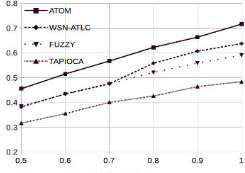
\includegraphics[width=0.8\textwidth]{assets/159}
	\caption*{}
\end{figure}
\begin{figure}[H]
	\centering
	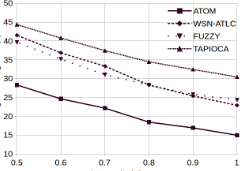
\includegraphics[width=0.8\textwidth]{assets/160}
	\caption*{}
\end{figure}

а) б)

\begin{figure}[H]
	\centering
	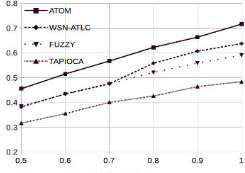
\includegraphics[width=0.8\textwidth]{assets/159}
	\caption*{}
\end{figure}
\begin{figure}[H]
	\centering
	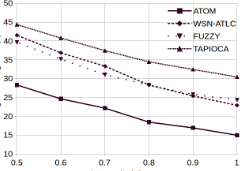
\includegraphics[width=0.8\textwidth]{assets/160}
	\caption*{}
\end{figure}

в) г)

{\bfseries 2-сурет. (а) қызмет көрсету жылдамдығы, (б) орташа күту уақыты,
(в) жасыл шамның жануын күту кезінде тоқтаған көліктердің орташа саны,
және (г) олардың қалыпты жүру жылдамдығы}

\emph{Бір жолға 5 жолақты желілік желі}

Біз жолдардың санын және әрбір жол сегментінің ұзындығын сәйкесінше 800
м-ге дейін ұлғайту арқылы электр желісін ұлғайттық. 3-суретте нәтижелер
көрсетілген. Осы қондырғыдағы жолдың ені мен ұзындығының ұлғаюын ескере
отырып, 2 жолақты тор желісіне ұқсайтын жол кептелісі деңгейлерін
модельдеу үшін 0,6-дан 1,4-ке дейін таңдалады. 2 жолақты желіге
қарағанда 5 жолақты желілік желіде қызмет көрсетудің жоғары
көрсеткіштерін көрсетеді. Өткізу қабілеттілігінің артуын ескере отырып,
тиімділігі фазаны салыстыру үшін екі жолақты таңдаудың шектелуіне
байланысты төмендейді, бұл оның кеңейтілген жол желісіндегі қызмет
көрсету жылдамдығын төмендетеді. Тұтастай алғанда, АБОТ осындай үлкен
жолды орнату үшін өнімділікті айтарлықтай жақсартады, базалық
көрсеткіштер бойынша салыстырғанда 0,6-дан 1,4-ке дейін өседі. 3(а)
суреттегі нәтижелер ІРІ жол желілері үшін АБОТ-тың масштабталуын
көрсетеді.

\begin{figure}[H]
	\centering
	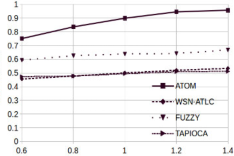
\includegraphics[width=0.8\textwidth]{assets/161}
	\caption*{}
\end{figure}\begin{figure}[H]
	\centering
	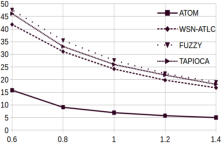
\includegraphics[width=0.8\textwidth]{assets/162}
	\caption*{}
\end{figure}

а) б)

\begin{figure}[H]
	\centering
	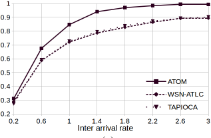
\includegraphics[width=0.8\textwidth]{assets/163}
	\caption*{}
\end{figure}
\begin{figure}[H]
	\centering
	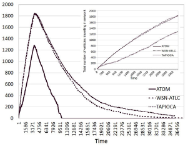
\includegraphics[width=0.8\textwidth]{assets/164}
	\caption*{}
\end{figure}

в) г)

{\bfseries 3-сурет. АБОТ өнімділігін бір жолға 5 жолақты желілік желіде
салыстыру (а) қызмет көрсету жылдамдығы, (б) орташа күту уақыты, (в)
тоқтатылған көліктердің орташа саны және (г) қалыпты жүргізу жылдамдығы}

Бағдаршамның бағытталған жұмысы сигнал беру уақытын анықтау кезінде бір
немесе бірнеше қиылыстар қарастырылатынына байланысты екі санатқа бөлуге
болады. Бір қиылысу үшін мақсат жасыл сигналды оңтайлы жоспарлау болып
табылады. Мысалы traf C жарық реттегіші қиылыста келе жатқан көліктердің
баратын соңғы нүктесі аңықталады; жасыл шамды жоспарлаудың екі
стратегиясы ұсынылады, атап айтқанда, орташа күту/жол жүру уақытын
қысқарту мақсатында межелі жерге дейінгі аз орташа қашықтық болады. Екі
тәсіл де негізінен нақты уақыт режиміндегі трафикке негізделген
қашықтықтың кешігуін азайтуға бағытталған. Сонымен қатар, бүкіл сапар
барысында аялдамалардың жалпы санын азайтуға және осылайша
шығарындыларын азайтуға бағытталған.

Мақалада traf C реттеу кезінде бірнеше көршілес бөлімдер қарастырылды.
Мысалы, ережеге негізделген вертикалды дайындалған, көршілес
қиылыстардың қозғалыс шамдары жергілікті деңгейде үйлестірілген. Жұмыс
кеңейтілген {[}11,12{]} аймақтық деңгейде қосымша иерархиялық
бақылаушы/контроллер компоненті ұсынылды. Сонымен қатар, traf C жарық
жүйелеріне көп агент негізіндегі алгоритмдер қолданылды {[}13{]}. IEEE
802.15.4 технологиясы мен динамикалық фазалары арқылы өзара байланысқан
және бұрылыстарды факторинг кезінде жасыл уақытты есептейтін бірнеше
анық емес логикалық контроллерлерді пайдалану жолдары анықталды. Тraf C
көлемінің өзгеруін бақылау үшін сенсорларды пайдаланады, соның негізінде
олар бөлінген көп агентті жүйені пайдаланып N\textsubscript{d} көлік
құралының жүру кезіндегі ең қысқа жасыл шамдар, қиылыстарда күту уақыты
бойынша азайтылады. Көп агентті арматураны оқыту алгоритмдері {[}14{]}
пайдаланып, мұнда жергілікті және жақын қиылыстардың реакциялары traf C
шамдарының уақытын реттеу үшін қарастырылады, бұл тәсілдер жоғары
есептеу күрделілігін қажет етіп қабылдайды.

Бұл мақалада біз нақты уақыт режимінде жиналған қозғалыс жағдайын ескере
отырып, мақсатты қиылыстағы бағдаршам шамдарын бақылау арқылы сигналдың
максималды жылдамдығын арттыруға тырыстық. Біз жол желісін gd (V; E)
бағытталған графигі арқылы желісі ретінде ұсынамыз, мұндағы V
қиылыстарды қамтиды, яғни, E жол сегменттерінен, яғни арасындағы
бағытталған жиектерден тұрады. G негізінде біз бақыланатын бағдаршамды
ұсынамыз.

Қиылыстағы көліктердің қозғалыс бағытын біле отырып, төрт бағыттың
әрқайсысынан i-ге қанша көлік кіретінін? Мысалы, 4(b) суретте
көрсетілген i-ге кіретін 12 көліктің ішінде жеті көлік i-ге қарай жүруі
керек деп болжануда.

\begin{figure}[H]
	\centering
	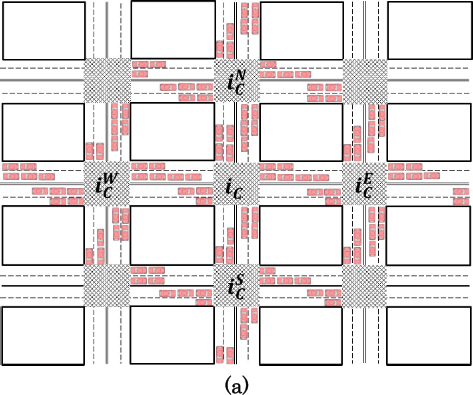
\includegraphics[width=0.8\textwidth]{assets/165}
	\caption*{}
\end{figure}

\begin{figure}[H]
	\centering
	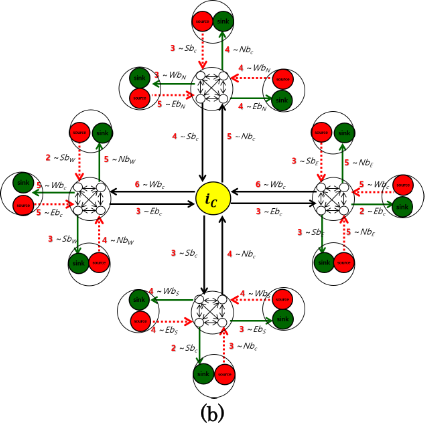
\includegraphics[width=0.8\textwidth]{assets/166}
	\caption*{}
\end{figure}

\begin{figure}[H]
	\centering
	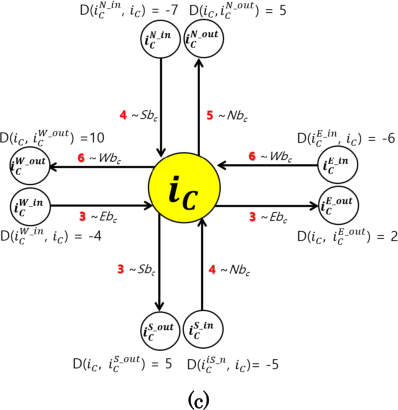
\includegraphics[width=0.8\textwidth]{assets/167}
	\caption*{}
\end{figure}

{\bfseries 4-сурет. Қиылыстағы көліктердің қозғалыс бағыттары}

TFM максималды бүтін санға дейін азайтылуы ағынының проблемасы шешіледі.
Оң жақ қиылыстағы қозғалыс ағынын бағытталған график түрінде ұсынылған
ағындық желіге салыстыруға болады. GD (V,E), V және E-қиылыстар
арасындағы қиылыстар мен жол сегменттерінің жиынтығы, тиісінше, (b)
тармағында көрсетіледі. (С) бөлігінде V-2-V кіретін Немесе шығатын
қозғалыс көлемі, Сондай-ақ әрбір 2 жол сегментінде жасыл шамды күтетін
қозғалыс көлемі қосымша көрсетіледі.

\emph{Зерттеу нәтижелерін талқылау.} Тraf C жарық фазасы мен ұзақтығын
реттеу арқылы i-ге байланысты көліктің жалпы Traf C көлемін барынша
арттыруға тырысады. Біз жаяу жүргіншілерді қарастырмайтындықтан,
оңтайландыру процедурасы жаяу жүргіншілердің i-де жолдарды кесіп өтуі
үшін ең аз жасыл уақытты есептемейді.

Сонымен қатар, автомобиль жүргізушілерге арналған көліктерді, сондай-ақ
өзін-өзі басқаратын көліктерді қарастырады; біріншісі үшін жеке көліктің
қозғалыс бағытын жүргізуші әр қиылыста, мысалы, v2i технологияларын
пайдалану арқылы немесе жүргізушінің ұялы телефонындағы қолданба арқылы
қамтамасыз етеді деп болжанады.

{\bfseries Қорытынды.} Бұл мақалада біз бағдаршам, жаңа traf c басқару
алгоритмін ұсындық. Адаптивті басқару әрбір қиылыста кіретін с уақыт
көлемі есептелінді, сонымен қатар көлік құралдарының әрбір уақыт үшін
келесі жол сегментінің кептеліс жағдайы тандалды. Содан кейін бағдаршам
traf c жарық фазаларын және олардың ұзақтығын көрші қиылыстармен бірлесе
отырып реттейді. Сонымен қатар, тәжірибеге үлестірілген немесе
орталықтандырылған түрде қолдануға болады. Нақты жол желілерін қолдана
отырып, ауқымды модельдеу тәжірибелері арқылы тексеріледі. Модельдеу
нәтижелері жол өткізу қабілеттілігін, көлік құралын күтудің орташа
уақытын және бәсекелес схемаға сәйкес көлік аялдамаларының орташа санын
жақсартатынын көрсетті. Негізінде, көбірек көліктердің жол желісі арқылы
өтуіне мүмкіндік береді және олардың жүру уақытын қысқартады, бұл тіпті
жоғары кептеліс жағдайында да көбірек көліктердің қозғалуына
көмектеседі. Осылайша, мұндай қондырғыдағы жолдың әртүрлі кептеліс
жағдайларында айқын өнімділігі оның тиімділігіне әсер етеді және іс
жүзінде тиімді екендігінің нақты дәлелі ретінде қарастырылады.

{\bfseries Әдебиеттер}

1. Бадагуев Б.Т. Эксплуатация транспортных средств (организация и
безопасность движения). -- М.: Альфа-Пресс, 2012. -- 240 с. ISBN
978-5-94280-556-2

2. Дудко Н.И., Петровец В.Р., Бершадский В.Ф. Безопасность движения
механических транспортных средств: пособие -- Горки: БГСХА, 2014. -- 237
с. ISBN 978-985-467-490-2

3. Блинкин М.Я. Безопасность дорожного движения: история вопроса,
международный опыт, базовые институции. -- М.: Изд. дом Высшей школы
экономики, 2013. -- 240 с. ISBN: 978-5-7598-1086-5

4. Волков В.С. Электрооборудование транспортных и
транспортно-технологических машин: учебное пособие -- М.: Академия,
2010. -- 208 с. ISBN 978-5-7695-5749-1

5. Горев, А. Э.Основы теории транспортных систем: учебное пособие / А.
Э. Горев; СПбГАСУ. -- СПб., 2010. -- 214 с. ISBN 978-5-9227-0266-9

6. Майборода М.Е., Беднарский В.В. Грузовые автомобильные перевозки. --
М.: Феникс, 2008. -- 442 с. ISBN 978-5-222-14364-3

7. Клинковштейн Г.И. Организация дорожного движения: учебник для вузов.
-- 5-е изд., перераб. и доп. -- М: Транспорт, 2001 -- 247. ISBN
9785277022405

8. Урыков В.А., Зеленина Л.И. Модели транспортного инфраструктурного
комплекса // https://web.snauka.ru/issues/2014. 18.06.2020.

9. Морозов И.И. и др. Численное исследование транспортных потоков на
основе гидродинамических моделей // Компьютерные исследования и
моделирование. -- 2011. -- Т. 3, №4. -- С. 389-412.

10. Буслаев А.П., Новиков А.В., Приходько В.М. и др. Вероятностные и
имитационные подходы к оптимизации автодорожного движения. -- М.: Мир,
2003. -- 368 с. ISBN 9785030036465

{\bfseries References}

1. Badaguev B.T. Jekspluatacija transportnyh sredstv (organizacija i
bezopasnost\textquotesingle{} dvizhenija). -- M.:
Al\textquotesingle fa-Press, 2012. -- 240 s. ISBN 978-5-94280-556-2
{[}in Russian{]}

2. Dudko N.I., Petrovec V.R., Bershadskij V.F.
Bezopasnost\textquotesingle{} dvizhenija mehanicheskih transportnyh
sredstv: posobie -- Gorki: BGSHA, 2014. -- 237 s. ISBN 978-985-467-490-2
{[}in Russian{]}

3. Blinkin M.Ja. Bezopasnost\textquotesingle{} dorozhnogo dvizhenija:
istorija voprosa, mezhdunarodnyj opyt, bazovye institucii. -- M.: Izd.
dom Vysshej shkoly jekonomiki, 2013. -- 240 s. ISBN: 978-5-7598-1086-5
{[}in Russian{]}

4. Volkov V.S. Jelektrooborudovanie transportnyh i
transportno-tehnologicheskih mashin: uchebnoe posobie -- M.: Akademija,
2010. -- 208 s. ISBN 978-5-7695-5749-1 {[}in Russian{]}

5. Gorev, A. Je.Osnovy teorii transportnyh sistem: uchebnoe posobie / A.
Je. Gorev;SPbGASU. -- SPb., 2010. -- 214 s. ISBN 978-5-9227-0266-9 {[}in
Russian{]}

6. Majboroda M.E., Bednarskij V.V. Gruzovye
avtomobil\textquotesingle nye perevozki. -- M.: Feniks, 2008. -- 442 s.
ISBN 978-5-222-14364-3 {[}in Russian{]}

7. Klinkovshtejn G.I. Organizacija dorozhnogo dvizhenija: uchebnik dlja
vuzov. -- 5-e izd., pererab. i dop. -- M: Transport, 2001 -- 247. ISBN
9785277022405

8. Urykov V.A., Zelenina L.I. Modeli transportnogo infrastrukturnogo
kompleksa // https://web.snauka.ru/issues/2014. 18.06.2020. {[}in
Russian{]}

9. Morozov I.I. i dr. Chislennoe issledovanie transportnyh potokov na
osnove gidrodinamicheskih modelej // Komp\textquotesingle juternye
issledovanija i modelirovanie. -- 2011. -- T. 3, №4. -- S. 389-412.
{[}in Russian{]}

10. Buslaev A.P., Novikov A.V., Prihod\textquotesingle ko V.M. i dr.
Verojatnostnye i imitacionnye podhody k optimizacii avtodorozhnogo
dvizhenija. -- M.: Mir, 2003. -- 368 s. ISBN 9785030036465 {[}in
Russian{]}

\emph{{\bfseries Авторлар туралы мәліметтер}}

Жаманғарин Д.С. -- PhD , Қ.Құлажанов атындағы ҚазТБУ, Астана, Қазақстан,
e-mail: Dus\_man89@mail.ru;

Алтынбек С.А. - PhD, Қ.Құлажанов атындағы ҚазТБУ , Астана, Қазақстан,
e-mail: Asa@mail.ru;

Тулегулов А.Д. - физика-математика ғылымдарының кандидаты,
қауымдастырылған профессор, Қ.Құлажанов атындағы ҚазТБУ, Астана,
Қазақстан, e-mail: tad62@ya.ru;

Акишев К.М.-техника ғылымдарының кандидаты, қауымдастырылған профессор,
Қ. Құлажанов атындағы ҚазТБУ, Астана, Қазақстан, e-mail:
akmail04@mail.ru;

Сапарходжаев Н.П. --Д. Серікбаев атындағы Шығыс Қазақстан техникалық
университеті, Өскемен, Қазақстан.

\emph{{\bfseries Information about the auhtors}}

Zhamangarin D.S. -- PhD, KazUTB named after K. Kulazhanov, Astana,
Kazakhstan, e-mail: Dus\_man89@mail.ru;

Altynbek S.A. - PhD, KazUTB named after K. Kulazhanov, Astana,
Kazakhstan, e-mail: Asa@mail.ru;

Tulegulov A.D. -- Candidate of Physical and Mathematical Sciences,
Associate Professor, KazUTB named after K. Kulazhanov, Astana,
Kazakhstan, e-mail: tad62@ya.ru;

Akishev K.M. - Candidate of Technical Sciences, Associate Professor,
KazUTB named after K. Kulazhanov, Astana, Kazakhstan, e-mail:
akmail04@mail.ru;

Saparkhodjaev N.P. - EKSTU. Ust-Kaman. Kazakhstan Astana, Kazakhstan.\newpage
{\bfseries МРНТИ 20.53.19}

{\bfseries ИНТЕЛЛЕКТУАЛДЫ ТЕХНОЛОГИЯЛАРДЫ ҚОЛДАНА ОТЫРЫП, ӘЛЕУМЕТТІК МАҢЫЗЫ
БАР АУРУЛАРДЫ ТАЛДАУ ЖӘНЕ ДЕРЕКТЕРДІ ӨҢДЕУ}

{\bfseries \textsuperscript{1}Е.С.Кубегенов\textsuperscript{🖂},
\textsuperscript{1}А.Д. Кубегенова, \textsuperscript{1}А.Г. Жахиена,
\textsuperscript{2}Г.Ш.Утешева, \textsuperscript{3}А.В. Нестеров}

\textsuperscript{1}Жәңгір хан атындағы Батыс Қазақстан
аграрлық-техникалық университеті, Орал, Қазақстан,

\textsuperscript{2}Батыс Қазақстан инновациялық-технологиялық
университеті, Орал, Қазақстан,

\textsuperscript{3}Г. В. Плеханов атындағы Ресей экономикалық
университеті, Мәскеу, Ресей

{\bfseries \textsuperscript{🖂}}Корреспондент-автор: erlando78@mail.ru

Қазіргі кезде интеллектуалды деректерді талдау көлемді деректер
жиынтығынан құнды ақпаратты алудың негізгі құралы болып табылады. Бұл
процесс жасырын үлгілерді, тенденцияларды және маңызды үлгілерді
анықтауға мүмкіндік береді, бұл деректерді тереңірек түсінуге мүмкіндік
береді және негізделген шешімдер қабылдауға көмектеседі. Қазіргі
ақпараттық қоғамда деректерді өндіру медицина, биология, экономика және
басқа да көптеген салаларда маңызды рөл атқарады. Оны қолдану адамдардың
өмір сүру сапасын жақсартуға, процестерді оңтайландыруға және әртүрлі
қызмет салаларында тиімді стратегияларды жасауға ықпал етеді.

Бұл мақалада деректерді интеллектуалды талдау әдістерін пайдалана
отырып, Қазақстан Республикасында туберкулезбен сырқаттанған жәнеде
қайтыс болғандардың динамикасы талданды. Республикамыздың 2010-2022
жылдар аралығындағы деректерге ретроспективті талдау жүргізілді,
Statistica бағдарламалық жасақтама көмегімен және Data Mining әдістері
мен математикалық модельдер қолданылып, туберкулездің таралуына әсер
ететін негізгі факторлар анықталды.Статистикалық талдау жүргізуге,
байланыстар мен корреляцияларды анықтауға, сондай-ақ аурудың болашақ
дамуын болжауға мүмкіндік берді.

Сонымен қатар, зерттеу, ауруларды бақылау мен болжау мақсатында
интеграцияланған ақпараттық жүйелерді дамытудың маңыздылығы анықталды.
Бұл жүйелер деректерді жинау, өңдеу және сақтау процесін оңтайландырып,
эпидемиологиялық қауіптерге жедел жауап беруге мүмкіндік береді.
Мақалада туберкулез сияқты әлеуметтік маңызды ауруларды тиімді басқару
үшін интеллектуалды талдау әдістерін болашақта қолдану талқыланды.

{\bfseries Түйін сөздер:} болжау, интеллектуалды талдау, Data Mining,
статистикалық талдау, эпидемиология, корреляция.

{\bfseries АНАЛИЗ СОЦИАЛЬНО ЗНАЧИМЫХ ЗАБОЛЕВАНИЙ И ОБРАБОТКА ДАННЫХ С
ИСПОЛЬЗОВАНИЕМ ИНТЕЛЛЕКТУАЛЬНЫХ ТЕХНОЛОГИЙ}

{\bfseries \textsuperscript{1}Е.С. Кубегенов\textsuperscript{🖂},
\textsuperscript{1}А. Д. Кубегенова, \textsuperscript{1}А.Г.Жахиена,
\textsuperscript{2}Г.Ш. Утешева, \textsuperscript{3}А.В. Нестеров}

\textsuperscript{1}Западно-Казахстанский аграрно-технический университет
имени Жангир хана, Уральск, Казахстан,

\textsuperscript{2}Западно-Казахстанский инновационно-технологический
университет, Уральск, Казахстан.

\textsuperscript{3}Российский экономический университет им. Г.В.
Плеханова, Москва, Россия

e-mail:erlando78@mail.ru

В настоящее время интеллектуальный анализ данных является основным
инструментом для извлечения ценной информации из объемных наборов
данных. Этот процесс позволяет выявлять скрытые закономерности,
тенденции и важные закономерности, обеспечивая более глубокое понимание
данных и помогая принимать обоснованные решения. В современном
информационном обществе интеллектуальный анализ данных играет важную
роль в медицине, биологии, экономике и многих других областях. Его
использование способствует улучшению качества жизни людей, оптимизации
процессов и разработке эффективных стратегий в различных сферах
деятельности.

В данной статье проанализирована динамика заболевших и умерших
туберкулезом в Республике Казахстан с использованием методов
интеллектуального анализа данных. Проведен ретроспективный анализ данных
республики за период 2010-2022 гг. с использованием программного
обеспечения Statistica, методов Data Mining и математических моделей,
выявлены основные факторы, влияющие на распространение туберкулеза.
Позволил провести статистический анализ, выявить связи и корреляции, а
также предсказать будущее развитие болезни.

Кроме того, была выявлена важность разработки интегрированных
информационных систем с целью исследований, мониторинга и
прогнозирования заболеваний. Эти системы позволяют оперативно
реагировать на эпидемиологические угрозы, оптимизируя процесс сбора,
обработки и хранения данных. В статье обсуждалось использование методов
интеллектуального анализа в будущем для эффективного управления
социально значимыми заболеваниями, такими как туберкулез.

{\bfseries Ключевые слова:} прогнозирование, интеллектуальный анализ, Data
Mining, статистический анализ, эпидемиология, корреляция.

{\bfseries ANALYSIS OF SOCIALLY SIGNIFICANT DISEASES AND DATA PROCESSING
USING INTELLIGENT TECHNOLOGIES}

{\bfseries \textsuperscript{1}E.S. Kubegenov\textsuperscript{🖂},
\textsuperscript{1}A.D. Kubegenova, \textsuperscript{1}A.G.Zhakhien,
G.Sh. Utesheva\textsuperscript{2}, A.V.Nesterov\textsuperscript{3}}

\textsuperscript{1}Zhangir Khan West Kazakhstan Agrarian Technical
University, Uralsk, Kazakhstan,

\textsuperscript{2}West Kazakhstan University of Innovation and
Technology, Uralsk, Kazakhstan,

\textsuperscript{3}Plekhanov Russian University of Economics, Moscow,
Russia

e-mail: erlando78@mail.ru

Currently, data mining is the main tool for extracting valuable
information from large datasets. This process allows you to identify
hidden patterns, trends, and important patterns, providing a deeper
understanding of the data and helping you make informed decisions. In
the modern information society, data mining plays an important role in
medicine, biology, economics and many other fields. Its use contributes
to improving the quality of people\textquotesingle s lives, optimizing
processes and developing effective strategies in various fields of
activity.

This article analyzes the dynamics of tuberculosis cases and deaths in
the Republic of Kazakhstan using data mining methods. A retrospective
analysis of the republic\textquotesingle s data for the period 2010-2022
was carried out using the Statistica software and using Data Mining
methods and mathematical models, the main factors influencing the spread
of tuberculosis were identified.It allowed to carry out statistical
analysis, identify connections and correlations, as well as predict the
future development of the disease.

In addition, the importance of developing integrated information systems
for the purpose of research, monitoring and forecasting of diseases was
identified. These systems allow you to quickly respond to
epidemiological threats, optimizing the process of data collection,
processing and storage. The article discussed the use of intellectual
analysis methods in the future for the effective management of socially
significant diseases such as tuberculosis.

{\bfseries Key words:} forecasting, intelligent analysis, Data Mining,
statistical analysis, epidemiology, correlation.

{\bfseries Кіріспе.} Мақалада Қазақстан Республикасындағы жұқпалы
аурулардың мониторингі мен талдауы үшін медицинадағы деректерді
интеллектуалды талдау әдістері қарастырылған. Зерттеу нысаны ретінде
статистикалық шолудан 13 жылдағы (2010-2022) туберкулезбен
сырқаттанушылық көрсеткіштері алынды. Туберкулезден айыққан және қайтыс
болған науқастардың санын қамтитын ретроспективті талдау жүргізілді.

Data Mining технологиясын және StatisticaBase, StatisticaAdvanced, Data
Mining деректерді өндіру құралдары және SANN автоматтандырылған
нейрондық желілерін қамтитын Statistica бағдарламалық пакетін пайдалана
отырып, үлкен деректерге бөлек талдау жүргізілді.

Коэффициентті есептеу және ретроспективті талдау арқылы корреляцияны
қолданудың практикалық маңыздылығы мен өзектілігі қазіргі ақпараттық
қоғамдағы мәліметтер мен оларды талдау нәтижелерінің маңыздылығымен
расталады.

Алынған нәтижелер туберкулез ауруының таралу динамикасын жақсы түсінуге
және оны алдын ала болжауға мүмкіндік береді.{[}1{]}

Қазақстан Республикасында туберкулез сияқты әлеуметтік маңызы бар
ауруларды талдаудың өзектілігі осы аурулардың халықтың денсаулығы мен
қоғамдық әл-ауқатына елеулі әсеріне байланысты.

Туберкулез ауруын бақылау, емдеу алдын алу жолдары жүргізілгенмен,
елдегі сырқаттанушылық пен өлім жітімнің басты себептерінің бірі болып
қала береді. Туберкулездің жоғары таралуы эпидемияны уақтылы анықтау
және алдын алу үшін тиімді бақылауды, талдауды және болжауды қажет
етеді, бұл жалпы денсаулық сақтау жүйесін жақсартуға ықпал етеді.

Зерттеу жұмысына қойылған мақсаттар:

1. 2010 жылдан 2022 жылға дейінгі кезеңде Қазақстан Республикасында
туберкулезбен сырқаттанушылық пен өлім-жітімге ретроспективті талдау
жүргізу.

2. Деректерді өндіру әдістерін қолдана отырып, туберкулез ауруын алдағы
жылдарға таралу динамикасын болжау.

3. Туберкулездің таралуына әсер ететін негізгі факторларды анықтау.

4. Туберкулездің алдын алу және емдеу стратегияларын оңтайландыру
бойынша ұсыныстар әзірлеу.

Зерттеу жұмыснда кездескен мәселелер:

1. Туберкулездің алдын алу мен емдеудің қазіргі стратегияларының
тиімділігінің жеткіліксіздігі, бұл жоғары сырқаттанушылық пен өлімге
әкеледі.

2. Туберкулезді тиімдірек бақылау үшін оңтайландыруды қажет ететін
шектеулі Денсаулық сақтау ресурстары.

3. Туберкулездің жасырын түрлерінің болуы, бұл науқастарды уақтылы
анықтау мен емдеуді қиындатады.

4. Деректерді интеллектуалды өңдеудің заманауи әдістерін қамтитын
эпидемиологиялық жағдайды талдау мен болжауға кешенді көзқарастың
болмауы.

Зерттеу барысында күтілетін нәтижелерін атап өтсек:

1. 2010-2022 жылдар аралығындағы туберкулезбен сырқаттанушылық және
өлім-жітім динамикасын талдау, негізгі үрдістер мен өзгерістерді
анықтау.

2. Статистикалық талдау мен деректерді интеллектуалды өңдеу әдістерін
пайдалана отырып, туберкулездің таяу жылдарға таралуын болжау.

3. Эпидемиологиялық жағдайға әсер ететін негізгі факторларды және
олардың ауру мен өлімге әсерін анықтау.

4. Туберкулездің алдын алу және емдеу стратегияларын оңтайландыру үшін
ұсыныстар әзірлеу, бұл ауру мен өлімді азайтуға және денсаулық сақтау
ресурстарын тиімдірек пайдалануға ықпал етеді.

Бүгінгі таңда медицинадағы басқару мәселелерін шешу үшін математикалық
модельдеу әдістері, интеллектуалды тәсіл және интеллектуалды талдау жиі
қолданылады, бұл бір неше шешімдердін нұсқасын алуға, қабылданған
шешімдердің салдарын болжауға және оларды медициналық және әлеуметтік
тұрғыдан бағалауға көмектеседі.{[}2{]}

Эксперименттік мәліметтер квадратының статистикалық көрсеткіштерден
ауытқуы математикалық модельдегі параметрлерді сәйкестендірудің кері
есептерінің функциясының төмендеуін білдіреді. Статистикалық және
оңтайландыру алгоритмдерінің жиынтығын пайдалану параметрлерді
салыстырмалы 30\% дәлдікпен салыстыруға қол жеткізуге мүмкіндік береді.
Бұл нәтижелер Денсаулық сақтау ұйымдары үшін пайдалы болуы мүмкін, бұл
модельдеу деректерін тарихи деректермен салыстыру арқылы белгілі бір
аймақтағы жұқпалы аурулардың эпидемиясын болжауға мүмкіндік береді.

Жасанды интеллект-бұл аталған мәселелерді шешуге арналған, бірақ өзіндік
ерекшеліктерімен ерекшеленетін информатика саласы. Жұқпалы ауруларды
автоматты түрде анықтауға негізделген көптеген зерттеулер бар
туберкулез, АИТВ инфекциясы, COVID-19 және басқа вирустар симптомдарға
немесе әртүрлі белгілерге негізделген.

Компьютерлік және ақпараттық технологиялардың, сондай-ақ сақтау
технологияларының қарқынды дамуымен көптеген деректерді сақтауға болады
{[}3{]}.

Деректерді өндіру технологиясы көптеген деректерден әлеуетті құнды
білімді іздей және ала алады. Деректер базасының технологиясы-бұл
мәліметтер базасын басқаратын бағдарламалық жасақтама туралы ғылым.
Деректер базасынан алынған мәліметтер деректерді құрылымдау, жобалау
және қолдану әдістерін зерттеу арқылы талданады.{[}4{]}

Деректерді өндіру деректер үлгісін іздеу процесі ретінде анықталады,
яғни толық емес, анық емес, кездейсоқ деректердің үлкен санынан алынған
деректермен жұмыс істеу. {[}5{]}

Деректерді өндіру-бұл мәліметтер базасы мен жасанды интеллект
саласындағы өте белсенді зерттеу саласы.{[}6{]}

Деректерді компьютерлік интеллектуалды талдау технологиясын әзірлеуге
және қолдануға көп көңіл бөлу керек, өйткені деректерді өндіру
технологияларын қолдана отырып, біз тұрақты дамуға ықпал ететін тиімді
стратегияларды біріктіреміз.{[}7{]}

Эпидемиологияның математикалық моделінің мысалы (АИТВ-ның коинфекциясы
және туберкулез) математикалық модельдердің сәйкестігін зерттеуді
көрсетеді. {[}8{]}

Айнымалыларды математикалық анықталатын және біртекті ішкі жиындарға
көпөлшемді жіктеу көбінесе мәліметтер жиынтығына ресми статистикалық
талдау жасамас бұрын үлгіні танудың пайдалы алғашқы қадамы болып
табылады. Осындай әдістердің бірі, кластерлік талдау, жалпы
сипаттамалары мен деректер құрылымы бар объектілерді кластерлеудің
негізгі мақсатын көздейді. Мысалы, мұндай талдаудың мақсаттарының
бірі-жаңа деректерді оңай жіктеу үшін топқа жататындығын анықтау үшін
маңызды айнымалылар туралы түсінік алу; сонымен қатар, кластерленген
объектілермен байланысты айнымалыларды статистикалық талдауды жеңілдету
үшін белгілі бір жалпы сипаттамалары бар мәліметтер жиынтығын жасау
керек.{[}9{]}

Data Mining технологиясы бойынша эпидемиологиялық жағдайды талдау,
болжау және алдын ала анықтау жүргізу, өйткені қазіргі уақытта
Қазақстанда медициналық ақпаратты талдау үшін статистика әдістерін
қолдану жеткілікті кең таралмаған.

Туберкулезге қарсы қызмет жүйесіне деректерді компьютерлік өңдеуді
енгізе отырып, ауру туралы кешенді ақпаратты уақтылы жинақтау
эпидемиологиялық қадағалауды ақпараттық қамтамасыз ету деңгейін
арттыруға мүмкіндік береді.

Өлім саны бойынша туберкулез, АИТВ/ЖИТС және безгек сияқты аурулар әлі
де жетекші орында.

Туберкулез (туберкулез) (латын тілінен tuberculum -- туберкулез) --
денсаулығының нашарлауының негізгі себебі болып табылатын кең таралған
жұқпалы ауру, дүние жүзіндегі өлімнің 10 негізгі себебінің бірі.
Микобактерия тұқымдасының қышқылға төзімді бактериясы туберкулездің
қоздырғышы болып табылады. Жалпы, қазіргі уақытта микобактериялардың 74
түрі белгілі.

Жұқтырған адамның денесінде туберкулез қоздырғыштарының белгілі бір
тұрақты саны бар (жасырын күй), яғни олар негізінен лимфа түйіндерінде
локализацияланған және иммунитетпен тұрақты динамикалық тепе-теңдік
күйінде болады. Туберкулездің маңызды ерекшелігі-жасырын кезеңнің орташа
ұзақтығы өмір сүру ұзақтығымен салыстырылады, яғни адам бүкіл өмірін
жасырын жұқтырған кезде өткізе алады. Алайда, жаңадан жұқтырған
адамдардың шамалы бөлігі әлі де белсенді ауру жағдайына ауысады.{[}10{]}

Жыл сайын миллиондаған адамдар туберкулезбен ауырады. Дүниежүзілік
денсаулық сақтау ұйымының (ДДҰ) 2012 жылғы жаһандық есебі туберкулез
эпидетін жан-жақты және өзекті бағалауды және жаһандық, аймақтық және
әлемдік деңгейдегі жауапты шаралардағы прогресті қамтиды.

Жаһандық есеп туберкулезбен сырқаттанушылық пен өлім-жітім үрдістерін,
көп дәріге төзімді туберкулезді, ТБ/АИТВ, туберкулездің алдын алу,
денсаулық сақтау қызметтерімен жалпы қамту, сондай-ақ қаржыландыру
жағдайларын анықтау және емдеу нәтижелері туралы деректерді қамтиды.
Онда 2018 жылы Біріккен Ұлттар Ұйымының туберкулез жөніндегі бас
Ассамблеясының жоғары деңгейдегі бірінші отырысында белгіленген
мақсаттарға, сондай-ақ ДДҰ-ның туберкулезге қарсы күрес Стратегиясының
мақсаттарына және тұрақты даму мақсаттарына (ТДМ) қол жеткізудегі
прогресс көрсетілген.{[}11{]}

Қазақстан Республикасы Дүниежүзілік денсаулық сақтау ұйымымен 2016-2020
жылдарға арналған ТБ МЛА ауыртпалығы жоғары елдер тізіміне енгізілген,
сондықтан осы жұқпалы аурумен күрес стратегиялық міндет болып қала
береді және ҚР ДСМ қызметіндегі басым бағыт болып табылады.

Қазақстан Республикасында туберкулез сияқты әлеуметтік маңызы бар
ауруларды талдаудың өзектілігі осы аурулардың халықтың денсаулығы мен
қоғамдық әл-ауқатына елеулі әсеріне байланысты. Туберкулез оны бақылау
мен емдеуге тырысқанына қарамастан, елдегі ауру мен өлімнің жетекші
себептерінің бірі болып қала береді. Туберкулездің таралуы эпидемияны
уақтылы анықтау және алдын алу үшін тиімді бақылауды, талдауды және
болжауды қажет етеді, бұл жалпы денсаулық сақтау жүйесін жақсартуға
ықпал етеді.

{\bfseries Материалдар мен әдістер.} С. Қайырбеков атындағы денсаулық
сақтауды дамытудың ұлттық ғылыми орталығынан «Қазақстан Республикасы
халқының денсаулығы және денсаулық сақтау ұйымдарының қызметі»
статистикалық жинақтан 2010 - 2022 жылдар аралығындағы туберкулезбен
ауырған, қайтыс болғандығы, бациллярлық есептен шығарылғандығы туралы
мәліметтер алынды. {[}12{]}

Қазақстан Республикасының 2010-2022 жылдар аралығында алынған деректерге
туберкулезбен сырқаттанған, бациллярлық есептен шығарылған және қайтыс
болған туралы мәліметтер бойынша (1-сурет) ретроспективті талдау
жүргізіліп, әрбір көрсеткіш бойынша өзгерістердің негізгі аспектілері
мен ықтимал себептерін қарастырдық.

\begin{figure}[H]
	\centering
	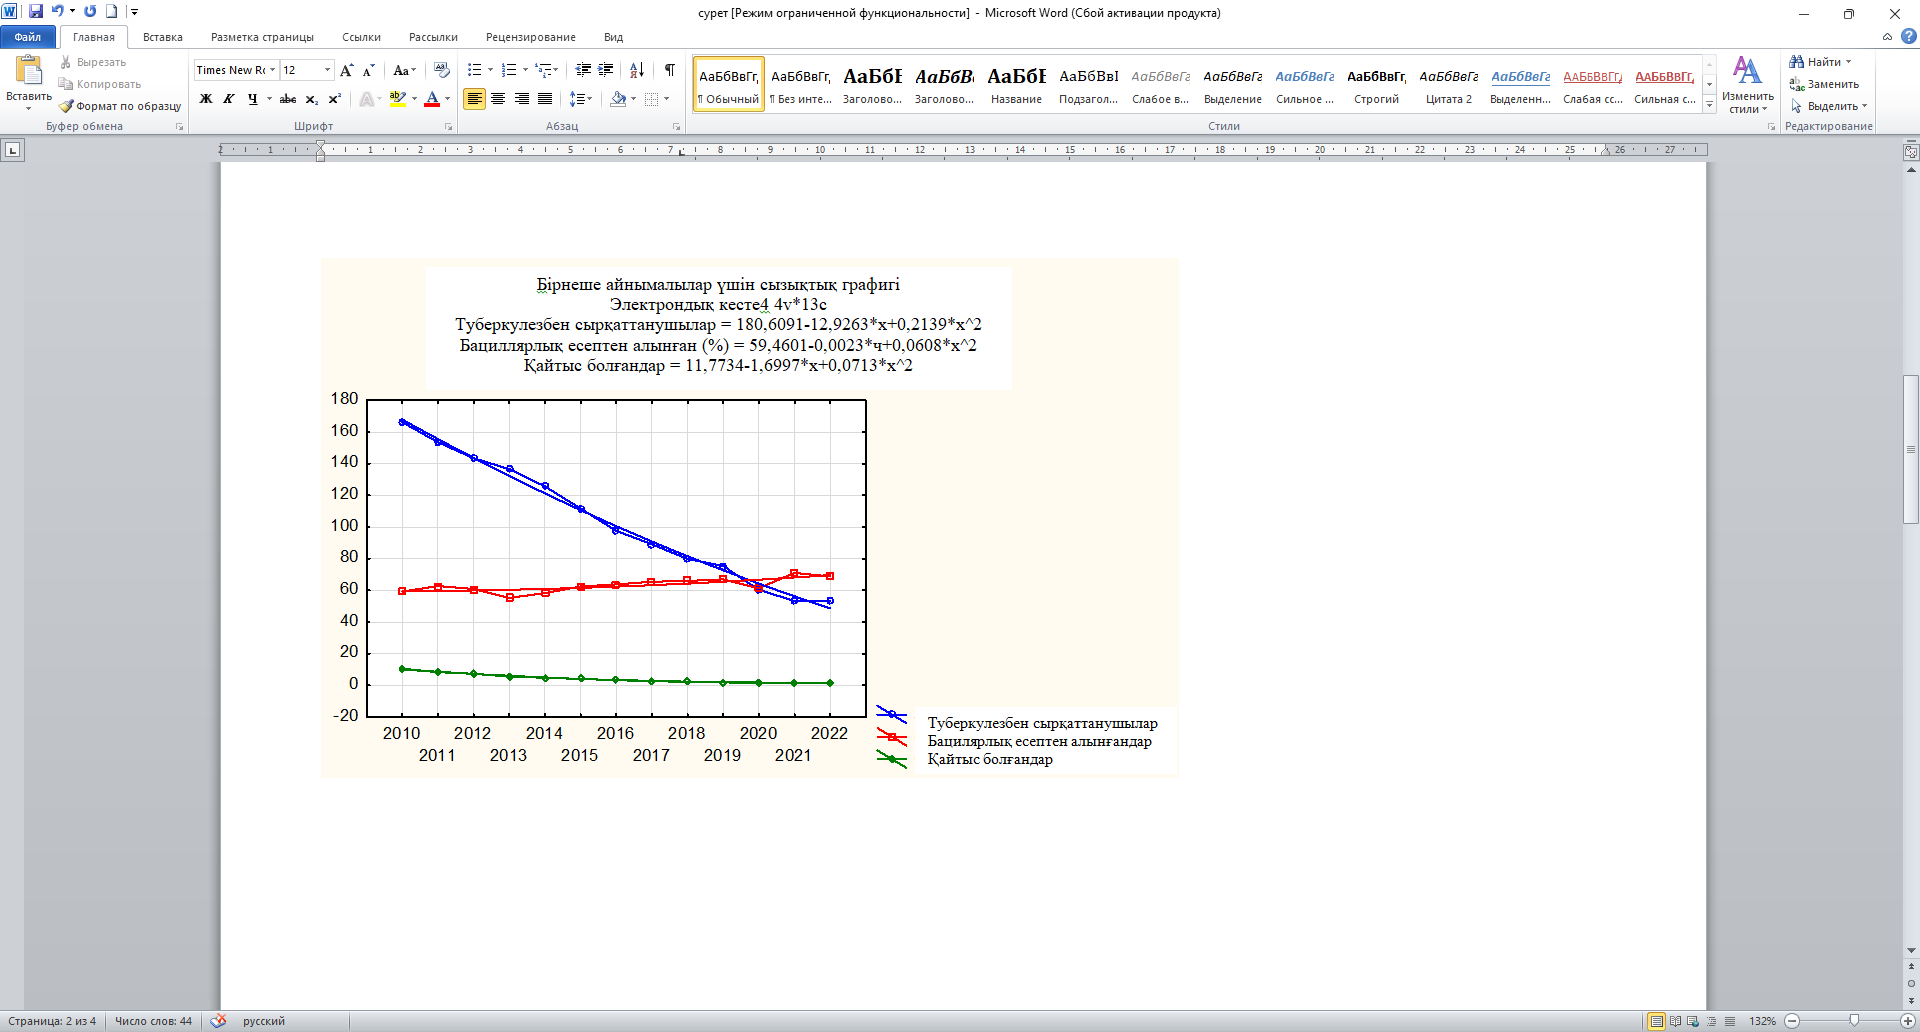
\includegraphics[width=0.8\textwidth]{assets/168}
	\caption*{}
\end{figure}

{\bfseries 1-сурет. Қазақстан Республикасының туберкулезбен
сырқаттанушылығының}

{\bfseries 2010-2022 жылдар аралығындағы динамикасы}

Сызықтық кестеде туберкулезбен ауыратын науқастар (көк сызық) аурушаңдық
2010 жылдан бері тұрақты түрде төмендеп келетіні байқалады. Бұған келесі
факторлар ықпал еткенін көруге болады:

\begin{enumerate}
\def\labelenumi{\arabic{enumi})}
\item
  соңғы жылдары елімізде туберкулезді ерте диагностикалау мен емдеу
  бағдарламаларын қолданып едәуір жақсарғаны. Химиотерапияның қысқа
  курстары сияқты жаңа емдеу әдістерін қолдану аурудың төмендеуіне әсер
  еткен болуы .
\item
  алдын алу шараларын күшейту, соның ішінде БЦЖ (Bacillus
  Calmette-Guérin) жаппай вакцинациялау және санитарлық-ағарту
  жұмыстарын жүргізу де аурудың төмендеуіне ықпал еткен болуы.
\item
  туберкулезбен күресуге бағытталған халықаралық көмек бағдарламалары
  ауруды төмендетуде маңызды рөл атқарғаны байқалады.
\end{enumerate}

Аурудың сызықтық кестесі (1 сурет) туберкулез (науқастардың, қайтыс
болғандардың саны және науқастарды бациллярлық есептен шығару) Қазақстан
Республикасының халқы бойынша 12 жылдық кезеңнің жиынтық деректері
ескеріле отырып 2010-2022 жылдар аралығында қарастырылды. Абсцисса осі
бойынша туберкулезбен ауыратын науқастарды зерттеу жылдары кейінге
қалдырылды, координаттар осі бойынша абсолютті сандар (халықтың 100 000
адамға шаққанда).

Бұл диаграмма 2010 - 2013 жылдар аралығында аурушаңдық бойынша тұрақты
үрдісті көрсетті. Нәтижесінде 2014 жылдан бастап аурушаңдықтың өсуі екі
есе нашарлағаның көріп тұрмыз.

Жалпы республика бойынша сырқаттанушылықтың төмендеуі байқалғанымен,
туберкулез жаңа қасиеттерге ие болды. Науқастарда туберкулез
қоздырғышының дәріге төзбеушілігі және дәріге төзімділігі тұрақты
байқалады (1-сурет).

Жоғарыда көрсетілген кестелерді қарастырсақ, 2010 жылдан бастап
туберкулезбен сырқаттанушылық көрсеткіштерінің күрт төмендегенін бірден
байқауға болады, бірақ 2012 -- 2015 жылдар, 2016-2021 жылдар аралығында
қалыпты өрлеу мен құлдырау анықталуда. Сырқаттанушылық жағдайларының,
бұл күрт төмендеуі елдің туберкулезді инфекциялық бақылау шаралары,
емдеу, диагностика сапасы бойынша жаңа бағыттарға көшуімен байланысты
және туберкулездің алдын алу болып табылады.

Туберкулезді алдын алу, мәселесін шешу үшін эпидемияның болжамды ықтимал
ошағы үлкен рөл атқарады. Сондықтан болжау жүйесін құру немесе
математикалық модельдерді қолдану негіздері бұрыннан қолданғанмен
интеллектуалды жүйелерді пайдалану маңызды болып келеді. Белгілі бір
аймақты нақты және дәл сипаттайтын модельді таңдау жасау.{[}13{]}

{\bfseries Кесте 1.Сипаттамалық статистика нәтижелері}

\begin{longtable}[]{@{}
  >{\raggedright\arraybackslash}p{(\columnwidth - 10\tabcolsep) * \real{0.2315}}
  >{\raggedright\arraybackslash}p{(\columnwidth - 10\tabcolsep) * \real{0.1596}}
  >{\raggedright\arraybackslash}p{(\columnwidth - 10\tabcolsep) * \real{0.1449}}
  >{\raggedright\arraybackslash}p{(\columnwidth - 10\tabcolsep) * \real{0.1450}}
  >{\raggedright\arraybackslash}p{(\columnwidth - 10\tabcolsep) * \real{0.1595}}
  >{\raggedright\arraybackslash}p{(\columnwidth - 10\tabcolsep) * \real{0.1595}}@{}}
\toprule\noalign{}
\multirow{2}{=}{\begin{minipage}[b]{\linewidth}\raggedright
{\bfseries Айнымалы}
\end{minipage}} &
\multicolumn{5}{>{\raggedright\arraybackslash}p{(\columnwidth - 10\tabcolsep) * \real{0.7685} + 8\tabcolsep}@{}}{%
\begin{minipage}[b]{\linewidth}\raggedright
{\bfseries Сипаттамалық статистика}
\end{minipage}} \\
& \begin{minipage}[b]{\linewidth}\raggedright
{\bfseries жарамды N}
\end{minipage} & \begin{minipage}[b]{\linewidth}\raggedright
{\bfseries Орташа}
\end{minipage} & \begin{minipage}[b]{\linewidth}\raggedright
{\bfseries Минимум}
\end{minipage} & \begin{minipage}[b]{\linewidth}\raggedright
{\bfseries Максимум}
\end{minipage} & \begin{minipage}[b]{\linewidth}\raggedright
{\bfseries Стандартты анықтама}
\end{minipage} \\
\midrule\noalign{}
\endhead
\bottomrule\noalign{}
\endlastfoot
Туберкулезбен сырқаттанушы & 13 & 103,6000 & 53,30000 & 166,3000 &
38,90180 \\
Бациллярлық есептен алынды (\%) & 13 & 63,2769 & 55,30000 & 71,1000 &
4,40854 \\
Қайтыс болған & 13 & 4,3692 & 1,40000 & 10,6000 & 2,89349 \\
\end{longtable}

2010-2022 жылдар аралығының кезеңінде туберкулезбен сырқаттанушылықтың
сипаттамалық статистикасын талдау негізінде мынадай тұжырымдар жасауға
болады:(2-сурет)

\begin{itemize}
\item
  туберкулез ауруының орташа жиілігі 103,6000 жағдайды құрайды (халықтың
  100 000 адамға шаққанда)
\item
  ең төменгі мәні туберкулезбен сырқаттанушылық 53,30000(халықтың 100
  000 адамға шаққанда), туберкулезбен сырқаттанушылықтың ең жоғары
  деңгейі 166,30 000(халықтың 100 000 адамға шаққанда) құрайды - бұл
  зерттеу кезеңінде туберкулезбен сырқаттанушылықтың айтарлықтай
  өзгергенің көрсетеді;
\item
  аурудың стандартты ауытқуы 38,90180 бұл орташа мәнге қатысты мәндердің
  таралуын көрсетеді. Стандартты ауытқудың үлкен мәні деректердің
  айтарлықтай өзгергіштігін көрсетеді;
\item
  бациллярлық есептен шығару (яғни туберкулезден айыққан немесе қайтыс
  болған науқастардың саны) орташа мәні 63,2769, ең төменгі мәні 5,30000
  және ең жоғары мәні 71,1000 құрайды. Бұл пациенттердің көпшілігі
  туберкулезден сәтті емделетінін көрсетеді, бірақ өлім жағдайы да бар;
\item
  Туберкулезден болатын өлім-жітімнің орташа мәні 4,3692, ең төменгі
  мәні 1,40000 және ең жоғары мәні 10,6000 -- бұл туберкулезден болатын
  өлім-жітімнің бар екендігін көрсетеді.
\end{itemize}

Негізінде сипаттамалық статистиканың нәтижелері туберкулезбен
сырқаттанушылықтың өзгергіштік деңгейі жоғары екенін көрсетеді,
сондай-ақ осы аурудан сырқаттанушылық пен өлім-жітімді төмендету
шараларын қабылдау қажеттігін көрсетеді.

Деректерді өңдеуге, визуалиациялауға және иерархиялық кластерлеуді
орындау үшін жиі қолданылатын бағдарламалардын бірі Statistica болып
келеді. Осы бағдарлама арқылы деректерді ұқсастығына немесе
айырмашылығына қарай топтастыру үшін Уорд әдісі (Ward's method) және
Манхэттен қашықтығы (City-block, Manhattan distances) сияқты әртүрлі
кластерлеу әдістерін қолданылды. Статистикадағы Дендрограмма
зерттеушілерге күрделі уақыт қатарларын визуализациялауға және талдауға
және анықталған деректер негізінде ақпараттандырылған шешімдер
қабылдауға мүмкіндік береді.

\begin{figure}[H]
	\centering
	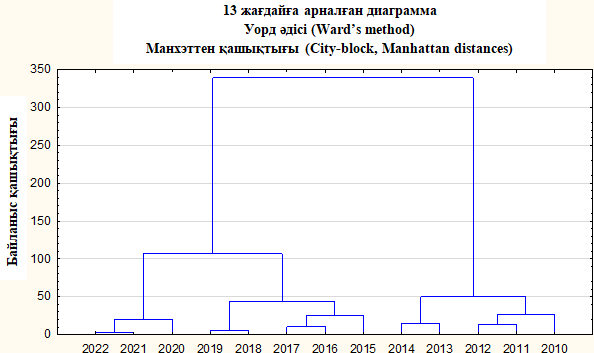
\includegraphics[width=0.8\textwidth]{assets/169}
	\caption*{}
\end{figure}

{\bfseries 2-сурет. Қазақстан Республикасының 2010-2022 жылдар кезеңінде
туберкулезбен сырқаттанушылық жөніндегі Дендрограмма}

Дендрограммада (Сурет 2) көлденең осьта 2010 және 2022 жылдар
аралығындаағы кезеңінде туберкулезбен сырқаттанғаны көрсетілген, ал
тігінен -- бірігу қашықтығын білдіреді. Бүкіл кезең екі үлкен кластерге
бөлінеді: 2010-2014 жылдар және 2015-2022 жылдар. Бұл екі кезеңдегі
туберкулезбен сырқаттанушылық туралы мәліметтер бір-бірінен айтарлықтай
ерекшеленетінін көрсетіп тұр.

1 кластерде 2021-2022, 2019-2020, және 2015-2018 кіші топтарға бөлінген

Соңғы 2021 және 2022 жылдар жеке кіші топты құрайды, бұл осы кезеңдегі
аурудың ерекше динамикасын көрсетіп тұрғанын көреміз, мүмкін соңғы
жылдары қабылданған шаралармен немесе есептіліктің өзгеруімен
байланысты. 2019 және 2020 жылдар да бөлек топтастырылған, бұл COVID-19
пандемиясының осы кезеңдегі туберкулез статистикасына әсерін көрсетуі
деп білеміз

2 кластер 2010-2014 жылдар аралығы көрсеткіштері тұрақтылықты көрсетіп
тұр.

Дендрограмма туберкулезбен ауыру динамикасында, әсіресе 2014-2015 жылдар
аралығында айтарлықтай өзгерістердің болуын болжайды, бұл емдеу
стратегияларының, Денсаулық сақтау саясатының немесе басқа сыртқы
факторлардың өзгеруіне байланысты болуы мүмкін.Соңғы жылдардағы кіші
топтар (2019-2022) талдау үшін ерекше назар аударуды қажет етеді,
өйткені олар ауру динамикасындағы жаңа бағытты көрсете алады.

Бұл деректер белгілі бір кезеңде туберкулез ауруының мұндай өзгеруіне не
себеп болуы мүмкін екенін жақсы түсіну үшін қосымша талдау үшін қажет
етеді.

Statistica бағдарламасында жасалған дендрограмма нақты математикалық
модельдерге негізделген иерархиялық деректер кластерінің визуализациясы
болып табылады. Бұл дендрограмма кластерлерді біріктіру үшін Уорд әдісін
және деректер арасындағы қашықтықты есептеу үшін Манхэттен қашықтығын
(City-block, Manhattan distances) пайдаланады.{[}14{]}

Оларды бөлек талдап көретін болсақ:

Уорд әдісінің (Ward's method) (формула2) мақсаты кластерлерді
біріктірудің әрбір қадамында жалпы кластерішілік дисперсияның ұлғаюын
азайту.

\begin{figure}[H]
	\centering
	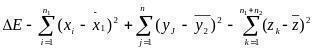
\includegraphics[width=0.8\textwidth]{assets/170}
	\caption*{}
\end{figure} (1)

Бұндағы:

\begin{figure}[H]
	\centering
	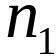
\includegraphics[width=0.8\textwidth]{assets/171}
	\caption*{}
\end{figure} және
\begin{figure}[H]
	\centering
	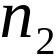
\includegraphics[width=0.8\textwidth]{assets/172}
	\caption*{}
\end{figure}- 1 және 2 кластерлердегі элементтер
саны.

\begin{figure}[H]
	\centering
	
\includegraphics[width=0.8\textwidth]{assets/173}
	\caption*{}
\end{figure} және
\begin{figure}[H]
	\centering
	
\includegraphics[width=0.8\textwidth]{assets/174}
	\caption*{}
\end{figure}- 1 және 2 кластер элементтері

\begin{figure}[H]
	\centering
	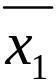
\includegraphics[width=0.8\textwidth]{assets/175}
	\caption*{}
\end{figure} және
\begin{figure}[H]
	\centering
	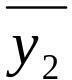
\includegraphics[width=0.8\textwidth]{assets/176}
	\caption*{}
\end{figure} - 1 және 2 кластерлер бойынша орташа
мәндер.

\begin{figure}[H]
	\centering
	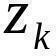
\includegraphics[width=0.8\textwidth]{assets/177}
	\caption*{}
\end{figure} - біріктірілген кластер элементтері.

\begin{figure}[H]
	\centering
	
\includegraphics[width=0.8\textwidth]{assets/178}
	\caption*{}
\end{figure} - біріктірілген кластердің орташа
мәні.

Уорд әдісінің (Ward's method) мақсаты
\begin{figure}[H]
	\centering
	
\includegraphics[width=0.8\textwidth]{assets/179}
	\caption*{}
\end{figure} азайту болып келеді бұл екі
кластерді біріктіру кезінде кластер ішіндегі дисперсияның өзгеруін
білдіреді..

Манхэттен қашықтығы (City-block, Manhattan distances) (формула 2)әдістің
мақсаты: жылдар арасындағы ұқсастықтарды есептеу үшін қолданылатын көп
өлшемді кеңістіктегі екі нүкте арасындағы қашықтықты анықтау болып
табылады.

\begin{figure}[H]
	\centering
	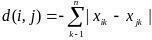
\includegraphics[width=0.8\textwidth]{assets/180}
	\caption*{}
\end{figure} (2)

Бұндағы:

\begin{figure}[H]
	\centering
	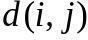
\includegraphics[width=0.8\textwidth]{assets/181}
	\caption*{}
\end{figure} - Манхэттеннің нүктелер арасындағы
қашықтығы
\begin{figure}[H]
	\centering
	
\includegraphics[width=0.8\textwidth]{assets/182}
	\caption*{}
\end{figure}\begin{figure}[H]
	\centering
	
\includegraphics[width=0.8\textwidth]{assets/182}
	\caption*{}
\end{figure}\begin{figure}[H]
	\centering
	
\includegraphics[width=0.8\textwidth]{assets/183}
	\caption*{}
\end{figure}
және \begin{figure}[H]
	\centering
	
\includegraphics[width=0.8\textwidth]{assets/184}
	\caption*{}
\end{figure}

\begin{figure}[H]
	\centering
	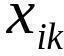
\includegraphics[width=0.8\textwidth]{assets/185}
	\caption*{}
\end{figure} және
\begin{figure}[H]
	\centering
	
\includegraphics[width=0.8\textwidth]{assets/186}
	\caption*{}
\end{figure} -\begin{figure}[H]
	\centering
	
\includegraphics[width=0.8\textwidth]{assets/182}
	\caption*{}
\end{figure}
\begin{figure}[H]
	\centering
	
\includegraphics[width=0.8\textwidth]{assets/187}
	\caption*{}
\end{figure} және
\begin{figure}[H]
	\centering
	
\includegraphics[width=0.8\textwidth]{assets/188}
	\caption*{}
\end{figure} нүкте координаттарының
\begin{figure}[H]
	\centering
	
\includegraphics[width=0.8\textwidth]{assets/189}
	\caption*{}
\end{figure} өлшемі

\begin{figure}[H]
	\centering
	
\includegraphics[width=0.8\textwidth]{assets/190}
	\caption*{}
\end{figure} - өлшеу саны

Манхэттен қашықтығы (City-block, Manhattan distances)әр өлшемдегі
нүктелердің координаттары арасындағы жалпы абсолютті айырмашылықты
өлшейді.

Дендрограмманың жалпы моделі:

\begin{enumerate}
\def\labelenumi{\arabic{enumi}.}
\item
  Кластерлеудің әр кезеңінде екі кластер таңдалады, олардың арасындағы
  қашықтық Манхэттен метрикасы бойынша минималды. Содан кейін бұл
  кластерлер біріктіріліп, процедура барлық нысандар бір кластерде
  болғанша қайталанады.
\item
  Біріктіру процесі Уорд әдісін (Ward's method) қолдану арқылы қол
  жеткізілетін кластерішілік дисперсияның ұлғаюын азайту үшін жүреді.
\end{enumerate}

Осылайша, дендрограмма кластер ішіндегі дисперсияны азайту және
Манхэттен метрикасы бойынша қашықтықты есептеу негізінде кластерлерді
дәйекті біріктіру процесінің графикалық көрінісі болып табылады.

{\bfseries Нәтижелер мен талқылау.} Бұл зерттеу туберкулез сияқты ауруларды
бақылау және талдау саласына маңызды үлес қосады. Деректер мен
математикалық модельдерді қолдану аурудың динамикасын түсінуге ғана
емес, сонымен қатар аурудың таралуына әсер ететін факторларды анықтауға
мүмкіндік береді. Деректерді жинауды, өңдеуді және талдауды
автоматтандыруға қабілетті интеграцияланған ақпараттық жүйелерді дамыту
ауруларды тиімді бақылау мен бақылаудың негізгі элементі болып табылады.
Зерттеу қоғамдық денсаулық пен халықтың өмір сүру сапасын жақсарту үшін
деректерді өндіру саласындағы жұмыстарды жалғастырудың маңыздылығын
көрсетеді.

Туберкулез сияқты әлеуметтік маңызы бар аурулардың мониторингінде
деректерді интеллектуалды талдауды қолдану оның болашақ даму үшін
маңыздылығы мен әлеуетін көрсетеді. Data Mining математикалық модельдері
мен әдістеріне негізделген зерттеу 2010-2022 жылдар аралығында Қазақстан
Республикасында туберкулезбен сырқаттанушылықтың динамикасын терең
түсіну мүмкіндіктерін көрсетеді, бұл мақсатты профилактикалық және емдік
іс-шараларды әзірлеуге ықпал ететін үрдістер мен ықпал ететін
факторларды анықтайды. Деректерді интеллектуалды талдау
сырқаттанушылықтың динамикасын көзбен көріп, болжап қана қоймай, сонымен
қатар халықтың көші-қоны, өмір сүру деңгейі, медициналық қызмет көрсету
деңгейі, медициналық қызмет көрсету шығындары сияқты сырқаттанушылық пен
басқа да әлеуметтік маңызы бар факторлар арасында байланыс орнатуға,
түрлі аймақтар бойынша талдау жүргізуге мүмкіндік береді.

Демек, ауру деректерін автоматтандырылған бақылау мен талдауға арналған
интеграцияланған ақпараттық жүйені әзірлеу және енгізу қажеттілігі
туындайды.

Мұндай жүйе талдау және болжау құралдарын ұсына отырып, деректерді
жинауды, өңдеуді және сақтауды жақсартуға уәде береді, бұл ауру деңгейін
тиімдірек төмендетуге және эпидемиологиялық қауіптерге жауап беруге
мүмкіндік береді.{[}15{]}

Алдын ала талдау жоспарланған ақпараттық жүйе мынадай блоктардан тұруы
тиіс екенін көрсетті: деректерді қабылдау, тазарту, трансформациялау;
деректер қоймасы; деректерді статистикалық талдау блогы; деректерді
интеллектуалды талдау блогы; болжамдарды қалыптастыру блогы; есептерді
қалыптастыру блогы; деректерді визуализациялау блогы.

Зерттеудің маңыздылығы: деректерді жинау, өңдеу және талдау процестерін
автоматтандырудың қоғамдық денсаулық сақтауды жақсартудағы маңыздылығын
айқын көрсетеді. Интеграцияланған ақпараттық жүйелердің көмегімен үлкен
көлемдегі деректерді тиімді басқару және талдау аурудың таралу
динамикасын жақсы түсінуге мүмкіндік береді. Мұндай жүйелер нақты
уақыттағы эпидемияларды анықтау және алдын алу үшін аса қажет.

Зерттеу нәтижесінде 2010-2022 жылдар аралығында туберкулездің таралуы
бойынша деректерге негізделген болжау жасалды. Data Mining және
статистикалық әдістері туберкулезбен сырқаттанушылықтың болашақ
динамикасын анықтауға және соған сәйкес алдын алу шараларын жоспарлауға
мүмкіндік береді. Мысалы, 2020-2022 жылдардағы дендрограмма мен
графиктерде көрінген ауру деңгейінің өзгерістері емдеу және алдын алу
шараларының тиімділігін көрсетті.

Алынған нәтижелер 2010-2022 жылдардағы туберкулезбен сырқаттанушылық пен
өлім-жітім динамикасында айтарлықтай төмендеу байқалғанын көрсетеді.
Сырқаттанушылықтың төмендеуі денсаулық сақтау жүйесінде жүргізілген
алдын алу және емдеу шараларының тиімділігін көрсетсе, өлім-жітімнің
төмендеуі тиімді емдеу шараларының нәтижесі болуы мүмкін.

Деректерді интеллектуалды өңдеу арқылы аурудың таралуына әсер ететін
негізгі факторлар анықталды. Бұл факторлар туберкулездің аймақтық
ерекшеліктеріне, халықтың әлеуметтік-экономикалық жағдайына және
медициналық ресурстардың қолжетімділігіне байланысты болуы
мүмкін.Туберкулездің таралуын болжау және негізгі факторларды анықтау
болашақта мақсатты профилактикалық іс-шараларды ұйымдастыруға ықпал
етеді. Бұл алынған мәліметтерді емдеу стратегияларын жетілдіру үшін
қолдануға болады.

Зерттеу барысында жасалған математикалық модельдер мен статистикалық
әдістер Қазақстан Республикасында туберкулездің өршігу динамикасын
тереңірек түсінуге мүмкіндік берді. Деректерді интеллектуалды өңдеу
нәтижесінде алынған нәтижелер туберкулездің өршігуне әсер ететін негізгі
факторларды анықтап қана қоймай, оның болашақта қалай жетілуінің
болжауға көмектеседі. Бұл ауруды бақылау және алдын алу шараларын
жетілдіру үшін маңызды ақпарат болып табылады. Туберкулездің таралуын
болжау бойынша алынған нәтижелер денсаулық сақтау жүйесіне орасан зор
үлес қосып, оның қоғамдық денсаулыққа әсерін азайтуға мүмкіндік береді.

{\bfseries Қорытынды.} Бұл зерттеу Қазақстан Республикасында 2010-2022
жылдар аралығындағы туберкулезбен сырқаттанушылықтың динамикасын талдау
арқылы әлеуметтік маңызы бар ауруларды бақылаудың заманауи әдістерінің
маңыздылығын көрсетіп, деректерді интеллектуалды өңдеу мен математикалық
модельдеу әдістерін қолдану барысында туберкулез аурудын таралуын, оның
өлім-жітім көрсеткіштерін және емдеу нәтижелерін болжауға мүмкіндік
берді.

Зерттеу барысында туберкулездің өршігу динамикасын талдау үшін деректер
арасындағы айырмашылықтарды анықтау үшін, Манхэттен
қашықтығы(City-block, Manhattan distances) және Уорд
(Ward\textquotesingle s Method) кластерлеу әдістері қолданылып
объектілер арасындағы айырмашылықтарды бірқатар факторлар бойынша
өлшеуге мүмкіндік берді. Нәтижесінде, туберкулезбен сырқаттанушылықтың
әртүрлі жылдардағы деңгейлерінің ұқсастығы мен айырмашылықтары
анықталды.

Ал, Уорд әдісі (Ward\textquotesingle s Method) кластерлеуді жүргізу
барысында топтар арасындағы дисперсияны минимизациялау принципіне
негізделіп, деректерді ұқсас топтарға біріктіру арқылы жылдар арасындағы
корреляцияны айқындап, туберкулездің өршігу үрдістерін көрсететін
иерархиялық құрылымдарды жасауға мүмкіндік берді.

Нәтижесінде, белгілі бір жылдар арасындағы сырқаттанушылықтың өзара
ұқсастықтары анықталып, дендрограммада құрылды.

Уорд әдісі (Ward\textquotesingle s Method) мен Манхэттен қашықтығын
(City-block, Manhattan distances) қолдану эпидемиологиялық деректерді
топтастыруда және оларды талдауда тиімді әдіс ретінде маңызды рөл
атқаратыны, туберкулез ауруының өршігуі бойынша динамикалық өзгерістерді
айқындауға, әртүрлі жылдардағы сырқаттанушылардың көрсеткіштерінің ұқсас
кезеңдерін анықтауға және оларды болашақта болжау үшін қолдануға
болатыны дәлелденді деуге болады.

Алынған нәтижелер денсаулық сақтау жүйесіне стратегиялық шешімдер
қабылдауда нақты негізі болып, эпидемиологиялық жағдайды тиімді
басқаруға ықпал етеді.

Бұл әдістер эпидемияларды уақтылы анықтау, тиімді бақылау және олардың
әсерін азайту үшін денсаулық сақтау жүйесін оңтайландыруға көмектеседі.

Қорытындылай келе, туберкулездің таралуын болжау мақсатында заманауи
әдістерді қолдану Қазақстандағы қоғамдық денсаулықты жақсарту және осы
аурумен күрестің тиімділігін арттыру үшін маңызды қадам болып табылады.

{\bfseries Әдебиеттер}

\begin{enumerate}
\def\labelenumi{\arabic{enumi}.}
\item
  Кубегенова А., Искаков К., Кубегенов Е., Криворотько О. Мониторинг и
  моделирование эпидемиологической ситуации с помощью интеллектуального
  анализа данных // Известия НАН РК. Серия физико-математическая. -№
  4(2022). --С. 43-55. DOI: https://doi.org/10.32014/2022.2518-1726.155
\item
  Юнкеров В.И. Математико-статистическая обработка данных медицинских
  исследований / В.И. Юнкеров, С.Г. Григорьев. -- СПб.: ВМедА, 2002. --
  266 с. ISBN 5-94277-011-5
\item
  Барсегян А. А. С. Куприянов, И. И. Холод, М. Д. Тесс, С.И. Елизаров
  Анализ данных и процессов: учеб. пособие /-- 3-е изд., перераб. и доп.
  -- СПб.: БХВ-Петербург, 2009-- 512 с. ISBN 978-5-9775-0368-6
\item
  Xinyi Wang. The Role of Data Mining Technology in Advertising
  Marketing // J. Phys.: Conf. Ser. -2021. --Vol. 1744(4). DOI:
  10.1088/1742-6596/1744/4/042202
\item
  Jianguo Liu \& Sheng Zhou~Application Research of Data Mining
  Technology in Personal Privacy Protection and Material Data Analysis
  // Integrated Ferroelectrics. -2021. --Vol.216. --P. ~29-42.
  DOI:~10.1080/10584587.2021.1911255
\item
  He, Wu, Gongjun Yan, and Li Da Xu. Developing vehicular data cloud
  services in the IoT environment // IEEE
  transactionsonindustrialinformatics. -2014. --Vol. 10(2). -P.
  1587-1595. DOI:10.1109/TII.2014.2299233
\item
  Peña-Ayala, Alejandro Educational data mining: A survey and a data
  mining-based analysis of recent works // Expertsystemswith
  applications. -2014. --Vol.41(4). --Vol.1432-1462.
  DOI:10.1016/j.eswa.2013.08.042
\item
  Zhenhua HUANG, Zhenyu WANG,~Li JIANG,~Rui ZHANG,~Chang LEI,~Xingwei
  LIU,~Xiaohui XIE Analysis of COVID-19 spread characteristics and
  infection numbers based on large-scale structured case data //
  Scientia Sinica Informationis. -2020--Vol. 50(12).
  DOI:10.1360/SSI-2020-0029
\item
  Cross C. L. Statistical and methodological considerations when using
  cluster analysis in neuropsychological research //Cluster analysis in
  neuropsychological research: Recent applications. -- New York, NY :
  Springer New York, 2013. --Vol. 25(5). -- P. 13-35.
  DOI:10.1007/978-1-4614-6744-1\_2
\item
  Мельниченко О.А., Романюха А.А. Модель эпидемиологии туберкулеза.
  Анализ данных и оценка параметров // Математическое моделирование. --
  2008. -- №8. -- С.107-128. URL:
  https://www.mathnet.ru/links/8eaf4b16128064394600eb860acd44ba/mm2678.pdf
\item
  Генеральная Ассамблея. Организация Объединенных Наций.
  https://documents.un.org/doc/undoc/gen/n23/306/93/pdf/n2330693.pdf
\item
  Национальный научный центр развития здравоохранения имени
  С.Каирбекова. Статистические сборники «Здоровье населения~ Республики
  Казахстан и деятельность организаций~ здравоохранения».~
\end{enumerate}

URL:
https://nrchd.kz/index.php/ru/?option=com\_content\&view=article\&id=973

\begin{enumerate}
\def\labelenumi{\arabic{enumi}.}
\setcounter{enumi}{12}
\item
  Kubegenova, A.D., Zhakhiena, A.G., Baigubenova, S.K., Utyasheva, G.S.,
  Omarov, A.N. Clustering and data mining on the example of hiv-infected
  people data\\
  \emph{//~}Journal of Theoretical and Applied Information
  Technology\emph{.} -2022. --Vol.100~(13). -P.~5010-5018. URL:
  https://jatit.org/volumes/Vol100No13/30Vol100No13.pdf
\item
  King R. S. Cluster analysis and data mining: An introduction. --
  Mercury Learning and Information, 2015. ISBN 978-1-938549-38-0
\item
  Kubegenova A.D.,KamalovaG.A., Kubegenov, E.S., Gumarova, Z.M.,
  Zhazykbaeva, G.M. Using Data Mining Technology in Monitoring and
  Modeling the Epidemiological Situation of the Human Immunodeficiency
  Virus in Kazakhstan // Information Technologies and Intelligent
  Decision-Making Systems. -2022. -Vol 1703. --P. 57-65.
  DOI:10.1007/978-3-031-21340-3\_6
\end{enumerate}

{\bfseries References}

1. Kubegenova A., Iskakov K., Kubegenov E., Krivorot\textquotesingle ko
O. Monitoring i modelirovanie jepidemiologicheskoj situacii s
pomoshh\textquotesingle ju intellektual\textquotesingle nogo analiza
dannyh // Izvestija NAN RK. Serija fiziko-matematicheskaja. -№ 4(2022).
--S. 43-55. DOI: https://doi.org/10.32014/2022.2518-1726.155 {[}in
Russian{]}

2. Junkerov V.I. Matematiko-statisticheskaja obrabotka dannyh
medicinskih issledovanij / V.I. Junkerov, S.G.
Grigor\textquotesingle ev. -- SPb.: VMedA, 2002. -- 266 s. ISBN
5-94277-011-5 {[}in Russian{]}

3. Barsegjan A. A. S. Kuprijanov, I. I. Holod, M. D. Tess, S.I. Elizarov
Analiz dannyh i processov: ucheb. posobie /-- 3-e izd., pererab. i dop.
-- SPb.: BHV-Peterburg, 2009-- 512 s. ISBN 978-5-9775-0368-6 {[}in
Russian{]}

4. Xinyi Wang. The Role of Data Mining Technology in Advertising
Marketing // J. Phys.: Conf. Ser. -2021. --Vol. 1744(4). DOI:
10.1088/1742-6596/1744/4/042202

5. Jianguo Liu \& Sheng Zhou Application Research of Data Mining
Technology in Personal Privacy Protection and Material Data Analysis //
Integrated Ferroelectrics. -2021. --Vol.216. --P. 29-42. DOI:
10.1080/10584587.2021.1911255

6. He, Wu, Gongjun Yan, and Li Da Xu. Developing vehicular data cloud
services in the IoT environment // IEEE
transactionsonindustrialinformatics. -2014. --Vol. 10(2). -P. 1587-1595.
DOI:10.1109/TII.2014.2299233

7. Peña-Ayala, Alejandro Educational data mining: A survey and a data
mining-based analysis of recent works // Expertsystemswith applications.
-2014. --Vol.41(4). --Vol.1432-1462. DOI:10.1016/j.eswa.2013.08.042

8. Zhenhua HUANG, Zhenyu WANG, Li JIANG, Rui ZHANG, Chang LEI, Xingwei
LIU, Xiaohui XIE Analysis of COVID-19 spread characteristics and
infection numbers based on large-scale structured case data // Scientia
Sinica Informationis. -2020--Vol. 50(12). DOI:10.1360/SSI-2020-0029

9. Cross C. L. Statistical and methodological considerations when using
cluster analysis in neuropsychological research //Cluster analysis in
neuropsychological research: Recent applications. -- New York, NY :
Springer New York, 2013. --Vol. 25(5). -- P. 13-35.
DOI:10.1007/978-1-4614-6744-1\_2

10. Mel\textquotesingle nichenko O.A., Romanjuha A.A.
Model\textquotesingle{} jepidemiologii tuberkuleza. Analiz dannyh i
ocenka parametrov // Matematicheskoe modelirovanie. -- 2008. -- №8. --
S.107-128. URL:
https://www.mathnet.ru/links/8eaf4b16128064394600eb860acd44ba/mm2678.pdf
{[}in Russian{]}

11. General\textquotesingle naja Assambleja. Organizacija Ob\#edinennyh
Nacij.
https://documents.un.org/doc/undoc/gen/n23/306/93/pdf/n2330693.pdf {[}in
Russian{]}

12. Nacional\textquotesingle nyj nauchnyj centr razvitija
zdravoohranenija imeni S.Kairbekova. Statisticheskie sborniki
«Zdorov\textquotesingle e naselenija Respubliki Kazahstan i
dejatel\textquotesingle nost\textquotesingle{} organizacij
zdravoohranenija».

URL:
https://nrchd.kz/index.php/ru/?option=com\_content\&view=article\&id=973
{[}in Russian{]}

13. Kubegenova, A.D., Zhakhiena, A.G., Baigubenova, S.K., Utyasheva,
G.S., Omarov, A.N. Clustering and data mining on the example of
hiv-infected people data

// Journal of Theoretical and Applied Information Technology. -2022.
--Vol.100 (13). -P. 5010-5018. URL:
https://jatit.org/volumes/Vol100No13/30Vol100No13.pdf

14. King R. S. Cluster analysis and data mining: An introduction. --
Mercury Learning and Information, 2015. ISBN 978-1-938549-38-0

15. Kubegenova A.D.,KamalovaG.A., Kubegenov, E.S., Gumarova, Z.M.,
Zhazykbaeva, G.M. Using Data Mining Technology in Monitoring and
Modeling the Epidemiological Situation of the Human Immunodeficiency
Virus in Kazakhstan // Information Technologies and Intelligent
Decision-Making Systems. -2022. -Vol 1703. --P. 57-65.
DOI:10.1007/978-3-031-21340-3\_6

\emph{{\bfseries Information about the authors}}

Kubegenov E.S. -- Senior Lecturer, Zhangir Khan West Kazakhstan Agrarian
Technical University, Uralsk, Kazakhstan, e-mail: erlando78@mail.ru;

Kubegenova A.D. -- Senior Lecturer, Master\textquotesingle s degree,
Zhangir Khan West Kazakhstan Agrarian Technical University, Uralsk,
Kazakhstan, e-mail: aigul-03@mail.ru;

Zhakhiena A.G. - Senior Lecturer, Master\textquotesingle s degree,
Zhangir Khan West Kazakhstan Agrarian Technical University, Uralsk,
Kazakhstan, e-mail: aizatmail@mail.ru;

Utesheva G.Sh.- Senior Lecturer, Master\textquotesingle s degree, West
Kazakhstan University of Innovation and Technology, Uralsk, Kazakhstan,
e-mail:utesheva.gulnara@mail.ru;

Nesterov A.V.- Ph.D., Professor Plekhanov Russian University of
Economics, Moscow, Russia, e-mail: nesterov.av@rea.ru

\emph{{\bfseries Сведения об авторах}}

Кубегенов Е.С. -- старший преподователь,Западно-Казахстанский
аграрно-технический университет имени Жангир хана, Уральск,
Казахстан,e-mail:erlando78@mail.ru;

Кубегенова А. Д. -- старший преподаватель, магистр Западно-Казахстанский
аграрно-технический университет имени Жангир хана, Уральск,
e-mail:aigul-03@mail.ru;

Жахиена А.Г.- старший преподаватель,магистр, Западно-Казахстанский
аграрно-технический университет имени Жангир хана, Уральск, Казахстан,
e-mail: aizatmail@mail.ru;

Утешева Г.Ш.-старший преподаватель, магистр, Западно-Казахстанский
инновационно-технологический университет, Уральск, Казахстан, e-mail:
utesheva.gulnara@mail.ru;

Нестеров А.В. - д.ф.м.н., профессор, Российский экономический
университет им. Г.В. Плеханова, Москва, Россия, e-mail:
nesterov.av@rea.ru\newpage
{\bfseries ҒТАМР 20.53.19}

{\bfseries МЕДИЦИНА САЛАСЫНДА КОМПЬЮТЕРЛІК КӨРУ ӘДІСТЕРІНІҢ}

{\bfseries НЕГІЗІНДЕ} {\bfseries ГРАФИКАЛЫҚ АҚПАРАТТЫ ӨҢДЕУ}

{\bfseries Ж.С.~Есенгалиева\textsuperscript{🖂}, Ж.О. Оралбекова, М.К.
Турарова}

Л.Н.~Гумилев атындағы Еуразия ұлттық университеті, Астана, Қазақстан,

{\bfseries \textsuperscript{🖂,}}Корреспондент-автор: jannayess@gmail.com

Мақалада медициналық бейнелерді талдауда қолданылатын сегменттеу
әдістері сипатталған. Магниттік резонансты томография және компьютерлік
томография кескіндерін талдауда қолданылатын шекті мәндер,
классификация, кластерлеу, Марков желілері, нейрондық желілер,
деформацияланатын модельдер сияқты әдістердің артықшылықтары мен
кемшіліктері қарастырылады. Денсаулық сақтау саласында компьютерлік
көруді пайдалана отырып, графикалық деректерді өңдеуге арналған
бағдарламалық қамтамасыз ету технологиясын әзірлеу процесі ұсынылған.
Әзірленген жүйені жобалау және модельдеу кезеңдері сипатталған. Кескінді
сегменттеу арқылы деректерді өңдеу диагностикалық дәлдікке және қолданба
пайдаланушылары арасындағы тығыз өзара әрекеттесуге ықпал етеді.
Сондай-ақ, қолданбалар бұлтында зерттеу көлемін сақтауға мүмкіндік
беретін дерекқор және кросс-платформалық қосымша жасалды. Құрылған
мобильді қосымшаны толық тестілеу жүргізілді. Денсаулық сақтау саласында
медициналық кескінді сегменттеу дәлірек диагноз қою және пациенттің
диагнозын одан әрі тексеру үшін барған сайын қажетті функцияға айналуда.
Сондықтан түрлі ауруларды дер кезінде анықтаудың арқасында ол неғұрлым
ұтымды әрі мақсатты емделуде, халықтың өмір сүру сапасын жақсартуда
кеңінен пайдаланылмақ. Қолданбаны әзірлеу кезінде графикалық деректерді
талдауды жеңілдететін Open CV, Tensorflow, PyTorch кітапханаларды
қолдану арқылы деректерді өңдеу жүргізілді.

{\bfseries Түйін сөздер:} компьютерлік көру, OpenCV, Tensorflow,
сегментация, графикалық деректерді өңдеу.

{\bfseries ОБРАБОТКА ГРАФИЧЕСКИХ ДАННЫХ НА ОСНОВЕ МЕТОДОВ}

{\bfseries КОМПЬЮТЕРНОГО ЗРЕНИЯ В СФЕРЕ МЕДИЦИНЫ}

{\bfseries Ж.С.~Есенгалиева\textsuperscript{🖂}, Ж.О. Оралбекова,
М.К.~Турарова}

Евразийский национальный университет имени Л.Н.~Гумилева, Астана,
Казахстан,

e-mail: jannayess@gmail.com

В статье описаны методы сегментации, используемые при анализе
медицинских изображений. Рассмотрены преимущества и недостатки таких
методов как пороговые значения, классификация, кластеризация, Марковские
сети, нейронные сети, деформируемые модели, используемых при анализе
изображений магнитно-резонансной томографии и компьютерной томографии.
Представлен процесс разработки программной технологии обработки
графических данных с использованием компьютерного зрения в сфере
здравоохранения. Описаны этапы проектирования и моделирования
разработанной системы. Обработка данных посредством сегментации
изображений способствует точности диагностирования и тесного
взаимодействия между пользователями приложения. Также создана база
данных и кроссплатформенное приложение, позволяющее хранить объем
исследований в облаке приложений. Проведено полное тестирование
созданного мобильного приложения. В сфере здравоохранения сегментация
медицинских изображений становится все наиболее необходимой функцией для
более точной диагностики и дальнейшей верификации диагноза пациента, а
потому, благодаря своевременному выявлению различных заболеваний, будет
широко использоваться для более рационального и целенаправленного
лечения, улучшающее качество жизни населения. При разработке приложения
обработка данных осуществлялась с помощью таких библиотек, как OpenCV,
Tensorflow, PyTorch, которые способствуют анализу графических данных.

{\bfseries Ключевые слова:} компьютерное зрение, OpenCV, Tensorflow,
сегментация, обработка графических данных.

{\bfseries PROCESSING OF GRAPHIC DATA BASED ON COMPUTER VISION METHODS}

{\bfseries IN THE FIELD OF MEDICINE}

{\bfseries Zh.S. Yessengaliyeva\textsuperscript{🖂}, Zh.O. Oralbekova, M.K.
Turarova}

L.N. Gumilyov Eurasian national university, Astana, Kazakhstan,

e-mail: jannayess@gmail.com

The article describes segmentation methods used in the analysis of
medical images. The advantages and disadvantages of such methods as
threshold values, classification, clustering, Markov networks, neural
networks, deformable models used in the analysis of magnetic resonance
imaging and computed tomography images are considered. The process of
developing software technology for processing graphic data using
computer vision in the healthcare sector is presented. The stages of
design and modeling of the developed system are described. Data
processing through image segmentation promotes diagnostic accuracy and
close interaction between application users. A database and
cross-platform application have also been created that allows you to
store a volume of research in the application cloud. Full testing of the
created mobile application was carried out. In the healthcare sector,
medical image segmentation is becoming an increasingly necessary
function for more accurate diagnosis and further verification of the
patient's diagnosis, and therefore, thanks to the timely detection of
various diseases, it will be widely used for more rational and targeted
treatment, improving the quality of life of the population. When
developing the application, data processing was carried out using
libraries such as OpenCV, Tensorflow, PyTorch, which facilitate the
analysis of graphical data.

{\bfseries Key words:} computer vision, OpenCV, Tensorflow, segmentation,
processing of graphic data.

{\bfseries Кіріспе.} Компьютерлік көру айналасындағы заттарды қабылдауға,
жіктеуге, тануға және жауап беруге мүмкіндік береді. Медициналық
кескінді өңдеу, іздеу мен талдауды жеңілдету үшін өңделмеген кескіндерді
өлшенетін символдық пішінге түрлендіру, диагностикаға көмектесу үшін
мәнді сандық ақпаратты алу және көптеген кескіндеу әдістерінен қосымша
деректерді біріктіру үшін пайдалы. Медициналық кескінді талдаудың іргелі
мәселелерінің бірі кескіндердегі органдар немесе қалыптан тыс аймақтар
(мысалы, ісіктер) сияқты объектілердің шекараларын анықтайтын кескін
сегментациясы болып табылады. Сегменттеу нәтижесінің болуы пішінді
талдауға, көлемнің өзгеруін анықтауға және дәл сәулелік терапия
жоспарына мүмкіндік береді.

Жақында медициналық кескіндерді сегментациялау әдебиетінде бірнеше жалпы
әдістер пайда болды {[}1{]}. Сегменттеу әдістерін келесі санатқа
бөлеміз: шекті мән тәсілдері, аймақты кеңейту тәсілдері, жіктеуіштер,
кластерлеу тәсілдері, Марковтың кездейсоқ өріс модельдері (MRF), жасанды
нейрондық желілер, деформацияланатын модельдер, атласқа негізделген
тәсілдер.

Шекті мән скалярлық кескіндерді кескін қарқындылығының екілік бөлінуін
жасау арқылы бөлуге жақындайды. Шекті белгілеу процедурасы қажетті
сыныптарды бөлетін шекті деп аталатын қарқындылық мәнін анықтауға
тырысады. Содан кейін сегментацияға барлық пикселдерді шекті мәннен
асатын бір сыныпқа, ал қалған пикселдерді басқа сыныпқа топтастыру
арқылы қол жеткізіледі. Бірнеше шекті мәнді анықтау -- бұл бірнеше шекті
деп аталатын процесс. Шекті мән көбінесе суретті өңдеудің реттілігінде
бастапқы қадам ретінде қолданылады. Сонымен қатар, шекті мән әдетте
кескіннің кеңістіктік сипаттамаларын ескермейді. Бұл оны
магниттік-резонанстық бейнелерде пайда болатын шу мен қарқындылықтың
гетерогенділігіне сезімтал етеді.

Аймақты кеңейту тәсілдері -- бұл алдын ала анықталған критерийлерге
негізделген кескін аймағын алу әдісі. Бұл өлшемдер кескіннің
қарқындылығы немесе жиектері туралы ақпаратқа негізделуі мүмкін.
Қарапайым түрде, ауданды ұлғайту үшін бастапқы нүкте қажет, оны оператор
қолмен таңдайды және кейбір алдын ала анықталған критерийлер негізінде
бастапқы мәнге байланысты барлық пикселдерді алады. Осылайша,
өндірілетін әрбір аймақ үшін алғашқы нүкте алыну керек. Аймақтың ұлғаюы
шуға да сезімтал болуы мүмкін, нәтижесінде алынған аймақтардың тесіктері
болады немесе тіпті ажыратылады {[}2{]}.

Жіктеуіштер әдістері - белгілі белгілері бар деректерді қолдана отырып,
кескіннен алынған объектілердің кеңістігін бөлуге тырысатын үлгіні тану
әдістері. Нысандар кеңістігі -- бұл кез-келген кескін функциясының
ауқымы, ал объектілердің ең көп таралған кеңістігі -- кескіннің
қарқындылығы. Жіктеуіштер -- бақылау әдістері деп аталады, өйткені олар
оқу деректерін қолмен сегментациялауды қажет етеді және оны жаңа
деректерді автоматты түрде сегментациялау үшін критерий ретінде
пайдаланады. Ең қарапайым жіктеуіштер -- бұл ең жақын көршінің
классификаторы {[}3{]}, онда әр пиксель жақын қарқындылықтағы жаттығу
мәліметтерімен бірдей сыныпта жіктеледі. Тағы бір параметрлік емес
классификатор -- Parzen терезелері, онда жіктеу таңбаланған пиксельдің
қарқындылығына негізделген объектілер кеңістігінің алдын ала анықталған
терезесінде өлшенген шешім қабылдау процесі арқылы жүзеге асырылады.
Стандартты жіктеуіштер сегменттелген құрылымдардың әртүрлі сандық
сипаттамаларға ие болуын талап етеді.

Кластерлеу алгоритмдері оқу деректерін пайдаланбай, классификатор
әдістерімен бірдей функцияны орындайды. Сондықтан оларды бақыланбайтын
әдістер деп атайды. Оқу деректерінің жетіспеушілігін өтеу үшін
кластерлеу әдістері кескінді сегментациялау {[}4{]} мен әр сыныптың
қасиеттерін сипаттау арасында итеративті түрде ауысады. Әдетте
қолданылатын үш кластерлік алгоритм -- бұл негізгі құралдар немесе
жарияланған алгоритм, анық емес c -- орташа алгоритм және математикалық
күтуді максимизациялау алгоритмі. Кластерлеу алгоритмдері оқыту
деректерін қажет етпесе де, олар бастапқы сегментацияны қажет етеді.
Алайда, кеңістіктік модельдеудің болмауы жылдам есептеу үшін айтарлықтай
артықшылықтар бере алады. Кластерлеу алгоритмдерінің магниттік резонанс
кескіндеріндегі қарқындылықтың гетерогенділігіне тұрақтылығын арттыру
бойынша жұмыс үлкен жетістік көрсетті.

Марковтың кездейсоқ өріс модельдері (MRF) -- бұл жергілікті
корреляциялар кескіннің әртүрлі қасиеттерін модельдеу механизмін ұсынады
{[}5{]}. Медициналық визуализацияда олар әдетте қолданылады, өйткені
пикселдердің көпшілігі көрші пикселдермен бірдей сыныпқа жатады.
Физикалық тұрғыдан алғанда, бұл тек бір пиксельден тұратын кез-келген
анатомиялық құрылымның MRF болжамында пайда болу ықтималдығы өте төмен
екенін білдіреді. MRF әдістері әдетте үлкен есептеу шығындарын
алгоритмдерді қажет етеді. Осы кемшіліктерге қарамастан, MRF тек
сегменттеу кластарын модельдеу үшін ғана емес, сонымен қатар, сандық
маммограммаларды сегментациялау кезінде пайдалы магниттік-резонанстық
суреттерде және текстуралық қасиеттерде пайда болатын қарқындылықтың
гетерогенділігін модельдеу үшін кеңінен қолданылады.

Жасанды нейрондық желілер (ANNs - Artificial neural network) --
биологиялық оқытуды еліктейтін өңдеу элементтерінің немесе түйіндердің
параллель желілері. Оқыту түйіндер арасындағы қосылыстарға тағайындалған
таразыларды бейімдеу арқылы жүзеге асырылады. Медициналық визуализацияда
жіктеуіш ретінде кеңінен қолданылады, онда салмақ жаттығу деректерін
қолдану арқылы анықталады, содан кейін ANN жаңа деректерді сегменттеу
үшін қолданылады. Жасанды нейрондық желілер денсаулық сақтау саласында
пайдалану бетті тексеру жүйесіне ұқсас. Денсаулық нейрондық желісі екі
кіріс кескіннен тұрады, онда бірінші кескін таргетбокс ішінде, ал
екіншісі үміткер кескін аймағы болып табылады. Шығару ретінде суреттер
арасындағы ұқсастық дәрежесі талданады. Денсаулық сақтау желісінде
барлық үміткерлерге әртүрлі кадрларда барудың қажеті жоқ. Оның орнына
конволюциондық желіні пайдаланамыз және әрбір кескінді тек бір рет
айналдыра аламыз {[}6{]}. Әрине, қазіргі әлемде нейрондық желілер адам
қызметінің барлық салаларында кеңінен қолданылады, мысалы, мәтіндік
деректердің үлкен көлемін өңдеуге байланысты проблемаларды талдайды және
талдаудың тиімділігін арттыру үшін деректерді өңдеудің таратылған
жүйелерін қолдану мүмкіндіктерін талқылайды {[}7{]}.

Деформацияланатын модельдер -- бұл ішкі және сыртқы күштердің әсерінен
деформацияланатын жабық параметрлік қисықтарды немесе беттерді қолдана
отырып, аймақтардың шекараларын анықтайтын физикалық модельдерге
негізделген әдістер. Суреттегі объектінің шекарасын белгілеу үшін
алдымен жабық қисық немесе бетті қалаған шекараның жанына қою керек,
содан кейін оны итеративті релаксация процедурасынан өтуге мүмкіндік
береді. Ішкі күштер деформация кезінде оны тегіс ұстау үшін қисықтың
немесе беттің ішінен есептеледі. Сыртқы күштер әдетте кескіннен қисық
сызықты немесе бетті қажетті қызығушылық объектісіне бағыттау үшін
шығарылады. Деформацияланатын модельдер медициналық кескіндерді
сегментациялауда кеңінен қолданылады. Деформацияланатын модельдер жүрек
кескіндерін, компьютерлік томография кескіндеріндегі сүйектерді және
ультрадыбысты сегментациялауда да қолданылды. Деформацияланатын
модельдердің негізгі артықшылықтары -- олардың кескіндерден жабық
параметрлік қисықтарды немесе беттерді тікелей құру. Кемшілігі -- олар
бастапқы модельді орналастыру және тиісті параметрлерді таңдау үшін
қолмен өзара әрекеттесуді қажет етеді {[}8{]}.

Атласқа негізделген тәсіл стандартты атлас немесе шаблон болған кезде
медициналық кескіндерді сегментациялаудың қуатты құралы болып табылады.
Атлас -- бұл сегментацияны қажет ететін анатомиялық құрылымдар туралы
ақпарат жиынтығы. Содан кейін атлас жаңа суреттерді сегментациялау үшін
анықтамалық негіз ретінде қолданылады. Атласқа негізделген
тұжырымдамалық тәсіл классификаторға ұқсас, бірақ оны объект
кеңістігінде емес, кескіннің кеңістіктік аймағында жүзеге асырумен
сипатталады. Атласқа негізделген тәсіл негізінен мидың МРТ кескіндерінде
әртүрлі құрылымдарды сегментациялау және бас сканерлеу кезінде мидың
көлемін анықтау үшін қолданылды. Атласқа негізделген тәсілдің
артықшылығы -- тегтер сегментация сияқты орнатылады. Ол морфологиялық
сипаттамаларды зерттеудің стандартты жүйесін ұсынады. Атласқа
негізделген тәсілдер зерттелетін популяцияда тұрақты болып табылатын
құрылымдарды сегментациялауға жақсы сәйкес келеді.

Осылайша, компьютерлік көрудің сегменттеу әдістері медицина саласында
анатомияны визуализациялаудың маңызды компоненті болып табылады.

{\bfseries Материалдар мен әдістер.} Зерттеушілер әртүрлі қосымшалар мен
жобаларды компьютерлік көру мүмкіндіктерімен қамтамасыз ету үшін
көптеген құралдар мен бағдарламалық кітапханаларды ойлап тапты. Зерттеу
барысында сегментация әдісін қамитын OpenCV кітапханасы мен Tensorflow
құрылымын пайдалануды таңдадық.

OpenCV кітапханасының негізгі мақсаты -- өте күрделі қосымшаларда
компьютерлік көру технологиясын қолдануды жеңілдетуге көмектесетін
қарапайым интерфейсті ұсыну. Бұл кітапхана қолдайтын мүмкіндіктер
денсаулық сақтау, қауіпсіздік, стерео көру және робототехника сияқты
компьютерлік көрудің әртүрлі салаларын қамтиды. Сонымен қатар, OpenCV
кітапханасында Maсhing Learning модулі бар {[}3{]}.

TensorFlow міндеттерінің бірі -- терең нейрондық желілерді енгізу және
оқыту немесе суреттерді классификациялау және сегментациялау {[}9{]}.

Медициналық қызмет көрсету саласында компьютерлік көруді пайдалана
отырып, графикалық деректерді өңдеуге арналған бағдарламалық қамтамасыз
ету технологиясын әзірлеу процесінде функционалдың жобалауы жүргізілді.
Солардың ішінде класс, реттілік, күй және пайдалану жағдайларының
диаграммалары құрылды. Әзірленген қосымшада екі негізгі қолданушы түрі
бар: науқас және дәрігер. 1-суретте графикалық деректердің жүру картасы
көрсетілген. Бастапқы деректер, яғни медициналық сурет «науқас»
қолданушы арқылы жүйеге жүктеледі. «Дәрігер» қолданушы функционалдығы
сегментация аймағына ие. Ол сәйкес парақшаға көшіп деректерді, яғни
медициналық суретті сегментацияға арналған модуль арқылы суретті
өңдейді. Өңделген деректер нәтиже құруға мүмкіндік береді.

\begin{figure}[H]
	\centering
	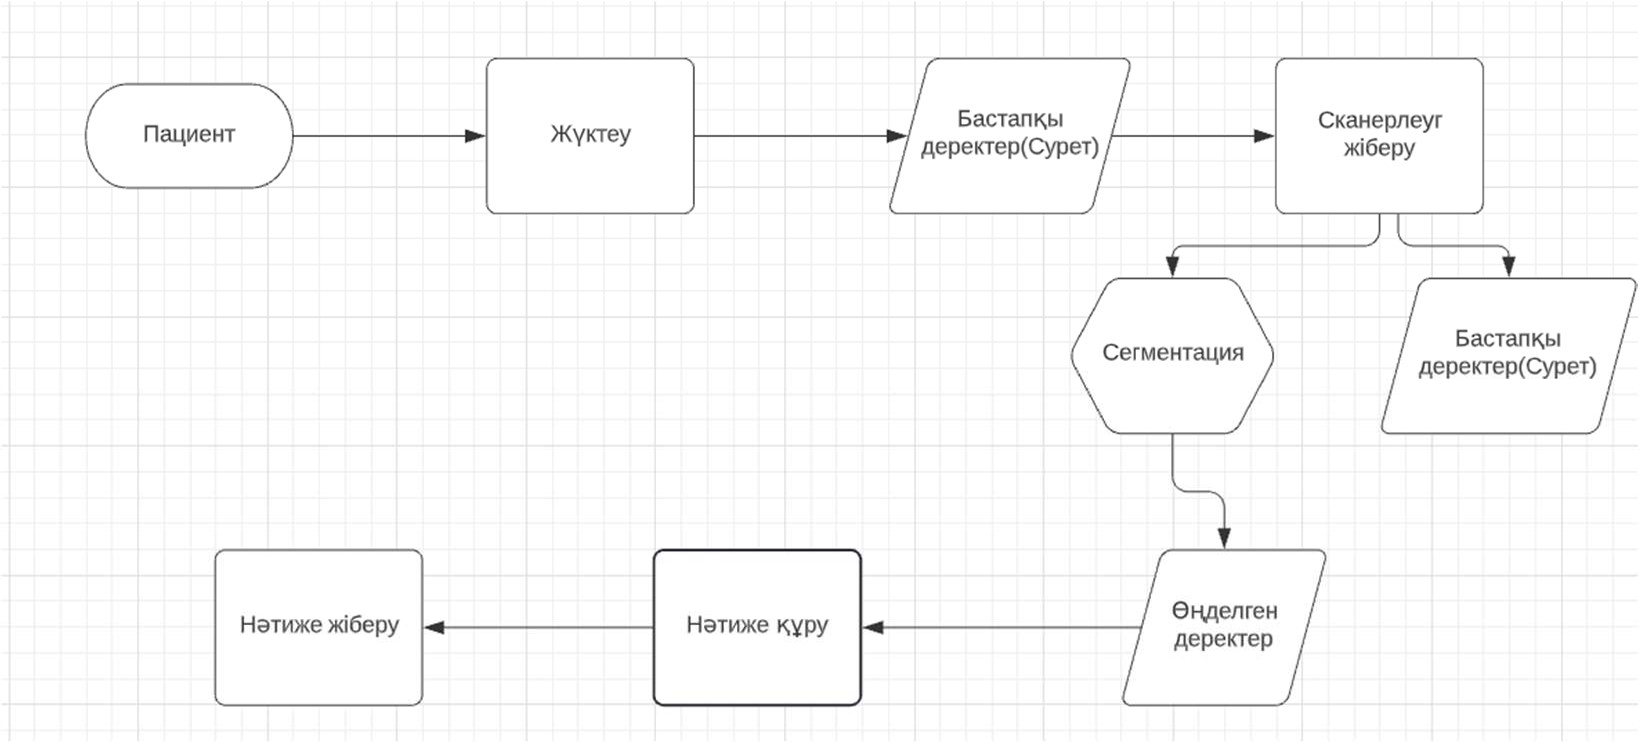
\includegraphics[width=0.8\textwidth]{assets/191}
	\caption*{}
\end{figure}

{\bfseries 1-сурет. Графикалық деректердің жүру картасы}

Деректер қорының негізгі кестелері бұл «қолданушылар» кестесі және де
өңдеуге арналған «деректер» кестесі болып табылады. Әр «қолданушы»
кестесіне арналған мәнге белгіле бір әдістер ие. Атап өтсек, бұл:
GetImage (); SetImage(); GetResult(); Download(). Төменде, 2-суретте
дизайн деңгейінде жүйені ұсынудың нұсқасы көрсетілген:

\begin{figure}[H]
	\centering
	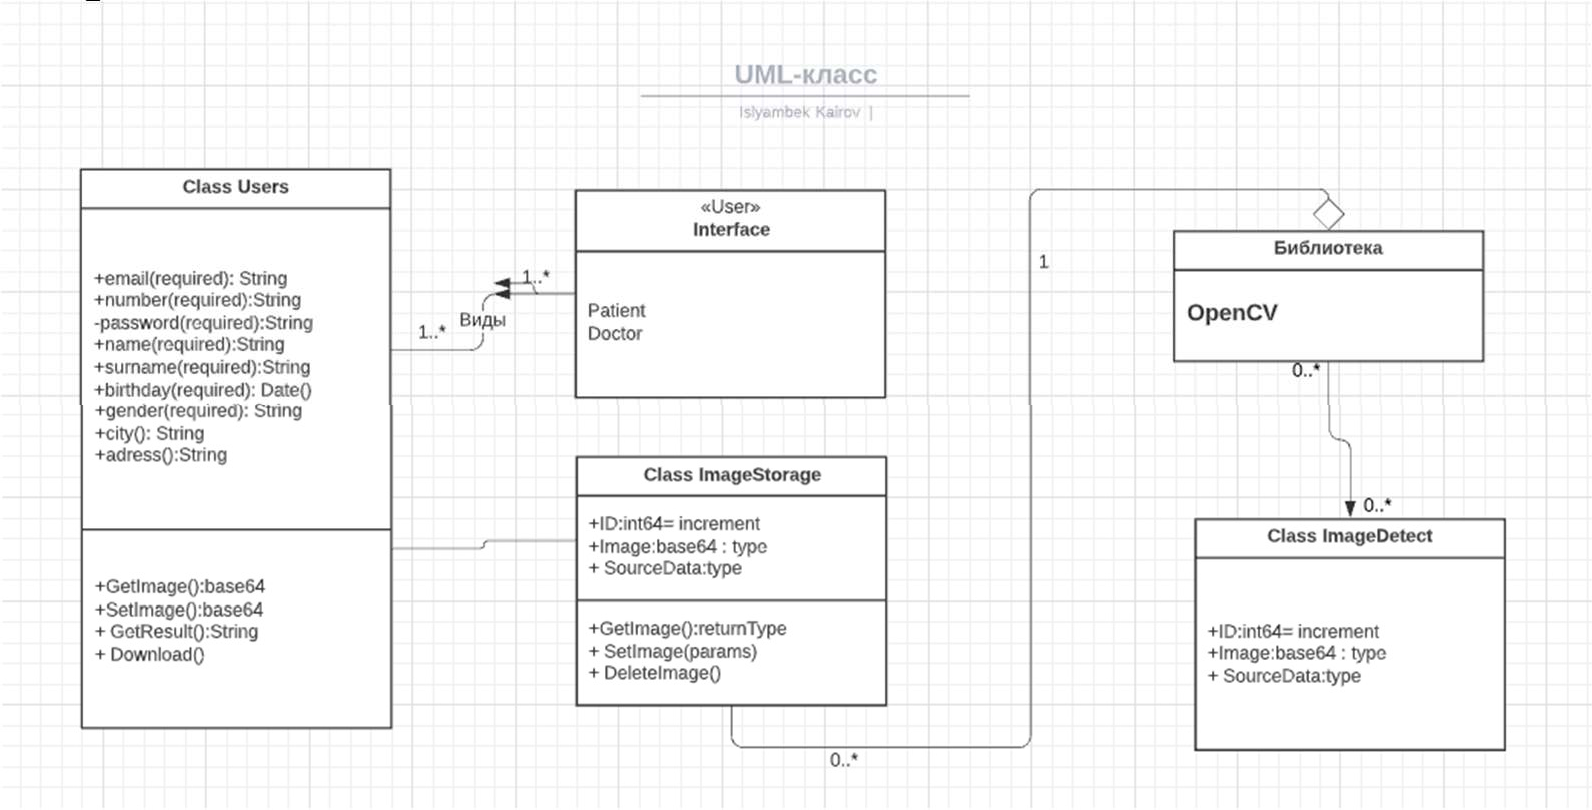
\includegraphics[width=0.8\textwidth]{assets/192}
	\caption*{}
\end{figure}

{\bfseries 2-сурет. Қолданушы және оған қатысты әдістердің мәндері}

Жүйе келесі негізгі функционалдық блоктардан тұрады: тіркеу,
аутентификация және авторизация, пайдаланушы үшін функционалдылық,
функционал дәрігер, кескін сегментациясының функционалдығы, бетті тану
кітапханасымен біріктіру функционалдығы, сканерлеу нәтижелері.

Жүйені іске асыру үшін келесі технологиялық стек ұсынылады.

Бэкенд: Язык NestJS, NodeJS, БД PostgreSQL.

Серверлік бөлім: Python, OpenCV, numpy.

Фронтенд: ReactNative, TypeScript.

Компьютерлік көруді жіктеудің жалпы проблемасы екі санатты (оқу деректер
жинағы мен сынақ деректер жинағы) ажырату болып табылады. Әдетте
компьютерлік көру тапсырмасы үшін істердің үлкен үлгісі пайдаланылды,
бірақ бұл оқу үшін біздің деректер жинағы шамамен екіге бөлінген 59
кескіннен тұрады, оның 29-ы сынақ үшін және 30-ы оқыту үшін. Деректер
Ұлттық денсаулық институттары {[}10{]} мақалаларынан жарияланған
медициналық суреттер онлайн OpenI репозиторийден алынған. Медицинадағы
цифрлық бейнелеу және коммуникациялар (DICOM) кескінді өңдеу үшін
кескіндерді импорттау, сандық форматқа түрлендіру үшін PyDicom Python
кітапханасы пайдаланылды. Caffe тәрізді басқа платформалармен пайдалану
алдында DICOM файлдарын PNG немесе Joint Photographic Experts Group
(JPEG) пішіміне түрлендіру мүмкін.

Tensorflow, Keras және Google Collab арқылы жүйесінде жазу кітапшалары
ұяшықтарға бөлінген және әрбір ұяшық өз бетінше жұмыс істей алады.
Блокнотта Keras кітапханасынан талаптары жүктелді {[}11{]}. Содан кейін
суреттер туралы ақпарат енгізілді. Соңында, дәуірлер санын (жаттығу
деректері арқылы өту саны) және партия өлшемін (бір уақытта өңделген
кескіндер саны) анықталды. Мембраналық мәліметтер жиынтығы (3-сурет):

\begin{figure}[H]
	\centering
	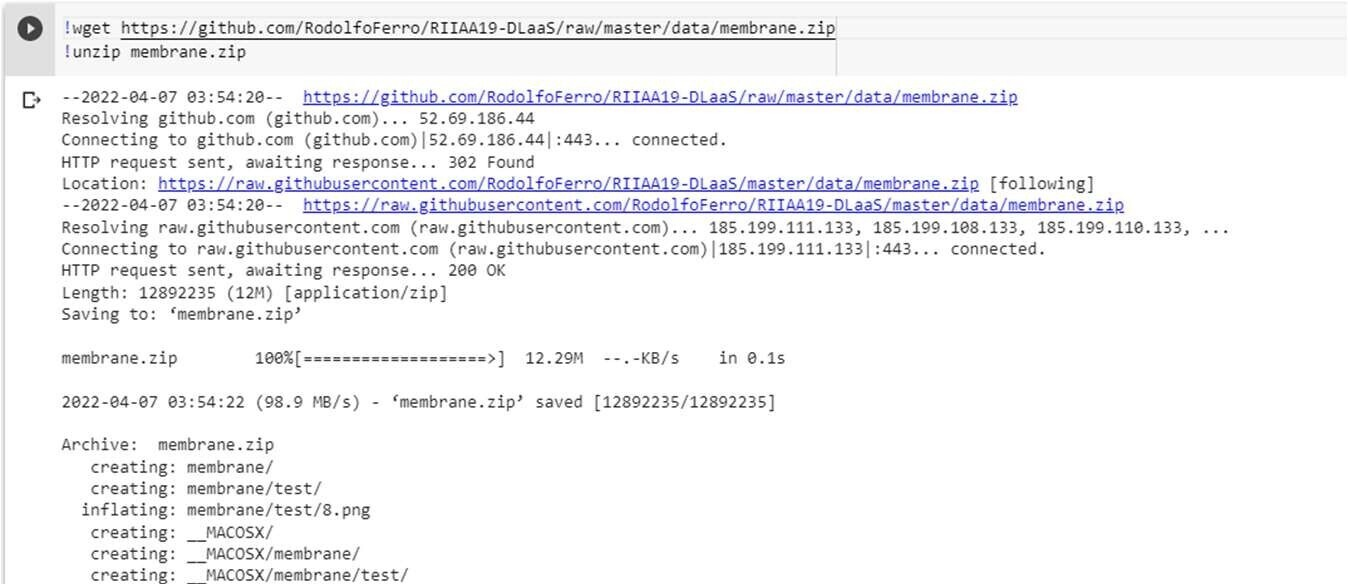
\includegraphics[width=0.8\textwidth]{assets/193}
	\caption*{}
\end{figure}

{\bfseries 3-сурет. Мембраналық мәліметтер жиынтығы}

Жүйенің модельдеу және жобалау функционалдығы толықтай зерттелді.

{\bfseries Нәтижелер мен талқылау.} Әзірленген қосымшаның негізгі
технологиясы -- жалпақ кескіндерді тану технологиясы болып табылады. Бұл
технология үшін әртүрлі кітапханалар бар. 4-суретте OpenCV кітапханасы
арқылы жасалған медициналық суреттің сегментация үлгісі көрсетілген.

% \begin{longtable}[]{@{}
%   >{\raggedright\arraybackslash}p{(\columnwidth - 2\tabcolsep) * \real{0.3983}}
%   >{\raggedright\arraybackslash}p{(\columnwidth - 2\tabcolsep) * \real{0.6017}}@{}}
% \toprule\noalign{}
% \begin{minipage}[b]{\linewidth}\raggedright
% \begin{figure}[H]
% 	\centering
% 	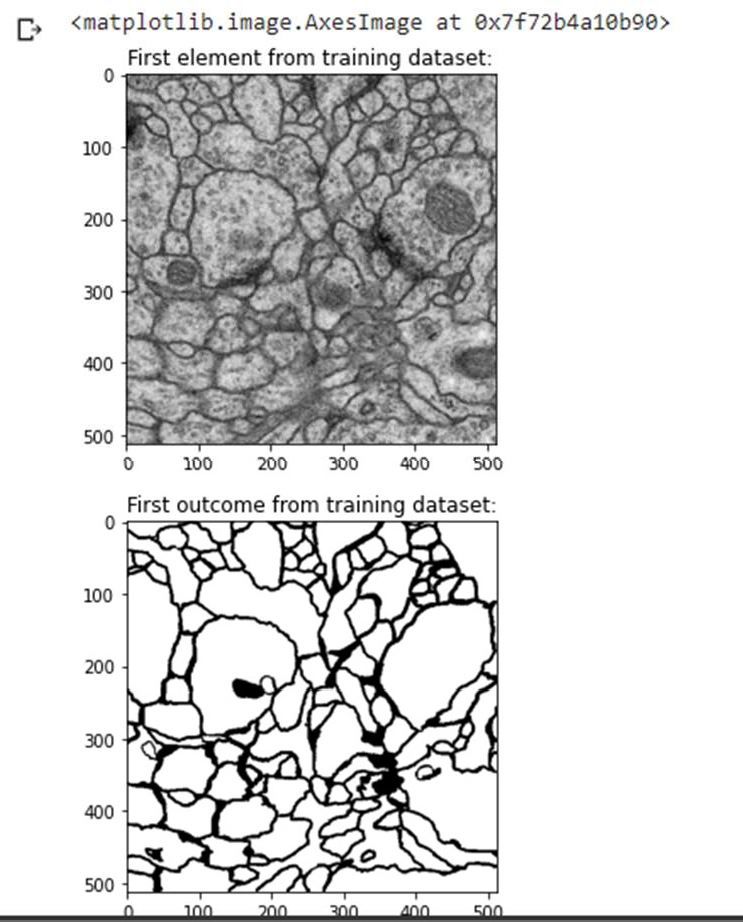
\includegraphics[width=0.8\textwidth]{assets/194}
% 	\caption*{}
% \end{figure}
% \end{minipage} & \begin{minipage}[b]{\linewidth}\raggedright
% \begin{figure}[H]
% 	\centering
% 	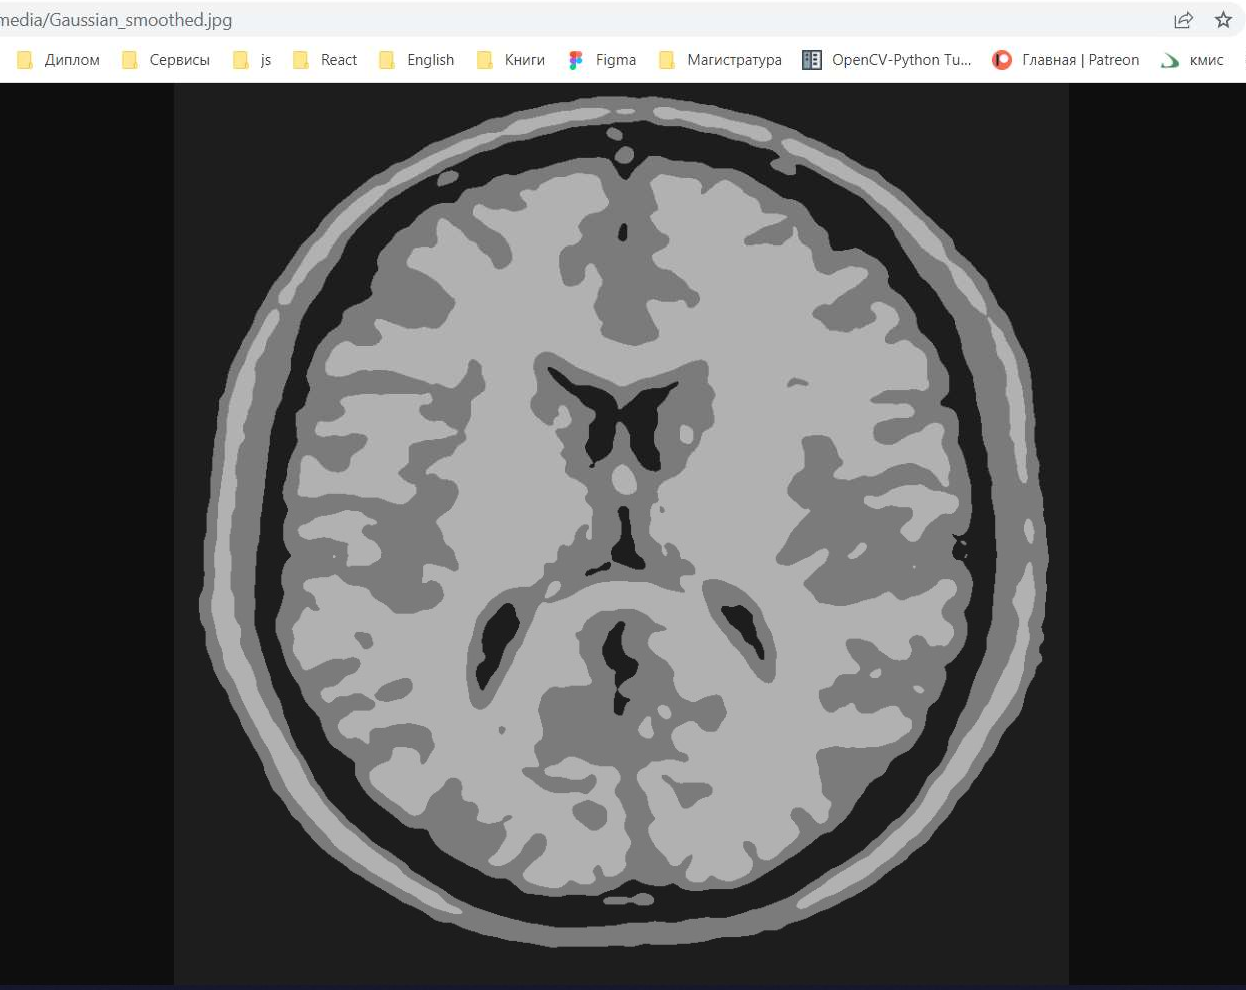
\includegraphics[width=0.8\textwidth]{assets/195}
% 	\caption*{}
% \end{figure}
% \end{minipage} \\
% \midrule\noalign{}
% \endhead
% \bottomrule\noalign{}
% \endlastfoot
% \multicolumn{2}{@{}>{\raggedright\arraybackslash}p{(\columnwidth - 2\tabcolsep) * \real{1.0000} + 2\tabcolsep}@{}}{%
% {\bfseries 4-сурет. Cегментация үлгісі}} \\
% \end{longtable}

Бұл зерттеуде серверлік бөлім ретінде Nest js программалық тілі
таңдалды. Сервер алдыңғы бөлігімен өзара әрекеттеседі, веб-параққа ұсыну
үшін деректерді береді және алады. Postman -- бұл басқалар жасаған
RESTful API-ді талдауға немесе өзіңіз жасаған API-ді тексеруге тырысудың
құралы (5-сурет). Тек маршрутты мекен-жай жолына қосу керек, сол жақтағы
ашылмалы тізімнен жауап алу әдісін таңдап, API кілтін «тақырыптар»
бөліміне енгізіп, «әдемі» JSON форматы шығады.

\begin{figure}[H]
	\centering
	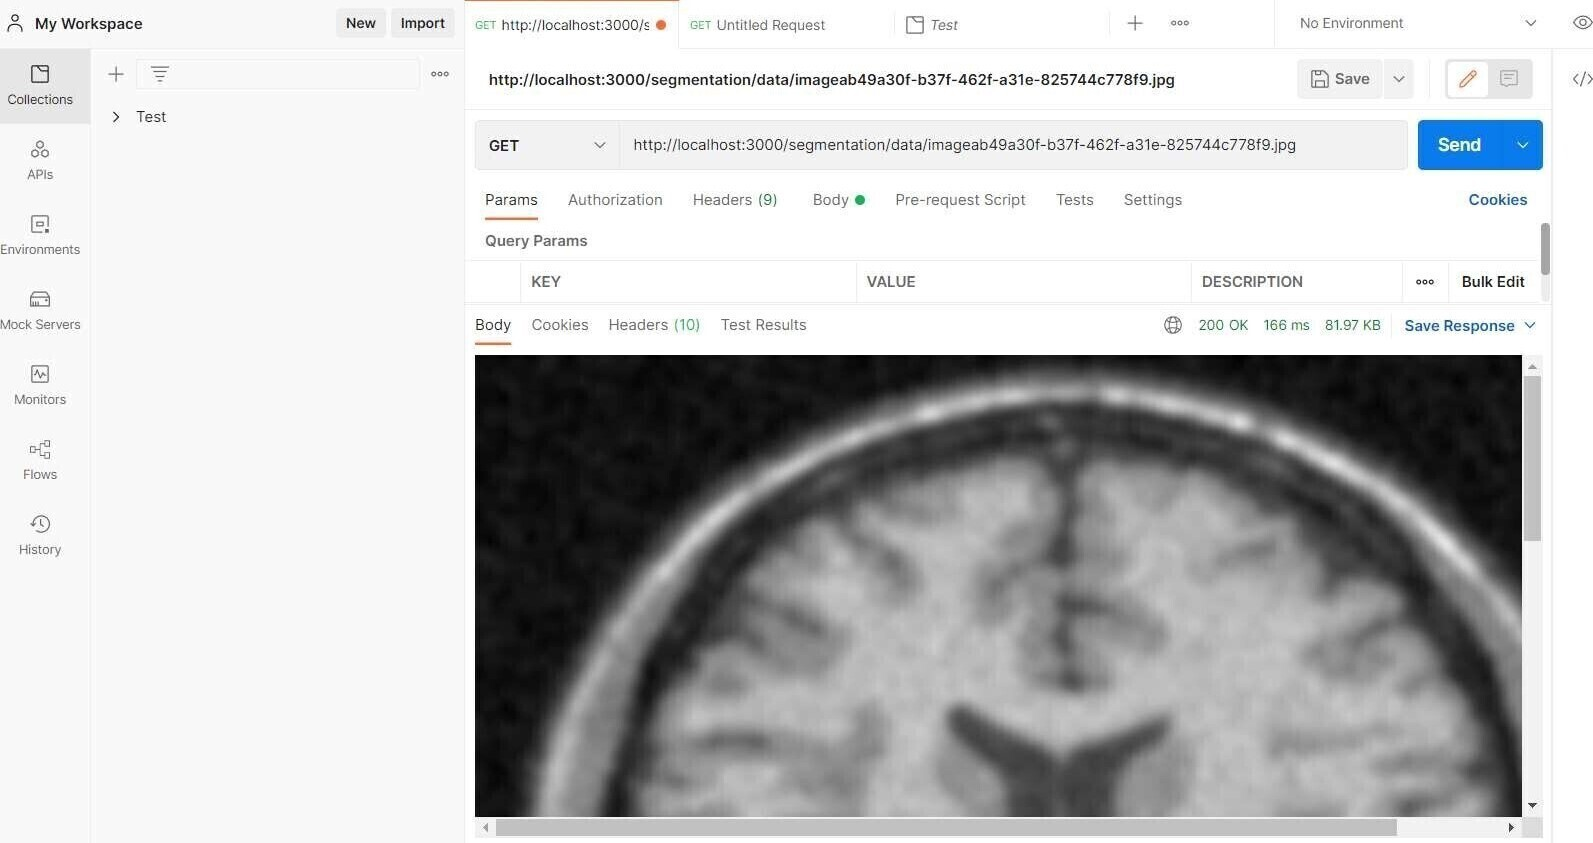
\includegraphics[width=0.8\textwidth]{assets/196}
	\caption*{}
\end{figure}

{\bfseries 5-сурет. Postman арқылы серверді тестілеу}

Осы зерттеуде PostgreSQL ДҚБЖ пайдаланылды. Келесі 6-суретте деректер
қорының негізгі кестелері сипатталған.

\begin{figure}[H]
	\centering
	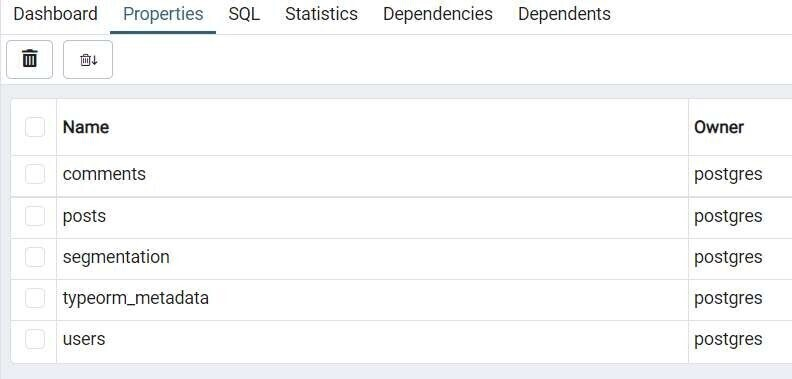
\includegraphics[width=0.8\textwidth]{assets/197}
	\caption*{}
\end{figure}

{\bfseries 6-сурет. Деректер қорының негізгі кестелері}

Клиенттік бөлім React Native Javascript кітапханасы технологиясы арқылы
жүзеге асырылған. Одан басқа мобильді қосымша құру кезінде келесі
қосымша кітапханалар орнатылды: Axios, Buffer,
@react-native-picker/picker, FontAwesome5,
@react-native-async-storage/async-storage, react-native-gesture-handler,
formik, @react-navigation/bottom-tabs, @react-navigation/stack,
@react-navigation/native. Қосымшаның демо нұсқасы Аndroid studio
программалық қамтама арқылы құрастырылады (7-сурет).

\begin{figure}[H]
	\centering
	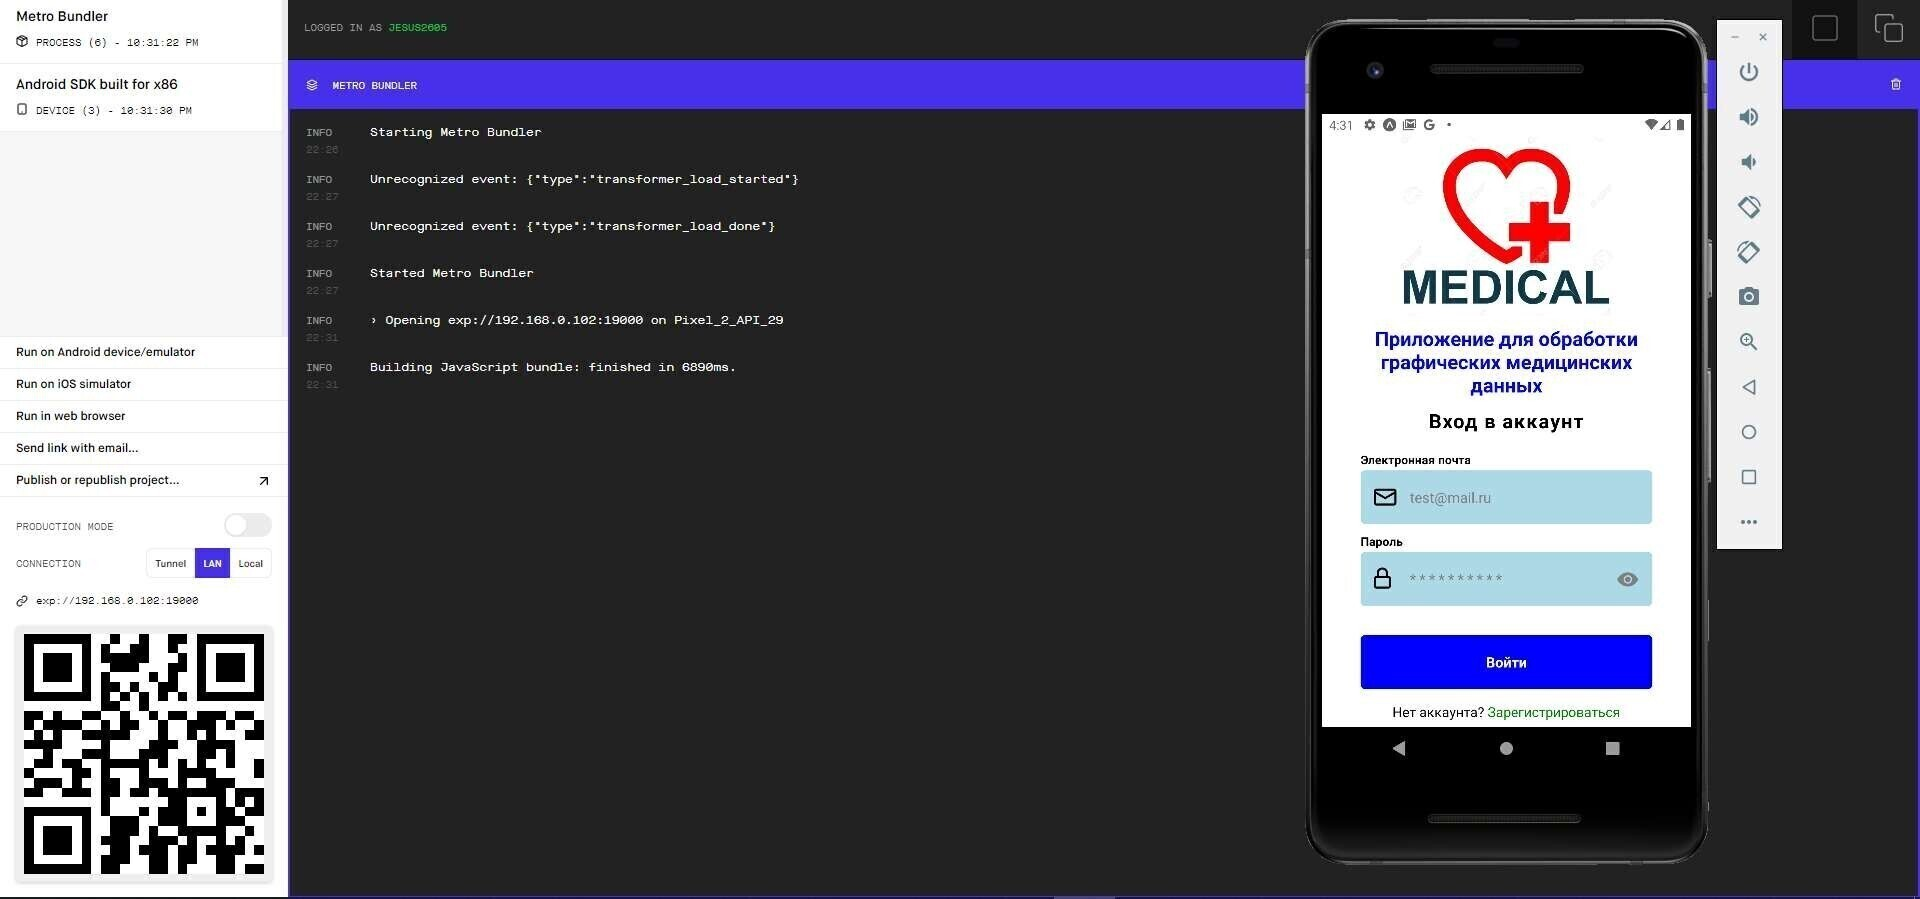
\includegraphics[width=0.8\textwidth]{assets/198}
	\caption*{}
\end{figure}

{\bfseries 7-сурет. Аndroid studio ортасында қосымшаның интерфейсі}

Жобаңың package.json файлы -- бұл қосымшамен өзара әрекеттесуде.
Виртуалды DOM тұжырымдамасы беретін абстракция дәрежесінің арқасында
React Native «көпір» жазуға тура келгенше басқа платформаларға назар
аудара алады.

{\bfseries Қорытынды.} Зерттеу жүргізу барысында программалық қосымша
арқылы медициналық кескіндерді сегментациялау жүзеге асырылды.
Медициналық кескіндерді сегментациялау әдістері зерттелінді. Әдістерді
толықтай талдап, артықшылықтары мен кемшіліктері анықталды. Әзірленген
жүйенің жобалау және модельдеуі сипатталды. Техникалық тапсырма кезінде
пайдаланушы, дәрігер және әкімші деген үш пайдаланушы түрі анықталды. Әр
пайдаланушы түріне бөлек функционал сипатталып, жасалынды. Жобада
қолданылған әр технология зерттелді. Практикада қолданылған келесі
технологиялар: Серверлік бөлім -- NestJS; Клиенттік бөлім --
ReactNative; Компьютерлік көру модулі -- OpenCV; Дерекқор базасы --
PostgresSQL. Программалық қамтамасыздандыру құру кезінде келесі
лицензияланған программаларды қолдандық: Visual Studio Code; Postman;
TablePlus; pgAdmin; ExpoGo. Осылайша, сегменттелген кескіндер
диагностиканың дәлдігін жақсартады, оларды пайдалануда, сақтауда және
одан әрі түсіндіруде ресурстарды үнемдейді. Мұндай қосымшалар үйден
шықпай-ақ бірнеше дәрігерден кеңес алуға мүмкіндік береді. Осы жерде
және қазір суретті оқудағы дәлдікті жақсартуға мүмкіндік беретін мұндай
қосымшаның Қазақстанда жұмыс істеуі басқа клиникалық тексеру әдістерімен
бірге орасан зор жетістік болуы мүмкін, өйткені ол дәрігер мен
пациенттің ортақ пікіріне жетуіне көмектеседі, нақты қорытынды жасалып,
кейіннен диагноз қойылады. Сондай-ақ, қолданбалы бұлтқа зерттеулердің
біраз көлемін сақтауға мүмкіндік беретін дерекқор базасы жасалынды және
кроссплатформалы қосымша құрылды. Құрылған мобильді қосымшаға толықтай
тестілеу жүргізілді. Қазақстандағы медицина саласында сәулелік
бейнелерді сегментациялау пациент диагнозын неғұрлым дәл диагностикалау
мен одан әрі верификациялау ең қажетті функцияларға айналуы мүмкін,
демек, әртүрлі ауруларды уақтылы анықтаудың арқасында халықтың өмір сүру
сапасын жақсартатын неғұрлым ұтымды және мақсатты емдеуге кең
қолданысына ие болады.

{\bfseries Әдебиеттер}

\begin{enumerate}
\def\labelenumi{\arabic{enumi}.}
\item
  Mei, H., Xu, K., Zhou, Y.~et al.~Camouflaged Object Segmentation with
  Omni Perception.~Int J Comput Vis. -2023. -Vol. 131. - P.3019-3034.
  https://doi.org/10.1007/s11263-023-01838-2
\item
  Маркелов, К. С. Модель повышения информативности цифровых изображений
  на базе метода суперразрешения / К.С. Маркелов // Инженерный вестники
  -- М. : ФГБОУ ВПО «МГТУ им. Н.Э. Баумана». -- 2013. -- Вып.3. -- С.
  525--542.
\item
  OpenCV tutorial. URL.
  https://medium.com/analytics-vidhya/opencv-tutorial-introduction-and-image-basics-7675866eb95a(өтініш
  берген күні: 9.03.2024)
\item
  Clarke LP, Velthuizen RP, Camacho MA, Heine JJ, Vaidyanathan M, Hall
  LO, Thatcher RW, Silbiger ML. MRI segmentation: methods and
  applications. Magn Reson Imaging.-1995. -Vol. 13(3). -P.343-368. doi:
  10.1016/0730-725x(94)00124-l. PMID: 7791545.
\item
  Chaohui Wang, Nikos Komodakis, Nikos Paragios. Markov Random Field
  modeling, inference \& learning in computer vision \& image
  understanding//A survey, Computer Vision and Image Understanding.
  -2013. -Vol. 117. Iss. 11. -P. 1610-1627.
  https://doi.org/10.1016/j.cviu.2013.07.004.
\item
  Modernizing Computer Vision with the Help of Neural Networks.
  {[}URL{]}. - https://marutitech.com/computer-vision-neural-networks/
  (өтініш берген күні: 9.03.2024)
\item
  Шуйтенов, Г., У.~Турусбекова, М.~Муратбеков Анализ научных текстов на
  основе языковых моделей алгоритмами распределенной обработки// Вестник
  КазУТБ -2023. -№4(21). doi:10.58805/kazutb.v.4.21-220.
\item
  McInerney T, Terzopoulos D. Deformable models in medical image
  analysis: a survey. Published in Medical Image Analysis. -1996.
  -Vol.1(2). -P. 91-108.
  https://web.cs.ucla.edu/\textasciitilde dt/papers/mia96/mia96.pdf
\item
  An end-to-end platform for machine learning: Get started with
  TensorFlow https://www.tensorflow.org/?hl=ru (өтініш берген күні:
  12.03.2024)
\item
  Open Access Biomedical Image Search Engine. https://openi.nlm.nih.gov.
  (өтініш берген күні: 15.03.2024)
\item
  Декодирование файлов DICOM для получения медицинских изображений.
  https://www.tensorflow.org/io/tutorials/dicom (өтініш берген күні:
  15.03.2024)
\end{enumerate}

{\bfseries References}

1. Mei, H., Xu, K., Zhou, Y. et al. Camouflaged Object Segmentation with
Omni Perception. Int J Comput Vis. -2023. -Vol. 131. - P.3019-3034.
https://doi.org/10.1007/s11263-023-01838-2

2. Markelov, K. S. Model\textquotesingle{} povyshenija informativnosti
cifrovyh izobrazhenij na baze metoda superrazreshenija / K.S. Markelov
// Inzhenernyj vestniki -- M. : FGBOU VPO «MGTU im. N.Je. Baumana». --
2013. -- Vyp.3. -- S. 525--542. {[}in Russian{]}

3. OpenCV tutorial. URL.
https://medium.com/analytics-vidhya/opencv-tutorial-introduction-and-image-basics-7675866eb95a(date
of application: 9.03.2024)

4. Clarke LP, Velthuizen RP, Camacho MA, Heine JJ, Vaidyanathan M, Hall
LO, Thatcher RW, Silbiger ML. MRI segmentation: methods and
applications. Magn Reson Imaging.-1995. -Vol. 13(3). -P.343-368. doi:
10.1016/0730-725x(94)00124-l. PMID: 7791545.

5. Chaohui Wang, Nikos Komodakis, Nikos Paragios. Markov Random Field
modeling, inference \& learning in computer vision \& image
understanding//A survey, Computer Vision and Image Understanding. -2013.
-Vol. 117. Iss. 11. -P. 1610-1627.
https://doi.org/10.1016/j.cviu.2013.07.004.

6. Modernizing Computer Vision with the Help of Neural Networks.
{[}URL{]}. - https://marutitech.com/computer-vision-neural-networks/
(date of application: 9.03.2024)

7. Shujtenov, G., U. Turusbekova, M. Muratbekov Analiz nauchnyh tekstov
na osnove jazykovyh modelej algoritmami raspredelennoj obrabotki//
Vestnik KazUTB -2023. -№4(21). doi:10.58805/kazutb.v.4.21-220. {[}in
Russian{]}

8. McInerney T, Terzopoulos D. Deformable models in medical image
analysis: a survey. Published in Medical Image Analysis. -1996.
-Vol.1(2). -P. 91-108.
https://web.cs.ucla.edu/\textasciitilde dt/papers/mia96/mia96.pdf

9. An end-to-end platform for machine learning: Get started with
TensorFlow https://www.tensorflow.org/?hl=ru (date of application:
12.03.2024)

10. Open Access Biomedical Image Search Engine.
https://openi.nlm.nih.gov. (date of application: 15.03.2024)

11. Dekodirovanie fajlov DICOM dlja poluchenija medicinskih
izobrazhenij. https://www.tensorflow.org/io/tutorials/dicom (date of
application: 15.03.2024)

\emph{{\bfseries Авторлар туралы мәліметтер}}

Есенгалиева Ж.С. - PhD, доцент м.а., Л.Н. Гумилев атындағы Еуразия
ұлттық университеті, Астана, Қазақстан,

е-mail:jannayess@gmail.com;

Оралбекова Ж.О. - PhD, доцент, Л.Н. Гумилев атындағы Еуразия ұлттық
университеті, Астана, Қазақстан,

е-mail:oralbekova@bk.ru;

Турарова М.К. - PhD, Л.Н. Гумилев атындағы Еуразия ұлттық университеті,
Астана, Қазақстан,

е-mail:marzhan\_08@mail.ru

\emph{{\bfseries Information about the authors}}

Yessengaliyeva Zh.S. - PhD, аcting associate professor, Eurasian
national university, Astana, Kazakhstan,

е-mail:jannayess@gmail.com;

Oralbekova Zh.O. - PhD, associate professor, Eurasian national
university, Astana, Kazakhstan,

е-mail:oralbekova@bk.ru;

Turarova M.K. - PhD, Eurasian national university, Astana, Kazakhstan,
е-mail:marzhan\_08@mail.ru\newpage
{\bfseries МРНТИ 81.93.29}

{\bfseries ЗАТТАР ИНТЕРНЕТІ ҚҰРЫЛҒЫЛАРЫНЫҢ ҚАУІПСІЗДІГІН ҰЙЫМДАСТЫРУДА
ФЕДЕРАТИВТІ ОҚЫТУ ӘДІСТЕРІН ҚОЛДАНУ}

{\bfseries \textsuperscript{1}А. Адамова\textsuperscript{🖂},
\textsuperscript{1,2}Т. Жукабаева}

\textsuperscript{1}Astana IT University, Астана, Қазақстан,

\textsuperscript{2}Л.Н. Гумилев атындағы Еуразиялық ұлттық университеті,
Астана, Қазақстан

{\bfseries \textsuperscript{🖂}}Корреспондент-автор:
aigul.adamova@astanait.edu.kz

Заттар интернеті құрылғыларының өзара әрекеттесуінің негізгі
технологияларының бірі болып табылады. Заттар интернеті құрылғыларының
өзара әрекеттесуі кезінде ресурстардың белгілі шектеулері бар. Бұл
шектеулер заттар интернеті құрылғыларының нақты уақыт режиміндегі өзара
әрекеттесуіне әсер етеді және желіні пайдаланушылардың жеке деректерінің
қауіпсіздігі мәселесіне әсерін береді. Бұл жұмыс заттар интернеті
құрылғыларының қауіпсіздігін арттыру мақсатында, машиналық оқытудың
иновациялық әдісі болып табылатын -- федеративті оқытудың қолданылуын
зерттеу туралы. Мақалада федеративті оқытудың әлемдік зерттеулерде
қолданылуы туралы шолу келтірілген. Федеративті оқытудың ``Federative
average'' әдісі көмегімен тоғыз заттар интернеті құрылғыларының өзара
әрекеттесуі барысында алынған желілік трафик бойынша DDoS щабуылын
анықтау жолы талданған. Нәтижесінде бағалау көрсеткіштері арқылы ұсынған
жүйенің қолданылуы бағаланды.

{\bfseries Түйін сөздер}: Заттар интернеті, қауіпсіздік, желілік шабуылдар,
машиналық оқыту, федеративті оқыту, DDoS

{\bfseries ОБЕСПЕЧЕНИЕ БЕЗОПАСНОСТИ УСТРОЙСТВ ИНТЕРНЕТ ВЕЩЕЙ}

{\bfseries С ПОМОЩЬЮ МЕТОДОВ ФЕДЕРАТИВНОГО ОБУЧЕНИЯ}

{\bfseries \textsuperscript{1}А. Адамова\textsuperscript{🖂},
\textsuperscript{1,2}Т. Жукабаева}

\textsuperscript{1}Astana IT University, Астана, Казахстан,

\textsuperscript{2}Евразийский национальный университет им. Л. Н.
Гумилева, Астана, Казахстан

е-mail: aigul.adamova@astanait.edu.kz

Интернет вещей является одной из основных технологий взаимодействия
устройств. При взаимодействии устройств Интернета вещей существуют
определенные ограничения ресурсов. Эти ограничения влияют на
взаимодействие устройств Интернета вещей в режиме реального времени и
влияют на проблему безопасности личных данных пользователей сети.
Представленная работа посвящена изучению использования федеративного
обучения который является инновационным подходом машинного обучения, с
целью повышения безопасности устройств Интернет вещей. В статье
представлен обзор использования федеративного обучения в мировых
исследованиях. С помощью метода федеративного обучения ``Federative
average'' анализируется сетевой трафик, полученный при взаимодействии
девяти устройств Интернет вещей на выявление DDoS атак. В результате
оценивалось применение предложенной системы с помощью оценочных
показателей.

{\bfseries Ключевые слова:} Интернет вещей, безопасность, сетевые атаки,
машинное обучение, федеративное обучение, DDoS атака

{\bfseries ENSURING THE SECURITY OF INTERNET OF THINGS DEVICES USING}

{\bfseries FEDERATED LEARNING METHODS}

{\bfseries \textsuperscript{1}А. Аdamova\textsuperscript{🖂},
\textsuperscript{1,2}Т. Zhukabayeva}

\textsuperscript{1}Astana IT University, Astana, Kazakhstan,

\textsuperscript{2} L.N. Gumilyov Eurasian National University, Astana,
Kazakhstan

е-mail: aigul.adamova@astanait.edu.kz

The Internet of Things (IoT) is one of the key technologies for device
interaction. However, there are certain resource limitations in IoT
device interactions. These limitations impact real-time interactions of
IoT devices and pose challenges to the security of
users\textquotesingle{} personal data within the network. This work
explores the use of federated learning, an innovative machine learning
approach, to enhance the security of IoT devices. The article provides
an overview of the use of federated learning in global research. The
federated learning method \textquotesingle Federated
Average\textquotesingle{} is used to analyze network traffic generated
by the interaction of nine IoT devices to detect DDoS attacks. The
proposed system was evaluated using performance metrics.

{\bfseries Key words}: Internet of Things, security, network attack,
machine learning, federated learning, DDoS.

{\bfseries Кіріспе.} Қазіргі таңда өнеркәсіптің және адамның күнделікті
қызмет салаларының сандық трансформациялануы, 4.0 Индустриясының,
сенсорлы және пилотсыз технологиялардың дамуы, физикалық үрдістерді
өзара ақпаратпен алмасу арқылы іске асыратын Интернет заттардың
(Internet of Things, IoT) кең таралуына себеп болды. Күн сайын үлкен
көлемдегі деректерді жинауға және тасымалдауға қабілетті жаңа құрылғылар
шығарылуда. IoT құрылғылары түрлі деректерді жинайды, олардың ішінде
жеке ақпарат, құпия немесе қауіпсіздікпен байланысты ақпарат. IoT
құрылғылар санының қарқынды өсуі - ақпараттың қауіпсіздігі мен
құпиялылығына байланысты жаңа мүмкіндіктермен қатар, үлкен қиындықтарды
тудырады. Бұл кеңейіп келе жатқан экожүйенің қауіпсіздігі мен
сенімділігін қамтамасыз ету үшін, бұл мәселелерді түбегейлі шешу қажет.
Үлкен деректер, IoT құрылғыларының алуан түрі көптеген шабуылдарға тап
болуы жаңалық емес. IoT құрылғыларымен жиналатын деректерге рұқсатсыз
қол жеткізу қаржылық шығындарға, физикалық қауіпке және түрлі
зардаптарға әкелуі мүмкін. 2016 жылы қауіпсіздік камерасының белгілі бір
үлгісінде осалдылық табылып, 300 мыңға жуық IoT бейнежазба жүргізетін
құрығылар арқылы Spotify, Reddit сияқты әлеуметтік желілерге шабуылдар
жасалған {[}1{]}. 2019 жылы Wyze Labs Inc. компаниясы ақылды үй
қауіпсіздік жүйесінің бұзылғаны туралы хабарланған, онда 2,4 миллионға
жуық қолданушылардың жеке мәліметтерінің құпиялылығы сақталмаған
{[}2{]}. Онымен қатар, 2024 жылдың ақпан айында Wyze Labs ақылды үйге
арналған камера өндіруші компаниясы өз қолданышуларына қызмет көрсетуін
тоқтатуға мәжбүр болды. 13000 қолданушыға қатысты емес, басқа ақылды
үйлердің бейнежазба деректері келіп түскен. Бұл жағдай желілік
хаттамалар осалдылық салдарынан орын алды {[}3{]}. IoT құрылғыларының
өзара әрекеттесу барысында ақпараттың құпиялылығын сақтау, аталған
жағдайлардың қайталанбауы немесе оларды алдын алу - қазіргі таңда өзекті
мәселелердің бірі болып келеді.

IoT құрылғыларының ақпараттық қауіпсіздігін ұйымдастыру бойынша, бүгінгі
күні, танымал әдістердің негізін құрайтын машиналық оқыту әдістері кең
қолданылуда. IoT қауіпсіздігін ұйымдастыру барысында K-Nearest Neighbor,
Artificial Neural Network, Support Vector Machine, Decision Tree, Random
Forest, Logistic Regression және тағы көптеген машиналық оқытудың
әдістерінің қолданылу аясы ауқымды {[}4{]}. Машиналық оқыту әдістері
жиналған деректерді талдай отырып, қалыпты жағдайдан ауытқуларды нақты
уақыт режимінде анықтап, қауіптерді болжай алады {[}5{]}. Дәстүрлі
Машиналық оқыту әдістері көбінесе орталықтандырылған серверде үлкен
көлемдегі деректерді жинау мен оларды талдау үрдістерін қамтиды
{[}6,7{]}. Дегенмен, бұл тәсіл құпиялылық тұрғысынан деректер
қауіпсіздігінің бұзылуы, жеке деректерді қорғау туралы қатаң заңдардың
болуы, сенімсіздіктің болуы сияқты бірқатар қиындықтарды тудырады.
Ұсынылып отырған мақалада IoT құрылғылар рөлінің артуы, құпия
деректердің маңыздылығына байланысты ақпараттың құпиялылығын сақтауға
және бір уақытта модельдердің жоғары дәлдігін қамтамасыз етуге мүмкіндік
беретін машиналық оқытудың жаңа тәсілі - федеративті оқыту зерттеледі.

Федеративті оқыту - модельді үлестірілген деректер негізінде оқытатын
машиналық оқытудың нновациялық әдісі болып келеді {[}8{]}. Бұл жағдайда
деректер орталық серверде жиналмайды, онымен қоса аталған әдіс -
деректер құпия болған жағдайда аса пайдалы болып келеді {[}9{]}.
Федеративті оқыту негізіндегі әдістер дәстүрлі орталықтандырылған
машиналық оқыту нұсқаларымен салыстырғанда - қолданышулардың жеке
деректерінің құпиялығын сақтауда және шабуылды анықтау нақтылығында
жоғары көрсеткішті шешімдер көрсетеді {[}10{]}. Жеке деректердің
құпиялығы мен жүйенің сенімділігін арттыру мақсатында федеративті
оқытуды блокчейн технологиясымен IoT жүйелерінде аномалияны анықтау үшін
қолданады {[}11{]}. IoT құрылғыларының ресурстарының жетіспеушілігі
шектелген есептеу қабілеті, төмен өткізгіштік қабілеті, төмен қуаттылығы
және шектелген жадыға байланысты. осыған байланысты, IoT құрылғылары
үшін үлестірілген машиналық оқыту жолдары қз қолданысын тапқан болатын
{[}12{]}. Сайып келгенде, федеративті оқыту тәсілінің IoT құрылғылары
желісінде жеке деректердің құпиялығын сақтаудағы перспективасы анық.
Жұмыс барысында IoT құрылғылар желісіндегі Ddos шабуылын анықтау үшін
федеративті оқыту әдісі негізіндегі жүйе ұсынылады. Федеративті оқыту
мен деректерді талдау үйлесімі пайдаланушылардың құпиялылығын бұзбай,
DdoS шабуылдарымен тиімді күресуге мүмкіндік береді. Бұл қауіпсіз және
сенімді заттар интернетін дамытудың жаңа мүмкіндіктерін ашады.

{\bfseries Материалдар мен әдістер.} IoT жүйелерінің дәстүрлі үш деңгейлі
архитектурасы қарастыратын болсақ, әрбір деңгейге тән қауіпсіздік
қатерлерін байқауға болады. Қауіпсіздік қатерлері жеке деректердің
бұзылуына әкеледі {[}13{]}. Үш деңгейлі архитектурасы қосымша, желілік
және сенсорлық деңгейлерден тұрады {[}14{]}. Сенсорлы деңгейдегі
шабуылдар рұқсатсыз кіру немесе бақылау үшін, құрылғының
микробағдарламасындағы әлсіз жерлерді пайдалану арқылы, құпия ақпаратты
алу үшін құрылғылардың физикалық сипаттамаларын талдау арқылы,
құрылғыларға рұқсатсыз кіру үшін ұрланған тіркелгі деректерін пайдалану
арқылы, өндіріс процесіне зиянды компоненттерді немесе бағдарламалық
жасақтаманы енгізу арқылы жасала алады {[}15{]}. Желілік деңгейдегі
шабуылдар ретінде құрылғылар мен шлюз арасындағы байланысты ұстап алу
және басқару арқылы асырылатын MITM немесе шлюзді қол жетімсіз ету үшін
трафиктің шамадан тыс жүктелуін атауға болады {[}16{]}. Қосымша
деңгейіндегі шабуылдар ретінде SQL инъекция арқылы шекті деректерге қол
жеткізу сияқты жағдайларды атауға болады {[}17{]}. Барлық шабуылдар IoT
желісіне үлкен қауіп төндіреді. Осы қауіпті алдын алу алу үшін
федеративті оқытудың IoT қауіпсіздігін ұйымдастыру барысында қолданылуы
туралы соңғы жылдары зерттеген жұмыстарға талдау жасалды. Талдау
нәтижесі 1-кестеде ұсынылған.

{\bfseries 1-кесте. Федеративті оқытудың IoT қауіпсізідігінде қолданылған
жұмыстарға шолу}

\begin{longtable}[]{@{}
  >{\raggedright\arraybackslash}p{(\columnwidth - 6\tabcolsep) * \real{0.1156}}
  >{\raggedright\arraybackslash}p{(\columnwidth - 6\tabcolsep) * \real{0.1094}}
  >{\raggedright\arraybackslash}p{(\columnwidth - 6\tabcolsep) * \real{0.3812}}
  >{\raggedright\arraybackslash}p{(\columnwidth - 6\tabcolsep) * \real{0.3938}}@{}}
\toprule\noalign{}
\endhead
\bottomrule\noalign{}
\endlastfoot
Мақала & жылы & Негізгі мазмұны & Федеративті оқытудың қолданылуы \\
{[}18{]} & 2024 & Авторлар қауіпсіз және тиімді IoT жүйелерін құру үшін
кванттық есептеулердің, Федеративті оқытудың және 6g желілерінің
тұжырымдамалық интеграциясын ұсынған. & Федеративті оқыту IoT
құрылғыларына құпиялылықты қорғау үшін орталық серверге деректерді
жібермей модельдерді бірлесіп оқытуға мүмкіндік береді. \\
{[}19{]} & 2024 & Автор түрлі шабуылдарды анықтауда дәстүрлі
орталықтандырылған әдістері ауқымды және әртүрлі IoT желілерінде тиімсіз
екенін атап, федеративті оқытуға негізделген жаңа тәсіл ұсынған. &
Федеративті оқыту конволюциялық нейронды желілерді пайдаланып DDoS
шабуылдарды тиімді анықтауға көмектеседі. \\
{[}20{]} & 2024 & Мақала Машиналық оқыту алгоритмдерін қолдана отырып,
IoT құрылғы хосттарындағы түрлі шабуылдардың жіктелуін ұсынады. & Tree
decision, Lite Gradient Boost, Xtra Gradient Boost және Random Forest,
сияқты Машиналық оқыту алгоритмдерінің ансамбльдері жоғары дәлдікті
қамтамасыз етеді. \\
{[}21{]} & 2020 & Жұмыста федеративті оқыту барысында қауіпсіздік пен
сенімділіктің қатерлері зерттеледі & Федеративті оқыту әрбір қолданышуға
модельді жергілікті түрде оқытуға мұмкіндік береді және
орталықтандаралған серверде жаһандық агрегация жасалады \\
{[}22{]} & 2022 & Мақалада киберқауіпсіздік бойынща деректер жинағы
ұсынылған & машиналық оқыту әдістерінің тиімділігі федеративті оқыту
режимінде бағаланған \\
{[}23{]} & 2022 & Жұмыста федеративті оқыту негізінде құрастырылған жаңа
алгоритм ұсынылған & Федеративті оқытудың негізгі кемшіліктерін
зерттейді. \\
{[}24{]} & 2023 & жұмыс жоғары дәлдіктегі және деректердің құпиялылығын
қорғауды күшейтетін IoT құрылғыларындағы кибершабуылдарды анықтау үшін
FL және көп қабатты перцептронды нейрондық желілерді пайдаланатын хост
негізіндегі кіруді анықтау жүйесін ұсынады. & Федеративті оқыту IoT
құрылғыларының қауіпсіздігін жақсарту үшін қолданылады \\
{[}25{]} & 2023 & Жұмыстағы ұсынылған әдіс иерархиялық құрылымды,
адаптивті деректерді қысу алгоритмін және IOT құрылғылары мен Орталық
сервер арасындағы тиімді, қауіпсіз және құпия өзара әрекеттесу үшін
SEP-IoT хаттамасын қамтиды & Федеративті оқыту IoT жүйелеріндегі
қауіпсіздік пен құпиялылықты арттыру үшін қолданылады \\
{[}26{]} & 2023 & Мақалада FLIP 4 жергілікті IoT құрылғыларындағы
машиналық оқыту үлгілерін оқытуға мүмкіндік беретін әдіс зерттеледі &
FLIP 4-федеративті оқытуға негізделген IoT желісіндегі шабуылдарды
анықтауға арналған платформа \\
\end{longtable}

Осы зерттеу бағытындағы 1-кестеде келтірілген мақалаларды талдай отырып,
федеративті оқыту әдісі - деректерді жергілікті құрылғыларда сақтауға,
дәстүрлі машиналық оқытуға тән шығындарды және өнімділік кедергілерін
азайту арқылы IoT құрылғыларының қауіпсіздігін арттыра алатынына көз
жеткізуге болады. Ол сондай-ақ есептеу және желі шығындарын азайтады,
қауіпсіздік пен құпиялылықты арттырады, параллелизацияны пайдаланады
және смарт жүйелердің тұрақтылығын арттырады. Негізі федеративті
оқытудың FedAvg, FedProx сияқты түрлі алгоритмдері бар. Бұл жұмыста
FedAvg (Federated Averaging) алгоритмін IoT құрылғыларымен жиналған
деректер қорында Ddos шабуылдарды анықтау мақсатымен қолданылады. DDoS
шабуылдары компанияның немесе ұйымның беделіне айтарлықтай зиян келтіруі
мүмкін. DDoS шабуылдарының негізгі мақсаты - интернеттегі кез-келген
ресурсты қол жетімсіз ету. Бұл ұйымдар үшін үлкен қаржылық шығындарға
және пайдаланушылар үшін қолайсыздықтарға әкелуі мүмкін.

FedAvg -- федералды оқытудың ең танымал алгоритмдерінің бірі. Бұл әр
құрылғыда жергілікті деректерді сақтай отырып, көптеген құрылғыларда
машиналық оқыту модельдерін оқытуға мүмкіндік береді {[}27{]}. Алгоритм
8 қадамнан тұратын орындалу үрдісі 1-суретте көрсетілген. Алғашқы
қадамында орталық сервер жаһандық модельді инициализацияласа, келесі
оқыту қадамына қатысу үшін қолданушылардың ішкі жиыны таңдалады. Бұл
таңдау ерікті немесе стандарттар жиынтығымен анықталады. Кейін таңдалған
қолданушылар жаһандық үлгіні алады. Модель әр клиенттік құрылғыда
жергілікті деректерді қолдана отырып оқытылады. Модельдің өнімділігін
арттыру мақсатында көптеген итерацияларды немесе түрлі уақыт аралықтары
қамтылуы мүмкін. Келесі қадамда, әрбір клиенттен оқытылған жаңа
модельдер орталық серверге жіберліді. Орталық сервер, клиенттерден
алынған модельдерді - модель параметрлерін орташалау арқылы біріктіреді.
Бұл орташалау процесі жаһандық модельдің құпиялығын сақтай отырып,
әртүрлі қоланушылардан алған ақпараттың пайдалылығын қамтамасыз етеді.
Клиентті таңдау және модельді орташалау арасындағы қадамдар қажетті
өнімділік деңгейіне жеткенше дейін қайталана алады.

\begin{figure}[H]
	\centering
	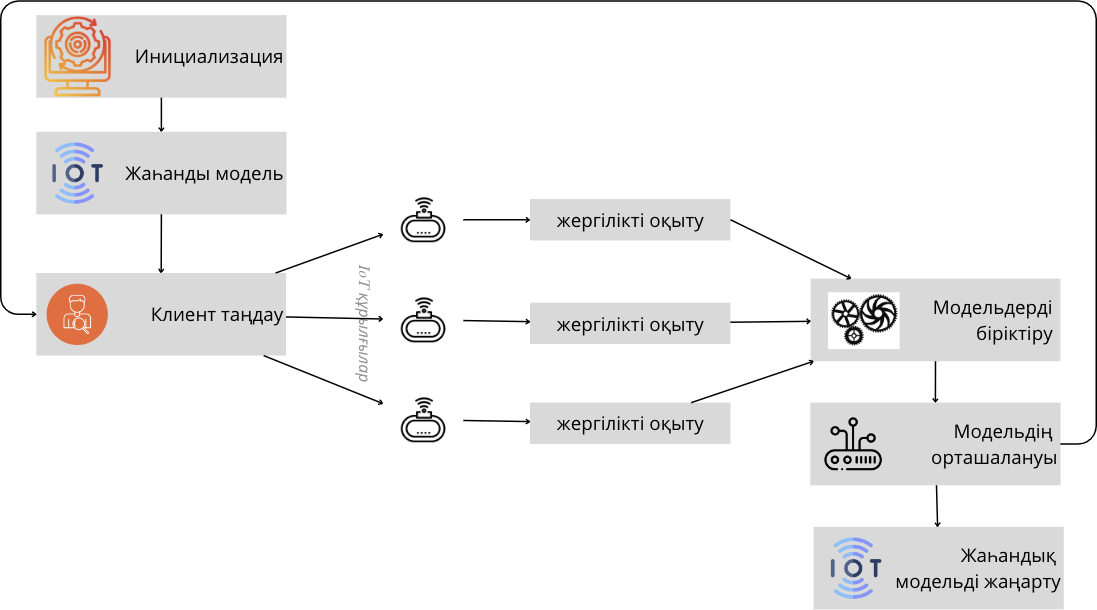
\includegraphics[width=0.8\textwidth]{assets/199}
	\caption*{}
\end{figure}

{\bfseries 1-сурет. FedAvg алгортмінің жұмыс істеу қадамдары}

Алгоритмді Google Colab ортасында Python бағдарламалау тілінде іске
асырылды, кодтың үзіндісі 2-суретте көрсетілген.

\begin{figure}[H]
	\centering
	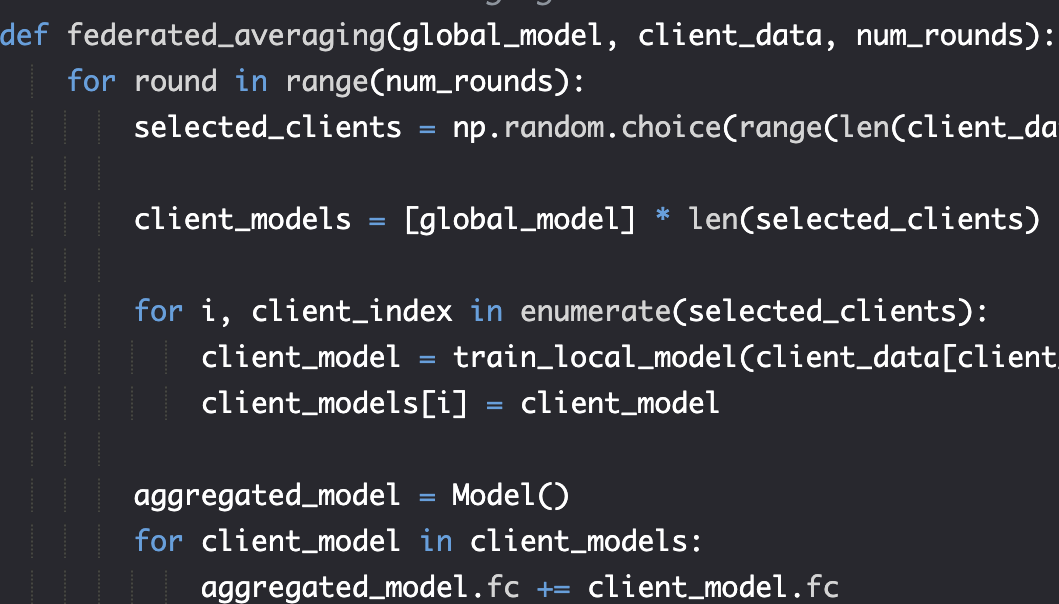
\includegraphics[width=0.8\textwidth]{assets/200}
	\caption*{}
\end{figure}

{\bfseries 2-сурет. FedAvg алгортмінің псевдокоды}

FedAvg алгортмінің псевдокодындағы \emph{federated\_averagin} функциясы
серверде федеративті орташалау үрдісін орындайды. Федеративті оқытуда
\emph{global\_model} - бастапқы модель ретінде алынып,
\emph{client\_data} әрбір клиенттен түскен деректер тізімі және
\emph{num\_rounds} раунд санын білдіреді. Әрбір таңдалған клиент өз
жергілікті моделін \emph{train\_local\_model} функциясы көмегімен
оқытады. \emph{aggregated\_model} функциясы әр клиенттік модельдің
салмақтарын қосу арқылы біріктіреді.

FedAvg - бұл IoT құрылғыларының өзра әрекеттесу барысында құпиялылық
мәселелерін шешудің және машиналық оқытудағы деректерді
орталықсыздандырудың әлеуетті әдісі {[}28{]}. FedAvg деректердің
қауіпсіздігі мен модельдің өнімділігі арасындағы мұқият тепе-теңдікті
қамтамасыз етеді, сонымен бірге пайдаланушы деректерінің құпиялылығын
сақтап, модельдерді белгілі бір құрылғыларда немесе серверлерде
жергілікті түрде оқытуға мүмкіндік береді. Ұсынылып отырған жүйенің
сұлбасы 3-суретте келтірілген.

\begin{figure}[H]
	\centering
	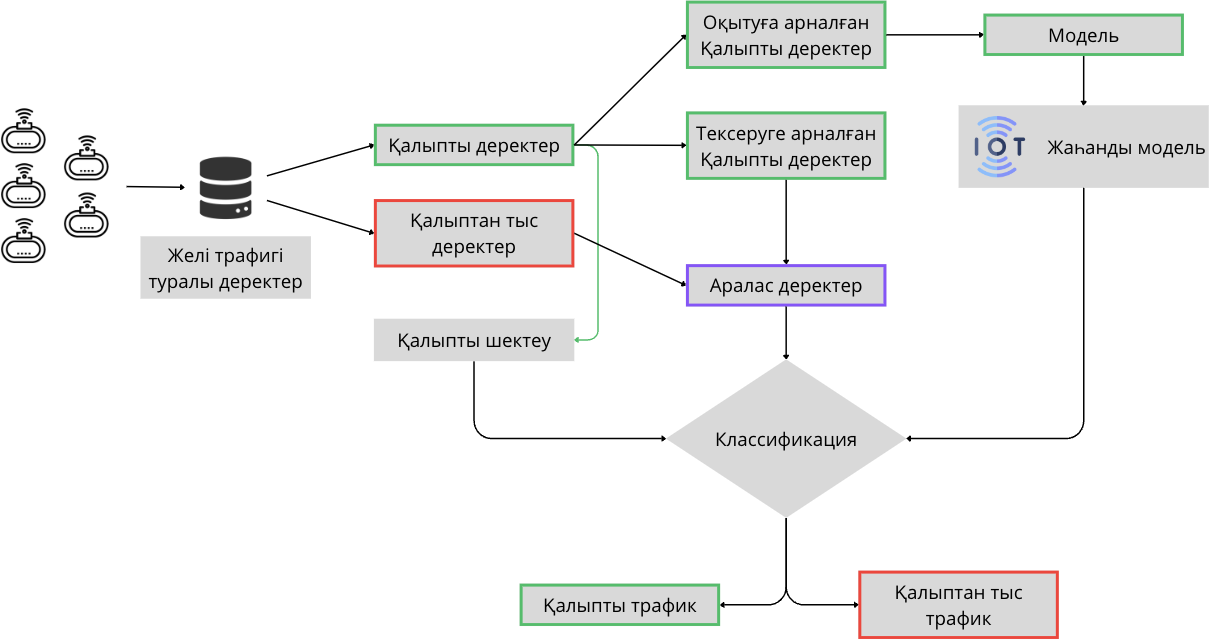
\includegraphics[width=0.8\textwidth]{assets/201}
	\caption*{}
\end{figure}

{\bfseries 3-сурет. Ұсынылған жүйе.}

Осы жұмыста ұсынылған федеративті оқыту әдісі IoT құрылғылар
желілеріндегі DDoS шабуылдар қаншалықты төмендететінін анықтау үшін
Accuracy, Precision және Recall бағалау көрсеткіштері қолданылады.
Accuracy - барлық жағдайлардың дұрыс болжанған мысалдарының пайызын
көрсете отырып, жіктеу нәтижелерінің жалпы дұрыстығын бағалайды.
Precision - модельдің жалған оң нәтижелерді азайту қабілеті туралы
түсінік бере отырып, барлық оң болжамдардың нақты оң болжамдарына үлесін
сандық түрде анықтайтын өлшем. Recall - модельдің шынайы оң жағдайларды
анықтау қабілетін көрсететін барлық нақты оң жағдайлардың шынайы оң
болжамдарының үлесін өлшейді.

{\bfseries Нәтижелер мен талқылау.} Жұмыста зерттелген федеративті оқыту
әдісі DDoS шабуылдарын анықтауда айтарлықтай тиімділік көрсетеді.
Ұсынылған әдістің бағалау өлшемдерінің көрсеткіштері 2-кесте мен
4-суретте сәйкес келтірілген. Аталған суреттерде 9 IoT құрылғы бойынша
өлшемдер көрсетілген. Нәтижесінде 4a-суретте 3 және 9 құрылғыларды
есептемегенде, алынған модельдің жоғары дәлдігі нақты көрінеді. Орта
есеппен DDOS шабуылын анықтауда алынған модельдің 99,7 \% дұрыс шешімді
болды (Сурет 4b). Модельдің шынайы оң жағдайларды анықтау қабілеті
90,0\% орта көрсеткішке жетті (Сурет 4c).

% \begin{longtable}[]{@{}
%   >{\raggedright\arraybackslash}p{(\columnwidth - 4\tabcolsep) * \real{0.3334}}
%   >{\raggedright\arraybackslash}p{(\columnwidth - 4\tabcolsep) * \real{0.3333}}
%   >{\raggedright\arraybackslash}p{(\columnwidth - 4\tabcolsep) * \real{0.3333}}@{}}
% \toprule\noalign{}
% \endhead
% \bottomrule\noalign{}
% \endlastfoot
% \begin{figure}[H]
% 	\centering
% 	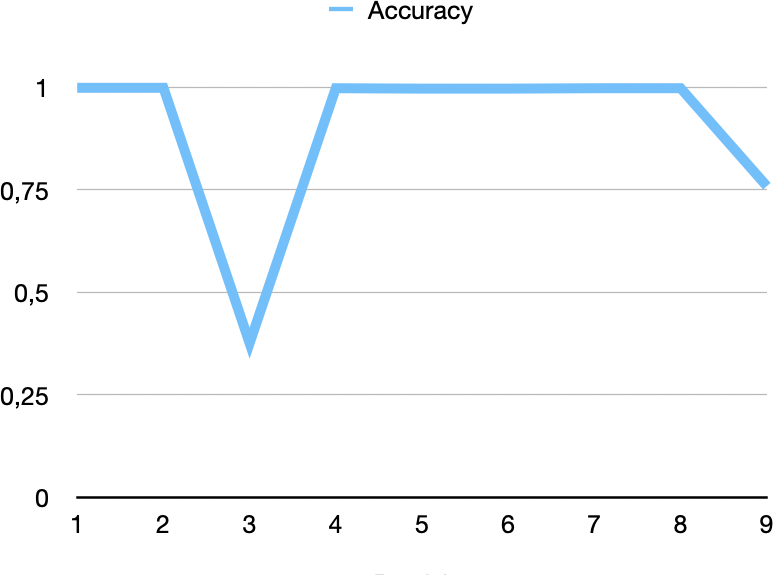
\includegraphics[width=0.8\textwidth]{assets/202}
% 	\caption*{}
% \end{figure} &
% \begin{figure}[H]
% 	\centering
% 	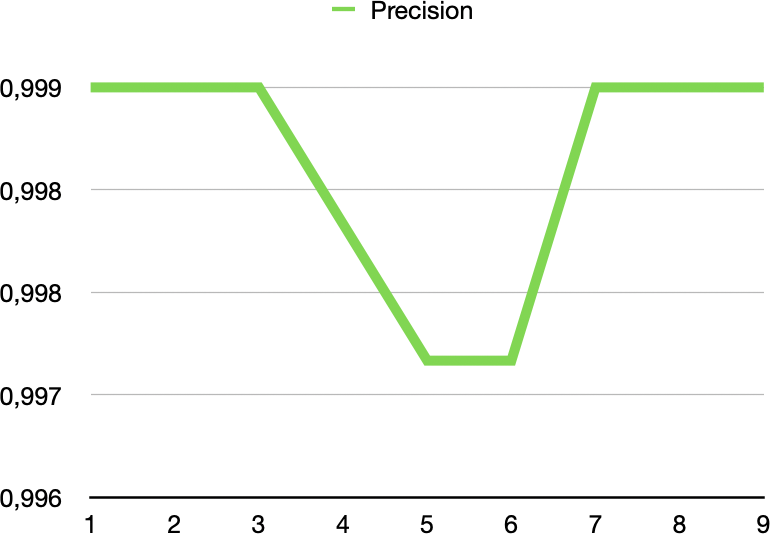
\includegraphics[width=0.8\textwidth]{assets/203}
% 	\caption*{}
% \end{figure} &
% \begin{figure}[H]
% 	\centering
% 	\includegraphics[width=0.8\textwidth]{assets/204}
% 	\caption*{}
% \end{figure} \\
% a) Accuracy & b) Precision & c) Recall \\
% \multicolumn{3}{@{}>{\raggedright\arraybackslash}p{(\columnwidth - 4\tabcolsep) * \real{1.0000} + 4\tabcolsep}@{}}{%
% {\bfseries 4-сурет. Бағалау көрсеткіштерінің құрылғыларға қатысты мәні}} \\
% \end{longtable}

Fedavg деректерді тарату теңдестірілген желілерде жақсы жұмыс істейтіні
белгілі. Алайда, деректердің таралуы әр түрлі болатын жағдайларда оның
конвергенция проблемалары бар екендігі анықталды. Бұл әдетте федералды
желілерде жиі кездесетін жағдай, мұнда әр клиент өз деректерін
пайдаланады. 2-кестеде Машиналық оқытудың түрлі әдістері көмегімен
алынған бағалау көрсеткіштерінің мәндері келтірілген. Бағалау
көрсеткіштерінің мәні көптеген факторларға тәуелді болып келеді.
Салыстырылған зерттеу жұмыстарында ашық деректер жиындары негізінде
зерттелген әдістердің қорытындысы келтірілген. Осы зерттеуде ұсынылған
жүйенің бағалау мәндері Precision бойынша жоғары көрсеткішті көрсетуде.
Бұл нәтиже федеративті оқытудың қауіпсіздік саласындағы қолданылуының
жаңа мүмкіндіктерінің болуына көз жеткізеді.

{\bfseries 2-кесте. Бағалау көрсеткіштерінің орташа мәні}

\begin{longtable}[]{@{}
  >{\raggedright\arraybackslash}p{(\columnwidth - 10\tabcolsep) * \real{0.2193}}
  >{\raggedright\arraybackslash}p{(\columnwidth - 10\tabcolsep) * \real{0.1228}}
  >{\raggedright\arraybackslash}p{(\columnwidth - 10\tabcolsep) * \real{0.1140}}
  >{\raggedright\arraybackslash}p{(\columnwidth - 10\tabcolsep) * \real{0.1380}}
  >{\raggedright\arraybackslash}p{(\columnwidth - 10\tabcolsep) * \real{0.1424}}
  >{\raggedright\arraybackslash}p{(\columnwidth - 10\tabcolsep) * \real{0.2636}}@{}}
\toprule\noalign{}
\endhead
\bottomrule\noalign{}
\endlastfoot
Өлшемдер & {[}29{]} & {[}30{]} & {[}31{]} & {[}32{]} & Ұсынылған жүйе \\
Accuracy & 94,02 & 88,76 & - & 97,7 & 90,2 \\
Precision & 88,77 & 60 & 82 & 97,1 & 99,7 \\
Recall & 89,23 & 74,36 & 71 & 97,1 & 90,0 \\
\end{longtable}

{\bfseries Қорытынды.} IoT қауіпсіздік мәселелері көп қырлы және ықтимал
кибершабуылдарды, осалдықтарды және сенімді қауіпсіздік шараларын
қабылдау қажеттілігін
қамтиды.\hspace{0pt}\hspace{0pt}\hspace{0pt}\hspace{0pt}\hspace{0pt}\hspace{0pt}\hspace{0pt}
Машиналық оқыту мен жасанды интеллектті қолдану IoT қауіпсіздігін
жақсартудың перспективалы мүмкіндіктерін ашады, ал ойластырылған
қауіпсіздік және тәуекелге негізделген қауіпсіздік механизмдері сияқты
озық тәжірибелер IoT құрылғылары мен желілерін қорғау үшін өте маңызды.
Ұсынылған жұмыста IoT құрылғыларының өзара байланыс кезінде
қауіпсіздігін арттыру мақстында федеративті оқыту әдісін қолданылу
зерттелген. Тәжірибелік зерттеу барысында 9 IoT құрылғыларының өзара
байланыс кезінде генерацияланған желілік трафик пайдаланып, жаһанды
модельді оқыту әрбір құрылғының жергілікті модельдердің көмегімен
жүргізіліп, ақпаратты жіберу барысында құпиялылықты сақтау және Ddos
шабуылдарын анықтау сұрақтарына назар аударылды. Қорытында федеративті
оқытудың қауіпсіздік деңгейін жаңа деңгейге шығару перспективасы
байқалды. бұл гипотезаны әлі де болашақ жұмыстарда зерттеу көзделуде.

IoT дәуірінде деректердің құпиялылығы барған сайын өзекті мәселеге
айналуда. Деректерді орталықтандырылған жинау және өңдеу ақпараттың ағып
кету қаупін тудырады және пайдаланушылардың құқықтарын бұзады.
Федеративті оқыту деректерді орталықтандырылған сақтаусыз талдауға
мүмкіндік беретін қауіпсіз және сенімді тәсілді ұсынады, бұл құпиялылық
тәуекелдерін айтарлықтай азайтады.

\emph{{\bfseries Қаржыландыру.} Бұл зерттеу Қазақстан Республикасы Ғылым
және жоғары білім министрлігінің Ғылым комитетімен қаржыландырған (Грант
NoAP14973006).}

{\bfseries References}

1. Karas B. (2017). Hikvision Backdoor Confirmed. IPVM
https://ipvm.com/reports/hik-backdoor

2. Porter J. (2019) Wyze server leak exposes customer data of 2.4
million users
https://www.theverge.com/2019/12/30/21042974/wyze-server-breach-cybersecurity-smart-home-security-camera

3. Cerullo M. (2024) Wyze camera breach may have let 13,000 customers
peek into others\textquotesingle{} homes
https://www.cbsnews.com/news/wyze-camera-breach-let-13000-customers-peek-into-others-homes/

4. F. Alwahedi, A. Aldhaheri, M. A. Ferrag, A. Battah, and N. Tihanyi,
Machine learning techniques for IoT security: Current research and
future vision with generative AI and large language models, Internet of
Things and Cyber-Physical Systems, vol. 4, pp. 167--185, 2024, doi:
10.1016/j.iotcps.2023.12.003.

5. M. A. Ferrag et al., ``Edge Learning for 6G-Enabled Internet of
Things: A Comprehensive Survey of Vulnerabilities, Datasets, and
Defenses,'' IEEE Communications Surveys \&amp; Tutorials, vol. 25, no.
4, pp. 2654--2713, 2023, doi: 10.1109/comst.2023.3317242.

6. R. Ahmad and I. Alsmadi, ``Machine learning approaches to IoT
security: A systematic literature review,'' Internet of Things, vol. 14,
p. 100365, Jun. 2021, doi: 10.1016/j.iot.2021.100365.

7. I. H. Sarker, A. I. Khan, Y. B. Abushark, and F. Alsolami, ``Internet
of Things (IoT) Security Intelligence: A Comprehensive Overview, Machine
Learning Solutions and Research Directions,'' Mobile Networks and
Applications, vol. 28, no. 1, pp. 296--312, Mar. 2022, doi:
10.1007/s11036-022-01937-3.

8. B. Ghimire and D. B. Rawat, ``Recent Advances on Federated Learning
for Cybersecurity and Cybersecurity for Federated Learning for Internet
of Things,'' IEEE Internet of Things Journal, vol. 9, no. 11, pp.
8229--8249, Jun. 2022, doi: 10.1109/jiot.2022.3150363.

9. L. U. Khan, W. Saad, Z. Han, E. Hossain, and C. S. Hong, ``Federated
Learning for Internet of Things: Recent Advances, Taxonomy, and Open
Challenges,'' IEEE Communications Surveys \&amp; Tutorials, vol. 23, no.
3, pp. 1759--1799, 2021, doi: 10.1109/comst.2021.3090430.

10. V. Mothukuri, P. Khare, R. M. Parizi, S. Pouriyeh, A. Dehghantanha,
and G. Srivastava, ``Federated-Learning-Based Anomaly Detection for IoT
Security Attacks,'' IEEE Internet of Things Journal, vol. 9, no. 4, pp.
2545--2554, Feb. 2022, doi: 10.1109/jiot.2021.3077803.

11. D. C. Nguyen, M. Ding, P. N. Pathirana, A. Seneviratne, J. Li, and
H. Vincent Poor, ``Federated Learning for Internet of Things: A
Comprehensive Survey,'' IEEE Communications Surveys \&amp; Tutorials,
vol. 23, no. 3, pp. 1622--1658, 2021, doi: 10.1109/comst.2021.3075439.

12. A. Imteaj, U. Thakker, S. Wang, J. Li, and M. H. Amini, ``A Survey
on Federated Learning for Resource-Constrained IoT Devices,'' IEEE
Internet of Things Journal, vol. 9, no. 1, pp. 1--24, Jan. 2022, doi:
10.1109/jiot.2021.3095077.

13. B. Breve, G. Cimino, and V. Deufemia, ``Identifying Security and
Privacy Violation Rules in Trigger-Action IoT Platforms With NLP
Models,'' IEEE Internet of Things Journal, vol. 10, no. 6, pp.
5607--5622, Mar. 2023, doi: 10.1109/jiot.2022.3222615.

14. N. Batra and S. Goyal, ``IoT architecture,'' IoT Fundamentals with a
Practical Approach, pp. 17--70, Jul. 2024, doi: 10.1201/9781003307488-2.

15. G. Sharma, S. Vidalis, N. Anand, C. Menon, and S. Kumar, ``A Survey
on Layer-Wise Security Attacks in IoT: Attacks, Countermeasures, and
Open-Issues,'' Electronics, vol. 10, no. 19, p. 2365, Sep. 2021, doi:
10.3390/electronics10192365.

16. M. Panoff, R. G. Dutta, Y. Hu, K. Yang, and Y. Jin, ``On Sensor
Security in the Era of IoT and CPS,'' SN Computer Science, vol. 2, no.
1, Jan. 2021, doi: 10.1007/s42979-020-00423-5.

17. G. M and P. H B, ``Semantic Query-Featured Ensemble Learning Model
for SQL-Injection Attack Detection in IoT-Ecosystems,'' IEEE
Transactions on Reliability, vol. 71, no. 2, pp. 1057--1074, Jun. 2022,
doi: 10.1109/tr.2021.3124331.

18. D. Javeed, M. S. Saeed, I. Ahmad, M. Adil, P. Kumar, and A. K. M. N.
Islam, ``Quantum-Empowered Federated Learning and 6G Wireless Networks
for IoT Security: Concept, Challenges and Future Directions,'' Dec.
2023, doi: 10.36227/techrxiv.170259169.96559894/v1.

19. Y. Alhasawi and S. Alghamdi, ``Federated Learning for Decentralized
DDoS Attack Detection in IoT Networks,'' IEEE Access, vol. 12, pp.
42357--42368, 2024, doi: 10.1109/access.2024.3378727

20. M. Asad, A. Moustafa, and C. Yu, ``A Critical Evaluation of Privacy
and Security Threats in Federated Learning,'' Sensors, vol. 20, no. 24,
p. 7182, Dec. 2020, doi: 10.3390/s20247182.

21. Granell, C., Kamilaris, A., Kotsev, A., Ostermann, F.O., Trilles, S.
(2020). Internet of Things. In: Guo, H., Goodchild, M.F., Annoni, A.
(eds) Manual of Digital Earth. Springer, Singapore.
https://doi.org/10.1007/978-981-32-9915-3\_11

22. Ferrag, M. A., Friha, O., Hamouda, D., Maglaras, L., \& Janicke, H.
(2022). Edge-IIoTset: A new comprehensive realistic cyber security
dataset of IoT and IIoT applications for centralized and federated
learning. IEEE Access, 10, 40281-40306.
DOI:10.36227/techrxiv.18857336.v1

23. S. Tabatabai et al., ``Exploration and Exploitation in Federated
Learning to Exclude Clients with Poisoned Data,'' 2022 International
Wireless Communications and Mobile Computing (IWCMC), May 2022, doi:
10.1109/iwcmc55113.2022.9825004.

24. V. Holubenko, P. Silva, and C. Bento, ``An Intelligent Mechanism for
Monitoring and Detecting Intrusions in IoT Devices,'' 2023 IEEE 20th
Consumer Communications \&amp; Networking Conference (CCNC), Jan. 2023,
doi: 10.1109/ccnc51644.2023.10060443.

25. K. A. Awan, I. U. Din, A. Almogren, and J. J. P. C. Rodrigues,
``Privacy-Preserving Big Data Security for IoT With Federated Learning
and Cryptography,'' IEEE Access, vol. 11, pp. 120918--120934, 2023, doi:
10.1109/access.2023.3328310.

26. M. Zang, C. Zheng, T. Koziak, N. Zilberman, and L. Dittmann,
``Federated Learning-Based In-Network Traffic Analysis on IoT Edge,''
2023 IFIP Networking Conference (IFIP Networking), Jun. 2023, doi:
10.23919/ifipnetworking57963.2023.10186438.

27. J. Mills, J. Hu, and G. Min, ``Communication-Efficient Federated
Learning for Wireless Edge Intelligence in IoT,'' IEEE Internet of
Things Journal, vol. 7, no. 7, pp. 5986--5994, Jul. 2020, doi:
10.1109/jiot.2019.2956615.

28. L. Almeida, P. Rodrigues, R. Teixeira, M. Antunes, and R. L. Aguiar,
``Privacy-Preserving Defense: Intrusion Detection in IoT using Federated
Learning,'' 2024 IEEE 22nd Mediterranean Electrotechnical Conference
(MELECON), Jun. 2024, doi: 10.1109/melecon56669.2024.10608461.

29. M. AlJamal, A. Mughaid, B. Al shboul, H. Bani-Salameh, S. Alzubi,
and L. Abualigah, ``Optimizing risk mitigation: A simulation-based model
for detecting fake IoT clients in smart city environments,'' Sustainable
Computing: Informatics and Systems, vol. 43, p. 101019, Sep. 2024, doi:
10.1016/j.suscom.2024.101019.

30. A. R. Kairaldeen, N. F. Abdullah, A. Abu-Samah, and R. Nordin,
``Peer-to-Peer User Identity Verification Time Optimization in IoT
Blockchain Network,'' Sensors, vol. 23, no. 4, p. 2106, Feb. 2023, doi:
10.3390/s23042106.

31. P. Dey, S. K. Chaulya, and S. Kumar, ``Secure decision tree twin
support vector machine training and classification process for encrypted
\textless scp\textgreater IoT\textless/scp\textgreater{} data via
blockchain platform,'' Concurrency and Computation: Practice and
Experience, vol. 33, no. 16, Mar. 2021, doi: 10.1002/cpe.6264.

32. N. Hasan, Z. Chen, C. Zhao, Y. Zhu, and C. Liu, ``IoT Botnet
Detection framework from Network Behavior based on Extreme Learning
Machine,'' IEEE INFOCOM 2022 - IEEE Conference on Computer
Communications Workshops (INFOCOM WKSHPS), May 2022, doi:
10.1109/infocomwkshps54753.2022.9798307.

\emph{{\bfseries Авторлар туралы мәліметтер}}

Адамова А. - PhD, Astana IT University, Астана, Қазақстан, e-mail:
aigul.adamova@astanait.edu.kz;

Жукабаева Т.К. - PhD, профессор, Л.Н. Гумилев атындағы Еуразия Ұлттық
университеті, Астана, Қазақстан, e-mail: tamarakokenovna@gmail.com

\emph{{\bfseries Information about the authors}}

Adamova А. - PhD, Astana IT University, Astana, Kazakhstan, e-mail:
aigul.adamova@astanait.edu.kz;

Zhukabayeva Т.К. - PhD, Professor, L. Gumilev Eurasian National
University, Astana, Kazakhstan, e-mail: tamarakokenovna@gmail.com\newpage
{\bfseries ҒТАМР 81.93.29}

{\bfseries SQL-ИНЪЕКЦИЯЛАРЫНАН ВЕБ-ҚОСЫМШАЛАР ДЕРЕКТЕР ҚОРЫНЫҢ ОСАЛДЫҒЫН
ЖӘНЕ ҚОРҒАНЫСЫН ЗЕРТТЕУ}

{\bfseries Б. Рысбекқызы\textsuperscript{🖂}, Д.Т. Кожанова, Г.К. Кабиева,
Ә.Ж. Изат, Л.Б. Кадырова,}

{\bfseries А.М. Леонтьева}

Әбілқас Сағынов атындағы Қарағанды техникалық университеті, Қарағанды,
Қазақстан

{\bfseries \textsuperscript{🖂}}Корреспондент-автор: Bakhytgulz@mail.ru

Қазіргі уақытта веб-технологиялар интернет-дүкендерде, банктерде,
кәсіпорындардың веб-парақшаларында барлық жерде қолданылады. Есесіне,
деректер қоры көбінесе веб-қосымшаларды жазу үшін қолданылады. Деректер
қоры ақпараттық қауіпсіздікке төнетін қауіптермен сипатталады.
Деректерге қол жеткізу үшін аутентификация процесінде шабуылдаушы SQL
Injection типті ақпараттық шабуылды қолдана алады. Бұл шабуылдың мәні
веб-технологиялар мен SQL қиылысындағы қатені пайдалану болып табылады.
Бұл пайдаланушы деректерін өңдеуге арналған көптеген веб-парақшалар
зиянды кодты енгізуге әкелуі мүмкін деректер қорына арнайы SQL сұранысын
қалыптастыратындығына байланысты.

Мақалада SQL инъекцияларынан веб-қосымшалар деректер қорының негізгі
қауіптері мен осалдығы қарастырылады. Жұмыс SQL инъекцияларының негізгі
түрлерін, осалдықтарды анықтау және алдын алу әдістерін және
веб-қосымшалардың осалдығын тексеру тәсілдерін талдауды қамтиды.
Деректер базасын SQL инъекцияларынан қорғау әдістеріне және тәжірибені
дамытуға баса назар аударылады.

Зерттеу тақырыбы өзекті, өйткені заманауи әлемде интернет біздің
өміріміздің ажырамас бөлігіне айналды. Қосымшаларды пайдаланудың өсуімен
құпия деректерді қорғау үшін қауіпсіздік шараларына деген қажеттілік
артты. Веб-қосымшалардың осалдығы қауіпсіздіктің бұзылуына әкелуі
мүмкін, бұл пайдаланушылардың жеке және қаржылық ақпаратын жоғалтуға,
ұйымдардың беделіне нұқсан келтіруге және заңды салдарға әкелуі мүмкін.

{\bfseries Түйін сөздер:} SQL-инъекция, веб-қосымша, деректер қоры,
деректерді қорғау, шабуыл, ақпараттық қауіпсіздік.

{\bfseries ИССЛЕДОВАНИЕ УЯЗВИМОСТИ И ЗАЩИТЫ БАЗ ДАННЫХ ВЕБ ПРИЛОЖЕНИЙ
ОТ~SQL-ИНЪЕКЦИЙ}

{\bfseries Б. Рысбекқызы\textsuperscript{🖂}, Д.Т. Кожанова Г.К. Кабиева,
А.Ж. Изат, Л.Б. Кадырова,}

{\bfseries А.М. Леонтьева}

Карагандинский технический университет имени Абылкаса Сагинова,
Караганда, Казахстан,

e-mail: Bakhytgulz@mail.ru

В настоящее время веб-технологии используются повсеместно в
интернет-магазинах, банках, веб-страницах предприятий. При этом базы
данных часто используются для написания веб-приложений. Для базы данных
характерны угрозы информационной безопасности. В процессе аутентификации
для получения доступа к данным злоумышленник может использовать
информационную атаку типа SQL Injection. Суть данной атаки заключается в
использовании ошибки на стыке веб-технологий и SQL. Это обусловлено тем,
что многие web-страницы для обработки пользовательских данных, формируют
специальный SQL запрос к базам данных, что может привести к внедрению
вредоносного кода.

В статье рассматриваются основные угрозы и уязвимость баз данных
веб-приложений от SQL-инъекций. Работа включает в себя анализ основных
видов SQL-инъекций, методов обнаружения и предотвращения уязвимостей, а
также подходы к тестированию уязвимостей веб-приложений. Основное
внимание уделено методам защиты баз данных от SQL-инъекций и разработке
практических рекомендаций по обеспечению безопасности веб-приложений.

Тематика исследования актуальна так как в современном мире, так как
интернет стал неотъемлемой частью нашей жизни. С ростом использования
приложений также возросла потребность в мерах безопасности для защиты
конфиденциальных данных. Уязвимости веб-приложений могут привести к
нарушениям безопасности, что может привести к потере личной и финансовой
информации пользователей, ущербу для репутации организаций и юридическим
последствиям.

{\bfseries Ключевые слова:} SQL-инъекция; веб-приложение; базы данных;
защита данных; атака; информационная безопасность.

{\bfseries RESEARCH OF VULNERABILITY AND PROTECTION OF WEB APPLICATION
DATABASES FROM SQL INJECTIONS}

{\bfseries B. Rysbekyzy\textsuperscript{🖂}, D.T. Kozhanova G.K. Kabieva,
A.Zh. Izat, L.B.Kadyrova,}

{\bfseries A.M.Leontyeva}

Abylkas Saginov Karaganda Technical University, Karaganda, Kazakhstan,

e-mail: Bakhytgulz@mail.ru

Currently, web technologies are used everywhere in online stores, banks,
and enterprise web pages. At the same time, databases are often used to
write web applications. The database is characterized by information
security threats. During the authentication process, an attacker can use
an information attack such as SQL Injection to gain access to data. The
essence of this attack is to exploit an error at the intersection of web
technologies and SQL. This is due to the fact that many web pages form a
special SQL query to databases to process user data, which can lead to
the introduction of malicious code.

The article discusses the main threats and vulnerability of web
application databases from SQL injections. The work includes an analysis
of the main types of SQL injections, methods for detecting and
preventing vulnerabilities, as well as approaches to testing web
application vulnerabilities. The main focus is on methods for protecting
databases from SQL injections and developing practical recommendations
for ensuring the security of web applications.

The topic of the research is relevant in the modern world, since the
Internet has become an integral part of our lives. As the use of apps
has increased, the need for security measures to protect sensitive data
has also increased. Web application vulnerabilities can lead to security
breaches that can result in the loss of users\textquotesingle{} personal
and financial information, damage to organizations\textquotesingle{}
reputations, and legal consequences.

{\bfseries Key words:} SQL injection; web application; databases; data
protection; attack; information security.

{\bfseries Кіріспе.} Веб-қосымшадағы шабуылдардың ең танымал түрлерінің
бірі SQL инъекциясы болып табылады. SQL-инъекция - бұл зиянды
пайдаланушыға өзінің жеке параметрлерін қолданыстағы SQL-сұраныс
жасауына немесе SQL-сұраныс жасауды болдырмауға және өзінің жеке сұраныс
жасауын ұсынуға мүмкіндік беретін SQL дерекқорына арнайы бағытталған
инъекциялық шабуыл түрі.

SQL-инъекция ең кең таралған, бірақ жалғыз түрі емес. Инъекциялық
шабуылдар екі негізгі компоненттен тұрады: интерпретатор және
пайдаланушыдан түсетін пайдалы жүктеме, ол қандай да бір интерпретаторға
оқылады {[}1-2{]}. Бұл инъекциялық шабуылдар FFMPEG (бейнекомпрессор)
сияқты командалық жолдың утилитасына, сондай-ақ, деректер қорына
(дәстүрлі жағдайда SQL-инъекцияға) қарсы болуы мүмкін дегенді білдіреді.

{\bfseries Материалдар мен әдістер.} SQL-инъекция ең классикалық аталатын
инъекция түрі болып табылады. SQL жолы HTTP пайдалы жүктемесінде
экрандалады, бұл соңғы пайдаланушының атынан пайдаланушы SQL
сұраныстарына әкеледі.

Дәстүрлі түрде көптеген OSS пакеттері PHP және SQL (жиі MySQL)
комбинациясын пайдалана отырып жасалған. Әзірлеу тарихындағы
SQL-инъекциялардың көптеген жиі айтылған осалдықтары PHP-нің түсініктер,
логика және деректер коды арасындағы интерполяцияға неғұрлым жұмсақ
тәсілді ұстануы нәтижесінде туындады. Ескі мектептің PHP әзірлеушілері
өздерінің PHP файлдарында SQL, HTML және PHP комбинацияларын - PHP
қолдайтын ұйымдастыру моделін қолданар еді, ол дұрыс қолданылмай, бұл
осал PHP кодының көп болуына әкелетін еді.

Пайдаланушыға жүйеге кіруге мүмкіндік беретін форумның ескі
бағдарламалық жасақтамасына арналған PHP код блогының мысалын
қарастырайық:

\textless?php {\bfseries if}
(\$\_SERVER{[}\textquotesingle REQUEST\_METHOD\textquotesingle{]} !=
\textquotesingle POST\textquotesingle) \{

{\bfseries echo}\textquotesingle{}

\textless div class="row"\textgreater{}

\textless div class="small-12 columns"\textgreater{}

\textless form method="post" action=""\textgreater{}

\textless fieldset class="panel"\textgreater{}

\textless center\textgreater{}

\textless h1\textgreater Sign
In\textless/h1\textgreater\textless br\textgreater{}

\textless/center\textgreater{}

\textless label\textgreater{}

\textless Input type="text" id="username" name="username"
placeholder="Username"\textgreater{}

\textless/label\textgreater{}

\textless label\textgreater{}

\textless input type="password" id="password" name="password"
placeholder="Password"\textgreater{}

\textless/label\textgreater{}

\textless center\textgreater{}

\textless input type="submit" class="button" value="Sign
In"\textgreater{}

\textless/center\textgreater{}

\textless/fieldset\textgreater{}

\textless/form\textgreater{}

\textless/div\textgreater{}

\textless/div\textgreater\textquotesingle;

\} {\bfseries else} \{

// the user has already filled out the login form.

// pull in database info from config.php

\$Servername = getenv(\textquotesingle IP\textquotesingle);

\$Username = \$mysqlUsername;

\$Password = \$mysqlPassword;

\$Database = \$mysqlDB;

\$Dbport = \$mysqlPort;

\$database = {\bfseries new} mysqli(\$servername, \$username, \$password,
\$database,\$dbport);

{\bfseries if} (\$database-\textgreater connect\_error) \{

{\bfseries echo} "ERROR: Failed to connect to MySQL";

{\bfseries die};

\}

\$sql = "SELECT userId, username, admin, moderator FROM users WHERE
username =
\textquotesingle".\$\_POST{[}\textquotesingle username\textquotesingle{]}."\textquotesingle{}
AND password =
\textquotesingle".sha1(\$\_POST{[}\textquotesingle password\textquotesingle{]})."\textquotesingle;";

\$result = mysqli\_query(\$database, \$sql);

\}

Көріп отырғаныңыздай, берілген кіру кодында PHP, SQL және HTML
араласқан. Сонымен қатар, SQL-сұранысы сұраныс жолағын жасамас бұрын
ешқандай тазартусыз сұрау параметрлерін біріктіру негізінде жасалады
{[}3{]}.

HTML, PHP және SQL кодтарының тоғысуы PHP негізіндегі веб-қосымшалар
үшін SQL инъекциясының енуіне едәуір жеңілдетті. Тіпті WordPress сияқты
кейбір ірі OSS PHP қосымшалары бұған дейін осындай жағдайдың құрбаны
болған.

PHP-ден алынған қауіпсіздік сабақтары басқа тілдерде көрініс тапты және
қазіргі заманғы веб-қосымшаларда SQL-ді енгізуге байланысты осалдықтарды
табу әлдеқайда қиын. Дегенмен, бұл әлі де мүмкін және қауіпсіз
бағдарламалаудың озық әдістерін қолданбайтын қосымшаларда жиі кездеседі.

{\bfseries Нәтижелер мен талқылау. \emph{Инъекцияға қарсы қорғаныстарды
зерттеу.}} Әдетте әзірлеушінің CLI және пайдаланушы жіберген деректері
бар автоматтандырудың кез келген түрін жазуына дұрыс назар аудармауының
нәтижесінде бұл шабуылдар әлі де жиі кездеседі.

Инъекциялық шабуылдар сондай-ақ, жазықтықтың кең ауданын қамтиды.
Инъекцияны CLI-ге немесе серверде жұмыс істейтін кез келген басқа
оқшауланған интерпретаторға қарсы пайдалануға болады (ол ОЖ деңгейіне
жеткенде, оның орнына ол команда инъекциясына айналады) {[}4-5{]}.
Нәтижесінде, инъекция стиліндегі шабуылдардан қалай қорғанатынымызды
қарастырғанда, мұндай қорғау шараларын бірнеше санатқа бөлу оңай.

Ең алдымен, біз SQL-инъекция шабуылдарынан қорғанысты бағалауымыз керек
- инъекцияның ең кең тараған және белгілі түрі. SQL инъекцияларынан
қорғану үшін не істей алатынымызды зерттегеннен кейін, бұл
қорғаныстардың қайсысы инъекциялық шабуылдардың басқа түрлеріне
қолданылатынын көруге болады. Ақыр соңында, біз инъекциядан қорғаудың
бірнеше жалпы әдістерін бағалай аламыз, олар инъекцияның негізіндегі
шабуылдардың қандай да бір жиынына тән емес.

\emph{SSQL-инъекциясының салдарын жұмсарту{\bfseries . }}SQL инъекциясы --
инъекциялық шабуылдың ең көп таралған түрі және сол сияқты қорғанудың ең
оңай түрлерінің бірі. Ол өте кең таралғандықтан, әрбір дерлік күрделі
веб-қосымшаға әсер етуі мүмкін (SQL дерекқорларының таралуына
байланысты) SQL инъекциясына қарсы көптеген жұмсарту және қарсы шаралар
әзірленді.

Сонымен қатар, SQL инъекциялық шабуылдар SQL интерпретаторында орын
алатындықтан, мұндай осалдықтарды анықтау өте қарапайым болуы мүмкін
{[}6{]}. Тиісті анықтау және жұмсарту стратегиялары бар болса,
веб-қосымшаның SQL инъекциялық шабуылына ұшырау мүмкіндігі өте төмен.

\emph{SQL инъекциясын анықтау.} Кодтық базаңызды SQL инъекциялық
шабуылдардан қорғауға дайындау үшін алдымен SQL инъекциясы қабылдайтын
форманы және сіздің кодтық базаңыздағы ең осал болуы мүмкін орындарды
қарап шығуыңыз керек {[}7{]}.

Көптеген заманауи веб-қосымшаларда SQL операциялары сервер жағындағы
маршрутизация деңгейінен кейін орындалады. Бұл клиент туралы ештеңе
қызықтырмайтынын білдіреді.

Мысалы, веб-қосымшаның код репозиторийінің файлдық құрылымы бар, ол
келесідей:

/api

/routes

/utils

/analytics

/routes

/client

/pages

/scripts

/media

Біз клиентті іздеуді жіберіп алатынымызды білеміз, бірақ біз талдау
бағытын қарастыруымыз керек, өйткені ол OSS-те салынған болса да, ол
аналитика деректерін сақтау үшін қандай да бір дерекқорды пайдалануы
мүмкін. Егер деректер құрылғылар мен сессиялар арасында сақталса, олар
серверлік жадта, дискіде (журналдарда) немесе дерекқорда сақталады.

Серверде көптеген қолданбалар бірден көп дерекқорды пайдаланатынын
білуіміз керек. Бұл қолданба, мысалы, SQL Server-ді және MySQL-ді
пайдаланады дегенді білдіруі мүмкін. Сондықтан сервердегі іздеу кезінде
SQL сұраныстарын бірнеше SQL тілінің іске асырылуынан табу үшін ортақ
сұраныстарды пайдалану қажет.

Бұдан басқа, кейбір серверлік бағдарламалар доменге тән тілді (DSL)
пайдаланады, ол біздің атымыздан SQL шақыруларын орындауы мүмкін, бірақ
бұл шақырулар өңделмеген SQL шақыруына ұқсас құрылымданбайды.

Қолданыстағы кодтық базаны SQL-инъекцияның әлеуетті тәуекелдеріне дұрыс
талдау жасау үшін, біз барлық алдыңғы DSL және SQL түрлерінің тізімін
жасап, оны бір жерде сақтауымыз керек.

Егер біздің қолданба Node.js қолданбасы болып табылса және ол мыналарды
қамтыса:

\begin{itemize}
\item
  SQL сервері -- NodeMSSQL адаптері (npm) арқылы
\item
  MySQL -- mysql адаптері (npm) арқылы
\end{itemize}

онда екі SQL іске асыруынан SQL сұраныстарын таба алатын код базасында
іздеулерді құрылымдауды қарастыруымыз керек.

Бақытымызға орай, Node.js-пен жеткізілетін модульдерді импорттау жүйесі
бұл тапсырманы JavaScript тілінің қолданылу аймағымен бірге жеңілдетеді
{[}8{]}. Егер SQL кітапханасы пермодуль негізінде импортталса,
сұрауларды табу импортты іздеу сияқты оңай болады:

const sql = require(\textquotesingle mssql\textquotesingle)

// OR

const mysql = require(\textquotesingle mysql\textquotesingle);

Екінші жағынан, егер бұл кітапханалар жаһандық деңгейде жарияланса
немесе ата-аналық класстан мұраға қалса, іздеу жұмыстары біршама
күрделене түседі.

Node.js үшін жоғарыда аталған екі SQL адаптерінің екеуі де .query (x)
шақыруымен аяқталатын синтаксисті қолданады, бірақ кейбір адаптерлер
әріптік синтаксисті қолданады:

const sql = require(\textquotesingle sql\textquotesingle);

const getUserByUsername = function(username) \{

const q = new sql();

q.select(\textquotesingle*\textquotesingle);

q.from(\textquotesingle users\textquotesingle);

q.where(`username = \$\{username\}`);

q.then((res) =\textgreater{} \{

return `username is : \$\{res\}`;

\});

\};

\emph{Дайындалған нұсқаулықтар.} Жоғарыда айтылғандай, SQL-сұраныстар
бұрын кең таралған және өте қауіпті. Бірақ көптеген жағдайларда олардан
қорғану онша қиын емес.

SQL-ді іске асырудың көпшілігі қолдай бастаған әзірлемелердің бірі
дайындалған операторлар болып табылады. Дайындалған нұсқаулықтар
SQL-сұраныстарда пайдаланушылар ұсынатын деректерді пайдалану кезінде
тәуекелді едәуір төмендетеді. Сонымен қатар, дайындалған нұсқаулықтар
өте оңай зерттеледі және SQL-сұраныстарды түзетуді айтарлықтай
жеңілдетеді {[}9{]}.

Дайындалған нұсқаулықтар көбінесе инъекциядан қорғаудың «бірінші желісі»
болып саналады. Дайындалған нұсқаулықтарды іске асыру оңай, Интернетте
жақсы құжатталған және инъекциялық шабуылдарды тоқтату үшін өте тиімді.

Дайындалған нұсқаулықтар айнымалылар үшін толтырғыш мәндері бар
сұранысты алдын ала құрастыру арқылы жұмыс істейді. Олар байланыстырушы
айнымалылар ретінде белгілі, бірақ көбінесе жай толтырғыш айнымалылар
деп аталады. Сұраныс құрастырылғаннан кейін толтырғыштар әзірлеуші
ұсынған мәндермен ауыстырылады. Осы екі сатылы процестің нәтижесінде
сұраныс мақсаты пайдаланушы жіберген кез келген деректер қаралмай тұрып
белгіленеді.

Дәстүрлі SQL сұрауында пайдаланушы жіберген деректер (айнымалылар) және
сұраныстың өзі дерекқорға жол ретінде бірге жіберіледі. Бұл дегеніміз,
егер пайдаланушы деректері манипуляцияланса, бұл сұраныстың ниетін
өзгерте алады.

Дайындалған нұсқаулықты пайдаланған кезде, сұраныстың мақсаты
пайдаланушы жіберген деректер SQL интерпретаторына жіберілмес бұрын
нақты анықталғандықтан, сұраныстың өзін өзгерту мүмкін емес. Бұл
пайдаланушыларға арналған SELECT операциясын кез келген жолмен
экрандауға және ЖОЮ операциясына түрлендіруге болмайтынын білдіреді.
Егер пайдаланушы бастапқы сұранысты орындамаса және жаңасын бастаса,
SELECT операциясынан кейін қосымша сұранысты орындау мүмкін емес.
Дайындалған нұсқаулар SQL енгізу тәуекелдерінің көпшілігін жояды және
барлық дерлік негізгі SQL дерекқорларымен қамтамасыз етіледі: MySQL,
Oracle, PostgreSQL, Microsoft SQL Server және т.б.

Дәстүрлі SQL-сұраныстар мен дайындалған нұсқаулықтар арасындағы жалғыз
маңызды ымыраласу өнімділік болып табылады {[}10-11{]}. Дерекқорға бір
өтініштің орнына дерекқор дайындалған нұсқаулықты ұсынады, одан кейін
компиляциядан кейін және сұранысты орындау кезінде енгізу үшін
айнымалылар болады. Көптеген қосымшаларда бұл өнімділікті жоғалту
минималды болады.

Синтаксистік тұрғыдан дайындалған нұсқаулықтар дерекқордан дерекқорға
және адаптерден адаптерге ерекшеленеді.

MySQL-де дайындалған нұсқаулықтар өте қарапайым келеді:

PREPARE q FROM \textquotesingle SELECT name, barCode from products WHERE
price \textless= ?\textquotesingle;

SET @price = 12;

EXECUTE q USING @price;

DEALLOCATE PREPARE q;

Осы дайындалған нұсқаулықта біз бағасы төмен өнімдер үшін MySQL
дерекқорынан сұраймыз (біз аты мен штрих кодын қайтарғымыз келеді)?.

Біріншіден, сұранысымызды q атауымен сақтау үшін PREPARE операторын
қолданамыз. Бұл сұраныс құрылады және пайдалануға дайын болады. Әрі
қарай, @price айнымалы мәнін 12 мәніне меншіктейміз. Бұл, мысалы,
электрондық коммерция сайтына қарсы сүзгіден өткізетін пайдаланушылар
орнатуы үшін жақсы айнымалы болар еді. Содан кейін біз ? толтыру үшін
@price беретін сұрауды орындаймыз. Соңында, біз оны жадтан жою үшін q
бойынша DEALLOCATE қолданамыз, осылайша оның атаулар кеңістігі басқа
нәрселер үшін пайдаланылуы мүмкін.

Бұл қарапайым дайындалған нұсқаулықта q @price көмегімен орындалмас
бұрын құрастырылады. Егер @price 5-ке тең болса да; UPDATE users WHERE
id = 123 SET balance =10000, қосымша сұрау деректермен
құрастырылмағандықтан іске қосылмайды.

Бұл сұраудың әлдеқайда қауіпсіз нұсқасы:

\textquotesingle SELECT name, barcode from products WHERE price
\textless= \textquotesingle{} + price +
\textquotesingle;\textquotesingle{}

Сіз анық көріп отырғаныңыздай, дайындалған нұсқаулықтарды алдын ала
құрастыру SQL инъекцияларын жеңілдетудегі маңызды бірінші қадам болып
табылады және оны веб-қосымшаңызда мүмкін болған жерде пайдалану керек
{[}12{]}.

\emph{Деректер қорына тән қорғаныстар.} Кеңінен қабылданған дайындалған
нұсқаулықтарға қосымша әрбір SQL негізгі дерекқоры қауіпсіздікті арттыру
үшін өзінің жеке функцияларын ұсынады. Oracle, MySQL, MS SQL және SOQL
SQL сұраныстарында пайдалану үшін қауіпті деп саналатын таңбалар мен
таңбалар жиынтығын автоматты түрде экрандау әдістерін ұсынады. Осы
санациялар туралы шешім қабылданатын әдіс нақты пайдаланылатын дерекқор
мен механизмге байланысты болады.

Oracle (Java) келесі синтаксиспен шақырылуы мүмкін кодтаушыны ұсынады:

ESAPI.encoder().enodeForSQL(new OracleCodec(), str);

Осыған ұқсас, MySQL баламалы функционалдылықты ұсынады. MySQL
бағдарламасында дұрыс экрандалмаған жолдарды пайдалануды болдырмау үшін
мыналарды пайдалануға болады:

SELECT
QUOTE(\textquotesingle test\textquotesingle\textquotesingle case\textquotesingle);

MySQL жүйесіндегі QUOTE функциясы кері қиғаш сызықтарды, жалғыз
тырнақшаларды немесе NULL мәндерін болдырмайды және бір тырнақшалы жолды
дұрыс қайтарады.

MySQL mysql\_real\_escape\_string () ұсынады. Бұл функция барлық алдыңғы
қисық сызықтарды және жалғыз тырнақшаларды болдырмайды, сонымен қатар,
қос тырнақшаларды ,\textbackslash n және\textbackslash r (linebreak)
болдырмайды.

Қатерлі таңбалар жиынтығын айналып өту үшін дерекқорға тәуелді жолдарды
тазалау құралдарын пайдалану жолдан айырмашылығы SQL-литералды жазуды
қиындата отырып, SQL-инъекция тәуекелін төмендетеді. Егер параметрленуі
мүмкін емес сұраныс орындалса, олар әрқашан пайдаланылуы тиіс - бірақ
оларды жан-жақты қорғау ретінде емес, жұмсарту ретінде қарау керек.

\emph{Жалпы инъекциялық қорғаныс.} SQL инъекцияларынан қорғану
мүмкіндігіне қоса, сіз сондай-ақ, сіздің қосымшаңыздың инъекцияның басқа
аз таралған түрлерінен қорғалғанына көз жеткізуіңіз керек {[}13{]}.
Жоғарыда айтылғандай, инъекциялық шабуылдар командалық жолдың немесе
интерпретатордың утилитасының кез келген түріне қарсы болуы мүмкін.

Біз SQL инъекцияларынан басқа мақсаттарды іздеуге және инъекцияға
күтпеген осалдықтың пайда болу қаупін азайту үшін барлық қолданбаның
логикасында әдепкі кодтау әдістерін қолдануға тиіспіз.

\emph{Инъекцияларға арналған ықтимал мақсаттар.} Біз бейне немесе
суреттерді сығудың CLI интерфейстері әлеуетті енгізу мақсаты ретінде
пайдаланылуы мүмкін сценарийді қарастырған болатынбыз. Бірақ енгізу
FFMPEG сияқты командалық жолдың утилиттерімен шектелмейді. Ол мәтіндік
енгізуді қабылдайтын және мәтінді қандай да бір интерпретатордың
көмегімен түсіндіретін немесе мәтінді қандай да бір командалар тізімімен
салыстыратын скрипттің кез келген түріне қолданылады.

Әдетте, жүйеге енгізуді іздеу кезінде тәуекел дәрежесі жоғары мынадай
объектілер пайдаланылады:

- Міндеттерді жоспарлаушылар

- Қысу/оңтайландыру кітапханалары

- Қашықтағы сақтық көшірме скрипттері

- Дерекқорлар

- Тіркеушілер

- Хосттың кез келген операциялық жүйесін шақыру

- Кез келген интерпретатор немесе компилятор

Сіздің веб-қосымшаңыздың компоненттерін енгізудің әлеуетті тәуекелі
тұрғысынан бірінші рет ранжирлеу кезінде оларды жоғарыда келтірілген
жоғары тәуекел объектілерінің тізімімен салыстырыңыз. Бұл сіздің
зерттеуіңізге арналған бастапқы нүктелеріңіз болып табылады.

Тәуелділіктер де тәуекел болуы мүмкін, себебі көптеген тәуелділіктер
өздерінің (суб) тәуелділіктерін әкеледі, олар көбінесе осы санаттардың
біріне түсуі мүмкін.

\emph{Ең аз өкілеттілік принципі. Ең аз өкілеттілік принципі} (көбінесе
ең аз артықшылықтар принципі деп аталады) абстракцияның маңызды ережесі
болып табылады, оны қауіпсіз веб-қосымшаларды құруға тырысу кезінде
әрқашан пайдалану керек. Бұл принцип кез келген жүйеде жүйенің әрбір
мүшесінің өз жұмысын орындау үшін қажетті ақпарат пен ресурстарға ғана
қол жеткізуі керек екенін айтады.

Бағдарламалық қамтамасыз ету әлемiнде мынадай принцип қолданылуы мүмкiн:
«бағдарламалық жүйедегi әрбiр модуль осы модульдiң дұрыс жұмыс iстеуi
үшiн қажеттi деректер мен функцияларға ғана қол жеткiзуге тиiс».

Теорияда бұл қарапайым болып көрінеді, бірақ қажет болған жағдайда
масштабты веб-қосымшаларда сирек қолданылады. Бұл принцип шын мәнінде
маңыздырақ болады, өйткені қолданба күрделілігі бойынша масштабталады,
өйткені күрделі қолданбадағы модульдер арасындағы өзара әрекеттесу
күтпеген жанама әсерлер әкелуі мүмкін.

Веб-қосымшаңызбен біріктірілген және пайдаланушы профильдерінің
фотосуреттерінің сақтық көшірмесін автоматты түрде жасайтын пәрмен жолы
интерфейсін жасап жатқаныңызды елестетіп көріңіз {[}14{]}. Бұл CLI
терминалдан (қолмен сақтық көшірме жасау) немесе веб-қосымшаңыз
орнатылған бағдарламалау тілінде жазылған адаптер арқылы шақырылады.
Егер бұл CLI ең аз өкілеттік қағидаты бойынша құрылған болса, онда CLI
бұзылған болса да, қосымшаның қалған бөлігі бұзылмас еді. Екінші
жағынан, әкімші ретінде орындалатын CLI алаяқтық инъекциялық шабуыл
анықталған және жұмыс істеген жағдайда бүкіл қолданба серверін аша
алады.

Ең аз өкілеттілік принципі әзірлеушілер үшін кедергі болып көрінуі
мүмкін - қосымша жазбаларды, бірнеше кілттерді басқару және т.б. - бірақ
осы қағидатты дұрыс іске асыру сіздің қосымшаңыз бұзылған жағдайда
ұшырайтын тәуекелді шектейді.

\emph{Ақ тізімге қосу пәрмендері.} Инъекция үшін ең үлкен қауіп - бұл
клиент (пайдаланушы) орындау үшін серверге командалар жіберетін
веб-қосымшадағы функционалдылық. Бұл нашар архитектуралық тәжірибе және
оны кез келген жағдайда болдырмау керек {[}15{]}.

Пайдаланушы таңдаған пәрмендер серверде кез келген контексте орындалуы
керек болғанда, оларға әлеуетті нұқсан келтіруге немесе қолданбаның
күйін өзгертуге (дұрыс пайдаланбаған жағдайда) мүмкіндік беретін қосымша
қадамдар қажет болады. Пайдаланушы пәрмендерінің сервермен тікелей
түсіндірілуіне мүмкіндік берудің орнына, пайдаланушыға қолжетімді
пәрмендердің нақты анықталған ақ тізімін жасау керек. Бұл команда
синтаксисіне (тәртібі, жиілігі, параметрлері) қосымша ретінде барлығын
қара тізім форматында емес, ақ тізім форматында сақтай отырып, бірге
пайдаланылуы тиіс. Келесі мысалды қарастырайық:

Келесі мысалды қарастырайық:

\textless div class="options"\textgreater{}

\textless h2\textgreater Commands\textless/h2\textgreater{}

\textless input type="text" id="command-list"/\textgreater{}

\textless button type="button"
onclick="sendCommands()"\textgreater Серверге пәрмендерді жіберу
\textless/button\textgreater{}

\textless/div\textgreater{}

const cli = require(\textquotesingle../util/cli\textquotesingle);

/*

* Клиенттен пәрмендерді қабылдайды, оларды CLI-ге қарсы іске қосады.

*/

const postCommands = function(req, res) \{

cli.run(req.body.commands);

\};

Бұл жағдайда клиент CLI кітапханасы қолдайтын кез-келген командаларды
серверге қарсы орындай алады. Бұл дегеніміз, CLI жұмыс уақыты мен толық
көлемі Соңғы пайдаланушыға CLI қолдайтын командаларды беру арқылы қол
жетімді, тіпті егер олар әзірлеуші қолдануға арналмаған болса да.

Неғұрлым түсініксіз жағдайда, барлық пәрмендерге әзірлеуші рұқсат берген
болуы мүмкін, бірақ синтаксис, тәртіп және жиілік серверде CLI-ге қарсы
күтпеген функционалдық (инъекция) жасау үшін біріктірілуі мүмкін. Тез
және лас жұмсарту - бұл тек бірнеше командалардың ақ тізімі:

{\bfseries const} cli =
require(\textquotesingle../util/cli\textquotesingle);

{\bfseries const} commands = {[}

\textquotesingle print\textquotesingle,

\textquotesingle cut\textquotesingle,

\textquotesingle copy\textquotesingle,

\textquotesingle paste\textquotesingle,

\textquotesingle refresh\textquotesingle{}

{]};

\emph{/*}

/*

* Клиенттен пәрмендерді қабылдайды, егер олар ақ тізім массивінде пайда
болса,

* оларды ТЕК CLI-ге қарсы іске қосады.

*/

{\bfseries const} postCommands = {\bfseries function}(req, res) \{

{\bfseries const} userCommands = req.body.commands;

userCommands.forEach((c) =\textgreater{} \{

{\bfseries if} (!commands.includes(c)) \{ {\bfseries return}
res.sendStatus(400); \}

\});

cli.run(req.body.commands);

\};

Бұл жылдам және лас жұмсарту командалардың ретіне немесе жиілігіне
қатысты мәселелерді шеше алмауы мүмкін, бірақ бұл клиент немесе соңғы
пайдаланушы пайдалануға арналмаған командаларды шақыруға жол бермейді
{[}16{]}. Қара тізім қолданылмайды, өйткені қосымшалар уақыт өте келе
дамиды. Қара тізімдер пайдаланушыға қажетсіз функционалдылық деңгейлерін
беретін жаңа пәрмен қосылған жағдайда қауіпсіздік қаупі ретінде
қарастырылады.

Пайдаланушы енгізуі қабылданып, CLI-ге жіберілген кезде, әрқашан қара
тізім тәсілін емес, ақ тізім тәсілін таңдаңыз.

{\bfseries Қорытынды.} Инъекциялық шабуылдар классикалық түрде деректер
қорына, атап айтқанда SQL деректер қорына жатады. Бірақ дерекқорлар
дұрыс жазылған кодсыз және конфигурациясыз инъекциялық шабуылдарға осал
болса да, API соңғы нүктесі (немесе тәуелділік) өзара әрекеттесетін кез
келген CLI инъекцияның құрбаны болуы мүмкін.

Негізгі SQL дерекқорлары SQL инъекциясының алдын алу шараларын ұсынады,
бірақ SQL инъекциясы қолданбаның архитектурасымен және қате жазылған
клиент-сервер кодымен әлі де мүмкін. Кодтық базаға ең аз өкілеттік
принципін енгізу сіздің ұйымыңызға және веб-қосымшаңыздың
инфрақұрылымына келтірілген зиянды азайту арқылы бұзылған жағдайда
веб-қосымшаңызға көмектеседі. Бастапқыда қауіпсіздік принциптеріне
негізделген қосымша ешқашан клиентке (пайдаланушыға) серверде
орындалатын сұраныс немесе пәрмен беруге мүмкіндік бермейді.

Егер пайдаланушы енгізген деректерді сервер жағындағы операцияларға
түрлендіру қажет болса, бұл операциялар жалпы функционалдылықтың бір
бөлігі ғана қолжетімді болуы үшін және қауіпсіздікті тексерудің жауапты
тобы қауіпсіз ретінде тексерген функционалдылық қана ақ тізімге
енгізілуі тиіс.

Осы басқару элементтерін пайдалана отырып, веб-қосымша инъекция
стиліндегі осалдыққа ие болу ықтималдығы әлдеқайда төмен болады.

SQL-инъекция шабуылдары кеңінен танымал және оларға дайын болғанымен,
инъекция шабуылдары сервер API сұранысына жауап ретінде пайдаланатын кез
келген CLI утилитасына қарсы болуы мүмкін.

SQL дерекқоры (жиі) инъекциядан жақсы қорғалған. Автоматтандыру белгілі
SQL-инъекция шабуылдарын тестілеу үшін өте ыңғайлы, өйткені шабуыл әдісі
өте жақсы құжатталған. SQL-инъекция істен шыққан жағдайда, кескін
компрессорларын, резервтік көшіру утилиттерін және командалық жолдың
басқа интерфейстерін әлеуетті мақсатты нысандар ретінде қарастырыңыз.

{\bfseries Әдебиеттер}

1.Ge, X., Paige, R.F., Polack, F.A., Chivers, H. and Brooke, P.J. Agile
Development of Secure Web Applications. Proceedings of the 6th
International Conference on Web Engineering. Palo Alto. 2006,
-P:305-312. DOI 10.1145/1145581.1145641

2. Norwawi, N.M. and Selamat, M.H. Secure E-Commerce Web Development
Framework// Infor-mation Technology Journal. 2011, Vol.10 (4) -
P.769-778. DOI 10.3923/itj.2011.769.778

3.McGraw, G. and Viega, J. Building Secure Software. In RTO/NATO
Real-Time Intrusion Detection Symp. 2002.

4.Mouratidis, H., Jürjens, J. and Fox, J. Towards a Comprehensive
Framework for Secure Systems Development //Advanced Information Systems
Engineering. Springer, Berlin Heidelberg.- 2006.- P. 48-62. DOI
10.1007/11767138\_5

5.Гафнер, В. В. Информационная безопасность.Учебное пособие. В 2 ч. Ч.1
/ В. В. Гафнер. -- Екатеринбург:Урал.гос.пед.ун-т,2009.- 155 с. ISBN
978-5-7186-0414-6

6.Булыгина О.В. Методические указания по выполнению расчетно-графической
работы по дисциплине «Безопасность веб-приложений» {[}Электронный
ресурс{]}: электронные методические указания для студентов, обучающихся
по направлению 10.04.01 «Информационная безопасность» / Булыгина О.В. --
Электрон. дан. -- Смоленск: РИО филиала ФГБОУ ВО «НИУ «МЭИ» в г.
Смоленске, 2019.- Дата обращения: 26.10.2023.

7. Афанасьев А.А., Веденьев Л.Т., Воронцов А.А., Газизова Э.Р.
Аутентификация. Теория и практика обеспечения безопасного доступа к
информационным ресурсам.-Учебное пособие.-Москва: Горячая линия-Телеком.
-2012. -550 с. - ISBN 978-59912-0257-2

8.Прохорова, О.В. Информационная безопасность и защита информации
{[}Электронный ресурс{]}: учебник/ Прохорова О.В.--- Электрон. текстовые
данные.--- Самара: Самарский государственный архитектурно-строительный
университет, ЭБС АСВ, 2014-113 c.--- Режим доступа:
http://www.iprbookshop.ru/43183.-ЭБС «IPRbooks»- Дата обращения:
26.10.2023.

9.Буренин, С.Н. Web-программирование и базы данных {[}Электронный
ресурс{]} : учеб. практикум / С. Н. Буренин. - Москва: Моск. гуманит.
ун-т. 2014. -120 с.

https://edu.rsreu.ru/res/specialities/disc\_edu\_programs/80240-edu\_program-file-Web.-
Дата обращения: 10.11.2023.

10.Бьюли, А. Изучаем SQL. Учебное пособие {[}Текст{]} / А. Бьюли --
Символ-Плюс. 2007. -312 с.: ил. -- ISBN 978-5-93286-051-9.

11.Jan vom Brocke, Jan Mendling. Business Process Management Cases:
Digital Innovation and Business Transformation in Practice - Springer,
2018.- 610 p. ISBN 978-3-319-86372-6

12. Jacobson, A. Cakula, S. Automated Learning Support System to Provide
Sustainable Cooperation between Adult Education Institutions and
Enterprises // Procedia Computer Science.- 2015.- Vol. 43.- P. 127-133.
DOI 10.1016/j.procs.2014.12.017

13.Huoing, M. Truong. Integrating learning styles and adaptive
e-learning system: Current developments, problems and opportunities
//Computers in Human Behavior.- 2016.- Vol.55, Part B. -P:1185-1193. DOI
10.1016/j.chb.2015.02.014

14.Marcella La Rosa, Pnina Soffer. Business Process Management Workshops
-- Springer. 2012.-P.840. ISBN-13 ‎~978-3642362866

15.Philipp J. Pratt, Mari Z. Last A Guide to SQL - Course Technolog.//
Cengage Learning.- 320 p. 2014. ISBN-13 978-1111527273

16.PostgreSQL vs MySQL // habr {[}Электронный ресурс{]}. URL:
https://habr.com/company/mailru/blog/248845/ -Д ата обращения:
21.04.2023.

{\bfseries References}

1.Ge, X., Paige, R.F., Polack, F.A., Chivers, H. and Brooke, P.J. Agile
Development of Secure Web Applications. Proceedings of the 6th
International Conference on Web Engineering. Palo Alto. 2006,
-P:305-312. DOI 10.1145/1145581.1145641

2. Norwawi, N.M. and Selamat, M.H. Secure E-Commerce Web Development
Framework// Infor-mation Technology Journal. 2011, Vol.10 (4) -
P.769-778. DOI 10.3923/itj.2011.769.778

3.McGraw, G. and Viega, J. Building Secure Software. In RTO/NATO
Real-Time Intrusion Detection Symp. 2002.

4.Mouratidis, H., Jürjens, J. and Fox, J. Towards a Comprehensive
Framework for Secure Systems Development //Advanced Information Systems
Engineering. Springer, Berlin Heidelberg.- 2006.- P. 48-62. DOI
10.1007/11767138\_5

5.Gafner, V. V. Informacionnaja bezopasnost\textquotesingle.Uchebnoe
posobie. V 2 ch. Ch.1 / V. V. Gafner. --
Ekaterinburg:Ural.gos.ped.un-t,2009.- 155 s. ISBN 978-5-7186-0414-6

6.Bulygina O.V. Metodicheskie ukazanija po vypolneniju
raschetno-graficheskoj raboty po discipline
«Bezopasnost\textquotesingle{} veb-prilozhenij» {[}Jelektronnyj
resurs{]}: jelektronnye metodicheskie ukazanija dlja studentov,
obuchajushhihsja po napravleniju 10.04.01 «Informacionnaja
bezopasnost\textquotesingle» / Bulygina O.V. -- Jelektron. dan. --
Smolensk: RIO filiala FGBOU VO «NIU «MJeI» v g. Smolenske, 2019.- Data
obrashhenija: 26.10.2023.

7. Afanas\textquotesingle ev A.A., Veden\textquotesingle ev L.T.,
Voroncov A.A., Gazizova Je.R. Autentifikacija. Teorija i praktika
obespechenija bezopasnogo dostupa k informacionnym resursam.-Uchebnoe
posobie.-Moskva: Gorjachaja linija-Telekom. -2012. -550 s. - ISBN
978-59912-0257-2

8.Prohorova, O.V. Informacionnaja bezopasnost\textquotesingle{} i
zashhita informacii {[}Jelektronnyj resurs{]}: uchebnik/ Prohorova
O.V.--- Jelektron. tekstovye dannye.--- Samara: Samarskij
gosudarstvennyj arhitekturno-stroitel\textquotesingle nyj universitet,
JeBS ASV, 2014-113 c.--- Rezhim dostupa:
http://www.iprbookshop.ru/43183.-JeBS «IPRbooks»- Data obrashhenija:
26.10.2023.

9.Burenin, S.N. Web-programmirovanie i bazy dannyh {[}Jelektronnyj
resurs{]} : ucheb. praktikum / S. N. Burenin. - Moskva: Mosk. gumanit.
un-t. 2014. -120 s.

https://edu.rsreu.ru/res/specialities/disc\_edu\_programs/80240-edu\_program-file-Web.-
Data obrashhenija: 10.11.2023.

10.B\textquotesingle juli, A. Izuchaem SQL. Uchebnoe posobie {[}Tekst{]}
/ A. B\textquotesingle juli -- Simvol-Pljus. 2007. -312 s.: il. -- ISBN
978-5-93286-051-9.

11.Jan vom Brocke, Jan Mendling. Business Process Management Cases:
Digital Innovation and Business Transformation in Practice - Springer,
2018.- 610 p. ISBN 978-3-319-86372-6

12. Jacobson, A. Cakula, S. Automated Learning Support System to Provide
Sustainable Cooperation between Adult Education Institutions and
Enterprises // Procedia Computer Science.- 2015.- Vol. 43.- P. 127-133.
DOI 10.1016/j.procs.2014.12.017

13.Huoing, M. Truong. Integrating learning styles and adaptive
e-learning system: Current developments, problems and opportunities
//Computers in Human Behavior.- 2016.- Vol.55, Part B. -P:1185-1193. DOI
10.1016/j.chb.2015.02.014

14.Marcella La Rosa, Pnina Soffer. Business Process Management Workshops
-- Springer. 2012.-P.840. ISBN-13 ‎~978-3642362866

15.Philipp J. Pratt, Mari Z. Last A Guide to SQL - Course Technolog.//
Cengage Learning.- 320 p. 2014. ISBN-13 978-1111527273

16.PostgreSQL vs MySQL//habr {[}Jelektronnyj resurs{]}. URL:
https://habr.com/company/mailru/blog/248845/ -D ata obrashhenija:
21.04.2023.

\emph{{\bfseries Авторлар туралы мәліметтер}}

Рысбекқызы Б. - PhD докторы, аға оқытушысы, Әбілқас Сағынов атындағы
Қарағанды техникалық университеті, Қарағанды, Қазақстан, e-mail:
Bakhytgulz@mail.ru;

Кожанова Д.Т. - оқытушысы, Әбілқас Сағынов атындағы Қарағанды техникалық
университеті, Қарағанды, Қазақстан, e-mail: kadirova\_dinara@mail.ru;

Кабиева Г.К. - оқытушысы, Әбілқас Сағынов атындағы Қарағанды техникалық
университеті, Қарағанды, Қазақстан, e-mail: gulnarakabieva@mail.ru;

Изат А.Ж. - КазМИРР инженері, Әбілқас Сағынов атындағы Қарағанды
техникалық университеті, Қарағанды, Қазақстан, e-mail:
celovek.dobra7@gmail.com;

Кадырова Л.Б. - аға оқытушысы, Әбілқас Сағынов атындағы Қарағанды
техникалық университеті, Қарағанды, Қазақстан, e-mail:
lyakaeldos@mail.ru;

Леонтьева А.М. - аға оқытушысы, Әбілқас Сағынов атындағы Қарағанды
техникалық университеті, Қарағанды, Қазақстан, e-mail: ternast@mail.ru.

\emph{{\bfseries Information about authors}}

Rysbekkyzy B. - PhD, senior lecturer, Abylkas Saginov Karaganda
Technical University, Karaganda, Kazakhstan, e-mail: Bakhytgulz@mail.ru;

Kozhanova D.T. - lecturer, Abylkas Saginov Karaganda Technical
University, Karaganda, Kazakhstan, e-mail: kadirova\_dinara@mail.ru;

Kabieva G.K. - lecturer, Abylkas Saginov Karaganda Technical University,
Karaganda, Kazakhstan, e-mail: gulnarakabieva@mail.ru;

Izat A.Zh. - engineer of KazMIRR, Abylkas Saginov Karaganda Technical
University, Karaganda, Kazakhstan e-mail: celovek.dobra7@gmail.com;

Kadyrova L.B. - senior lecturer, Abylkas Saginov Karaganda Technical
University, Karaganda, Kazakhstan, e-mail: lyakaeldos@mail.ru;

Leontyeva A.M. - senior lecturer, Abylkas Saginov Karaganda Technical
University, Karaganda, Kazakhstan, e-mail: ternast@mail.ru.\newpage
{\bfseries МРНТИ 20.15.13}

{\bfseries МОДЕЛИРОВАНИЕ ЦИФРОВЫХ БИЗНЕС-ПРОЦЕССОВ В ОБРАЗОВАТЕЛЬНЫХ
УЧРЕЖДЕНИЯХ}

{\bfseries А.Тельман, Д.Р.Рашидинов\textsuperscript{🖂}}

Международный университет информационных технологий, г. Алматы,
Казахстан

{\bfseries \textsuperscript{🖂}}Корреспондент-автор: damir.dmr88@gmail.com

Цифровизация затрагивает бизнес-процессы в сервисных организациях и
проявляется через внедрение цифровых технологий для повышения их
эффективности. Это ведет к изменению бизнес-процессов и, в некоторых
случаях, к полной трансформации бизнес-модели компании. Экономисты и
специалисты прогнозируют, что такие изменения будут касаться всех
компаний в будущем.

Целью данного исследования является улучшение и внедрение методов
цифровизации бизнес-процессов в образовательных центрах для оптимизации
их работы, увеличения производительности и улучшения взаимодействия с
клиентами. В статье анализируется природа цифровизации в образовании и
рассматривается применение цифровизации в бизнес-процессах
образовательных учреждений.

В ходе исследования были выделены ключевые современные инструменты для
эффективного моделирования бизнес-процессов, которые помогают повысить
эффективность и конкурентоспособность бизнес-процессов, а также общую
производительность компании на фоне цифровизации. В рамках работы также
разработана методика оценки эффективности моделирования бизнес-процессов
в условиях цифровизации.

{\bfseries Ключевые слова:} цифровизация образования, цифровизация
процессов, улучшение процессов, образование, бизнес-процессы.

{\bfseries БІЛІМ ОРЫНДАРЫНДАҒЫ ЦИФРЛЫҚ БИЗНЕС-ПРОЦЕСТЕРДІ МОДЕЛЬДЕУ}

{\bfseries А.Тельман, Д.Р. Рашидинов\textsuperscript{🖂}}

Халықаралық ақпараттық технологиялар университеті, Алматы, Қазақстан,

e-mail:damir.dmr88@gmail.com

Цифрландыру сервистік ұйымдардағы бизнес-процестерге әсер етеді және
олардың тиімділігін арттыру үшін цифрлық технологияларды енгізу арқылы
көрінеді. Бұл бизнес-процестердің өзгеруіне және кейбір жағдайларда
компанияның бизнес моделінің толық өзгеруіне әкеледі. Экономистер мен
сарапшылар мұндай өзгерістер болашақта барлық компанияларға әсер етеді
деп болжайды.

Бұл зерттеудің мақсаты -- білім беру орталықтарында олардың жұмысын
оңтайландыру, өнімділікті арттыру және клиенттермен өзара әрекеттесуді
жақсарту үшін бизнес-процестерді цифрландыру әдістерін жетілдіру және
енгізу. Мақалада білім берудегі цифрландырудың табиғаты талданып, білім
беру ұйымдарының бизнес-процестерінде цифрландыруды қолдану мәселелері
талқыланады.

Зерттеу бизнес-процестердің тиімділігі мен бәсекеге қабілеттілігін,
сондай-ақ цифрландыру аясында компанияның жалпы жұмысын жақсартуға
көмектесетін бизнес-процестерді тиімді модельдеудің негізгі заманауи
құралдарын анықтады. Жұмыс аясында цифрландыру жағдайында
бизнес-үдерістерді модельдеу тиімділігін бағалау әдістемесі де
әзірленді.

{\bfseries Түйін сөздер:} білім беруді цифрландыру, процестерді
цифрландыру, үдерістерді жетілдіру, білім беру, бизнес-процестер.

{\bfseries MODELING DIGITAL BUSINESS PROCESSES IN EDUCATIONAL INSTITUTIONS}

{\bfseries A.Telman, D.R.Rashidinov\textsuperscript{🖂}}

International University of Information Technologies, Almaty,
Kazakhstan,

e-mail:damir.dmr88@gmail.com

Digitalization affects business processes in service organizations and
manifests itself through the introduction of digital technologies to
improve their efficiency. This leads to changes in business processes
and, in some cases, to a complete transformation of the
company\textquotesingle s business model. Economists and experts predict
that such changes will affect all companies in the future.

The purpose of this study is to improve and implement methods of
digitalization of business processes in educational centers to optimize
their work, increase productivity and improve interaction with
customers. The article analyzes the nature of digitalization in
education and considers the application of digitalization in the
business processes of educational institutions.

The study identified key modern tools for effective modeling of business
processes that help improve the efficiency and competitiveness of
business processes, as well as the overall performance of the company
against the background of digitalization. As part of the work, a
methodology for assessing the effectiveness of business process modeling
in the context of digitalization was also developed.

{\bfseries Key words:} digitalization of education, digitalization of
processes, process improvement, education, business processes.

{\bfseries Введение.} Современная цифровая революция разворачивается с
поразительной скоростью. Если переход от громоздких компьютеров к
персональным устройствам занял десятилетия, то новые технологические
модели могут меняться всего за несколько месяцев. Изначально
цифровизация охватывала автоматизацию бизнес-процессов, улучшение
доступа в Интернет, развитие социальных сетей и внедрение новых
устройств, таких как планшеты и смартфоны. Сейчас, с ускорением
цифровизации, технологии становятся неотъемлемой частью повседневной
жизни, включая сферу образования.

Цифровизация в образовании требует кардинальных изменений, так как
преподаватели должны адаптироваться к новым технологиям и эффективно их
использовать. Например, виртуальная реальность (VR) позволяет создавать
цифровые миры и симуляции, которые не подчиняются физическим
ограничениям. Это расширяет возможности обучения, а дистанционное
образование предоставляет доступ к образовательным ресурсам в любое
время и из любой точки мира.

Сегодня информация является краеугольным камнем глобального прогресса,
что делает традиционные подходы неадекватными. Как подчеркивает Л.В.
Шмелькова, важнейшей характеристикой людей, подходящих для цифровой
экономики, является их владение цифровыми технологиями и их применение в
профессиональной деятельности {[}1{]}.

Дети, которые приобрели навыки общения в цифровой среде за пределами
формального образования, особенно уязвимы перед последствиями оцифровки.

В то время как конкретным навыкам обучают на разных уровнях образования,
цифровые компетенции постоянно приобретаются и обновляются на протяжении
всей жизни. Таким образом, цифровизация образования тесно связана с
владением наставниками современными технологиями, поскольку им
необходимо эффективно внедрять их в образовательный процесс. Н.Н.
Битюцкая подчеркивает важность того, чтобы учителя приобрели навыки
ориентировки в потоке цифровой информации, умели работать с ней,
обрабатывать и интегрировать в новые технологии {[}2{]}. Система
цифрового образования состоит из таких элементов, как: информационные
ресурсы, телекоммуникации и управляющая система (рис. 1).

\begin{figure}[H]
	\centering
	\includegraphics[width=0.8\textwidth]{assets/205}
	\caption*{}
\end{figure}

{\bfseries Рис. 1 -- Составляющие системы цифрового образования}

{\bfseries Материалы и методы.} Использование новых технологий, механизмов
и алгоритмов в образовательном процессе требует их эффективного
использования. Дистанционное и смешанное обучение предоставляют людям
огромные возможности для доступа к качественному образованию, независимо
от их географического положения и имеющихся навыков, а также с учетом их
конкретных требований и возможностей.

Эти изменения требуют, чтобы учителя обладали всесторонним пониманием
цифровой сферы. Поэтому крайне важно установить "единые стандарты для
уже существующих и разрабатываемых онлайн-курсовых платформ, чтобы они
могли быть интегрированы в единую систему, аналогичную "единому окну".

Условия для оцифровки можно сформулировать следующим образом:

1. всеобщий доступ: физические лица и организации на всей территории
Казахстана, независимо от их местонахождения, должны иметь доступ к
информационным ресурсам и возможностям, необходимым для их личной и
деловой деятельности, бесплатно или за плату

2. доступность технологий: общество должно обеспечить свободный доступ к
соответствующим цифровым технологиям и обеспечить практическую
реализацию вышеуказанных условий

3. развитие инфраструктуры: должна быть создана достаточная
инфраструктура для поддержки национальных информационных ресурсов,
необходимых для развития быстро эволюционирующего общества. Общество
должно генерировать и хранить всю информацию, необходимую для его
функционирования, в частности научные знания.

4. автоматизация: должна происходить непрерывная автоматизация всех сфер
экономической и социальной жизни общества.

5. глобальное влияние: расширение цифровой деятельности и
информационно-коммуникационных услуг происходит под влиянием глобальной
трансформации социальных структур.

В последнее время разработка и использование открытых онлайн-ресурсов
набрали значительный импульс. Это включает в себя целый ряд ресурсов, от
индивидуальных заданий и тестов до комплексных курсов и модулей,
направленных на формирование необходимых компетенций. Растущая
доступность онлайн-курсов свидетельствует о динамичном развитии
онлайн-обучения.

Цифровизация образования выходит за рамки онлайн-курсов и включает в
себя развитие цифровых библиотек и виртуальных университетских городков.
Создание и внедрение онлайн-курсов предполагает использование
программных решений, которые позволяют собирать курсы из существующих
информационных ресурсов и специализированных программных сред.

Образование играет решающую роль в развитии интеллекта людей и
обеспечении их возможности трудоустройства в эпоху цифровых
преобразований. Это считается одним из основных принципов, с помощью
которых развиваются и совершенствуются навыки сотрудников. Осваивая
цифровизацию, школьники и студенты могут получить более глубокое
представление о реальном мире, особенно о современных технологиях
{[}3{]}.

Исследования показывают, что уже 37 процентов образовательных
организаций по всему миру применяют искусственный интеллект, включая
чат-ботов, для учебного процесса {[}4{]}. Студенты и ученики высоко
оценивают взаимодействие с программой и считают, что она способствует
лучшему обучению, по сравнению с человеком. Теперь давайте разберемся,
что представляют собой чат-боты и почему они востребованы в образовании.

На основании исследования использования чат-ботов в образовательном
процессе, можно выделить следующие рекомендации для повышения их
эффективности:

\begin{enumerate}
\def\labelenumi{\arabic{enumi}.}
\item
  Преимущества использования Telegram-ботов в образовании:

  \begin{itemize}
  \item
    Быстрая коммуникация между студентами и преподавателями.
  \item
    Участие и вовлеченность в образовательный процесс.
  \item
    Удобное хранение материалов курса и работ студентов.
  \item
    Отсутствие необходимости загружать дополнительные приложения.
  \item
    Бесплатное использование.
  \end{itemize}
\item
  Недостатки использования Telegram-ботов в образовании:

  \begin{itemize}
  \item
    Возможное увеличение нагрузки на преподавателя.
  \item
    Отвлечение студентов от основных тем обсуждения или взаимодействие с
    другими участниками чата.
  \item
    Необходимость наличия смартфона с доступом в интернет.
  \item
    Возможная потеря информации, хранящейся на мобильных устройствах.
  \end{itemize}
\item
  Чат-боты в образовании должны быть простыми, быстрыми в поиске
  информации и обеспечивать безопасный доступ к ней. Их интерфейс должен
  быть понятным и удобным для пользователей. Такие инструменты
  коммуникации помогут ускорить и упростить взаимодействие между
  студентами и преподавателями, экономя время.
\item
  Чат-боты могут использоваться для проведения тематических
  онлайн-квестов, предоставления нового материала и развития
  коммуникации между преподавателями и студентами. Они также могут
  способствовать вовлечению студентов в новые формы обучения и
  познавательной деятельности.
\end{enumerate}

Одним из основных преимуществ чат-ботов является их широкая
популярность. Отправка сообщений через мессенджеры удобна и не создает
дополнительной нагрузки на приложение. Коммуникация в чат-ботах краткая,
информативная и быстрая. Благодаря этому педагоги могут быстро и легко
устанавливать контакт с учениками и своевременно передавать им всю
важную информацию {[}5{]}.

Эффективность взаимодействия и коммуникации между преподавателями и
учениками, адаптация к изменяющимся условиям и успешное внедрение новых
технологий в образовательный процесс влияют на развитие системы
образования и государства в целом {[}6{]}.

{\bfseries Обсуждение и результаты.} При цифровизации бизнес-процессов и
внедрении чат-бота в организацию необходимо оценить их эффективность и
целесообразность. Для этого можно использовать язык моделирования
бизнес-процессов BPMN (Business Process Model and Notation), который
поможет описать и визуализировать процессы и их реализацию в различных
системах управления.

BPMN является составной частью двух основных компонентов:

- BPM (бизнес-процессное моделирование) - это среда, в которой вы
активно участвуете в создании моделей, как в одиночку, так и в команде.

- BPMS (система моделирования бизнес-процессов) - это инструменты,
которые позволяют выполнить созданные вами модели. Примерами таких
инструментов являются Bizagi, Comundo, ELMA и другие.

Создание BPMN-диаграммы для образовательного центра требует знаний в
области бизнес-анализа; BPMN-модель не ограничивается простыми
картинками и диаграммами, которые можно нарисовать в графическом
редакторе. Важным аспектом является правильная структура и
последовательность процессов.

Чтобы показать, как принципы бизнес-моделирования реализуются в
событийно-процессной нотации, рассмотрим пример процесса, который входит
в контракт курса бизнес-анализа в современной образовательной школе.

\begin{enumerate}
\def\labelenumi{\arabic{enumi}.}
\item
  Процесс начинается с того, что заказчик оставляет заявку на сайте.
\item
  На основании заявки менеджер формирует коммерческое предложение,
  которое, в зависимости от предоставленных контактных данных,
  озвучивается по телефону или отправляется на электронную почту
  клиента.
\item
  Клиент принимает решение на основании предложения. Если клиент не
  желает проходить обучение, процесс работы с ним завершается.
\item
  Если клиент согласен с условиями, он сообщает менеджеру о своем
  намерении заключить договор и предоставляет необходимые данные.
\item
  Менеджер готовит проект договора и отправляет его клиенту на
  согласование.
\item
  Если у клиента нет возражений, договор подписывается, и процесс
  заключения договора завершается. Начинается процесс оплаты, который
  описан на другой схеме.
\item
  Если по проекту договора есть возражения, клиент вносит изменения и
  отправляет его менеджеру.
\end{enumerate}

Менеджер готовит новый проект договора и отправляет его обратно клиенту
на утверждение, повторяя шаги 5-7.

Чтобы улучшить понимание диаграммы, мы разделили процесс на две части:
обработку заявки и заключение договора. Клиента представляем внешним
закрытым пулом, с которым взаимодействуем через потоки сообщений. Для
компактного размещения элементов диаграммы мы предусмотрели обход потока
сообщений между пулами, чтобы избежать пересечений линий и упростить
диаграмму (рис. 2).

\begin{figure}[H]
	\centering
	\includegraphics[width=0.8\textwidth]{assets/206}
	\caption*{}
\end{figure}

{\bfseries Рис. 2 -- BPMN-диаграмма для образовательного центра}

В ходе работы был разработан соответствующий алгоритм (рис.3) для оценки
эффективности моделирования бизнес-процессов компании в условиях
цифровизации. Этот алгоритм представляет собой подробную схему с
определенными вариантами исполнения этапов и принимаемых решений,
включая как положительные, так и отрицательные их развития. Все это
отображено в графическом виде.

\begin{figure}[H]
	\centering
	\includegraphics[width=0.8\textwidth]{assets/207}
	\caption*{}
\end{figure}

{\bfseries Рис. 3 -- Алгоритм оценки эффективности моделирования бизнес-
процессов компании в условиях цифровизации}

Алгоритм оценки эффективности моделирования бизнес-процессов компании в
условиях цифровизации, начинается с исследования бизнес-процесса, его
организации, степени выполнения, в том числе общей оценки. Следующим
этапом в предложенной методике является оценка окупаемости предложенного
бизнес-процесса. Данный этап является расчетным, расчет окупаемости
предложенного бизнес-процесса осуществляется по формуле (1):

ПО = ИС / ДПn (1)

где ПО -- период окупаемости предложенного бизнес-процесса;

ИС -- сумма инвестиционных средств, которые направлены на реализацию
предлагаемого бизнес-процесса, тыс.тг.;

ДПn -- средняя сумма денежного потока от реализации предлагаемого
бизнес-процесса, (заработная плата одного оператора) тыс.тг.;

n -- количество периодов, в данном случае 1.

ПО = 1600 / 170 *12 = 0,76 года = 8 мес.

Характеризуя вышеуказанный показатель, следует обратить внимание на то,
что он может быть использован для оценки не только эффективности
предлагаемого бизнес-процесса, но и уровня рисков.

Последующим этапом в алгоритме оценки эффективности моделирования
бизнес-процессов компании в условиях цифровизации является расчет
добавленной стоимости.

Добавленная ценность служит теоретической концепцией, которая выражает
соотношение рыночной стоимости и фактически понесенных затрат от
предлагаемого бизнес-процесса. Величину добавленной ценности (AV) можно
рассчитать по формуле (2):

AV = Va -- Vb (2)

Va -- ценность бизнес-процесса после обработки;

Vb -- ценность бизнес-процесса перед обработкой.

AV = 3~656~000 -- 3~000~000 = 656 тыс. тг

С целью оценки эффективности моделирования бизнес-процессов, которые
добавляют экономическую ценность (затраты), на отдельном бизнес-
процессе данную ценность можно выразить в виде определенного удельного
показателя.

Оценка рентабельности текущих или добавленных бизнес-процессов --
следующий этап в разработанном алгоритме оценки эффективности
моделирования бизнес-процессов компании в условиях цифровизации. Данный
показатель является относительным уровнем прибыльности от предлагаемого
бизнес-процесса в компании.

Рентабельность текущих или добавленных бизнес-процессов (Р)
рассчитывается по формуле (3):

P = П / В (3)

П -- прибыль от текущих или добавленных бизнес-процессов в организации,
тыс.тг.;

В -- выручка от текущих или добавленных бизнес-процессов в организации,
тыс.тг..

P = 1200 / 2450 =0,49 = 49\%

В условиях получения оптимального значения (более 4\%), повышения его в
динамике (в сравнении с текущим показателем, то есть показателем
отчетного периода), необходимо перейти к следующему этапу в
разработанной методике. В условиях значения до 4\%, сокращения его в
динамике, следует проводить мероприятия по устранению выявленных
недостатков и повышению эффективности моделирования бизнес-процесса в
компании, чтобы впоследствии вернуться к этапу и перейти к последующему
по разработанной методике {[}7{]}.

Оценка эффективности бизнес-процесса с позиции управления денежными
активами -- пятый этап в алгоритме оценки эффективности моделирования
бизнес-процессов компании в условиях цифровизации. На данном этапе
проводится расчет по основным показателям эффективности: степени участия
денежных активов бизнес-процессов в совокупных оборотных активах
организации, среднему периоду оборота и количества оборотов денежных
активов бизнес-процессов в рассматриваемом периоде, количеству оборотов
среднего остатка денежных активов в рассматриваемом периоде для бизнес-
процессов, коэффициенту рентабельности краткосрочных финансовых
инвестиций для бизнес-процессов, а также планируемой суммы операционного
остатка денежных активов бизнес-процессов (табл. 1).

{\bfseries Таблица 1 -- Показатели эффективности моделирования
бизнес-процесса с позиции управления денежными активами}

\begin{longtable}[]{@{}
  >{\raggedright\arraybackslash}p{(\columnwidth - 4\tabcolsep) * \real{0.2722}}
  >{\raggedright\arraybackslash}p{(\columnwidth - 4\tabcolsep) * \real{0.3070}}
  >{\raggedright\arraybackslash}p{(\columnwidth - 4\tabcolsep) * \real{0.4207}}@{}}
\toprule\noalign{}
\begin{minipage}[b]{\linewidth}\raggedright
Наименование показателя
\end{minipage} & \begin{minipage}[b]{\linewidth}\raggedright
Сущность показателя
\end{minipage} & \begin{minipage}[b]{\linewidth}\raggedright
Расчет (формула с пояснениями)
\end{minipage} \\
\midrule\noalign{}
\endhead
\bottomrule\noalign{}
\endlastfoot
Степень участия денежных активов бизнес-процессов в совокупных оборотных
активах организации (КУ) & Показывает степень участия денежных активов
предприятия в оборотном капитале в условиях реализации бизнес-процессов
& {\bfseries КУ = ДА / ОА}

ДА -- средний остаток совокупных денежных активов, тыс.тг.;

ОА -- средняя сумма оборотных активов организации, тыс.тг. \\
Средний период оборота и количество оборотов денежных активов бизнес-
процессов в рассматриваемом периоде (ПО) & Показывает степень
оборачиваемости активов в условиях реализации бизнес- процессов &
{\bfseries пО = ДА / РДА}

РДА -- однодневный объем расходования денежных средств, тыс.тг. \\
Количество оборотов среднего остатка денежных активов в рассматриваемом
периоде для бизнес- процессов (КО) & Показывает степень оборачиваемости
среднего остатка денежных активов & {\bfseries КО = РДАо / ДА}

РДАо -- общий объем расходования денежных средств, тыс.тг. \\
Коэффициент рентабельности краткосрочных финансовых инвестиций для
бизнес-процессов (КРкфи) & Показывает степень прибыльности краткосрочных
финансовых инвестиций для бизнес-процессов, то есть экономическую
целесообразность их ввода & {\bfseries КРкфи = П / КФИ}

П -- сумма прибыли, которая получена организацией от инвестирования,
тыс.тг. \\
Планируемая сумма операционного остатка денежных активов
бизнес-процессов (Дао) & Показывает потребность в остатках денежных
активов бизнес-процессов в условиях реализации бизнес-процессов &
{\bfseries ДАо = пО / КО}

пО -- планируемый объем отрицательного денежного потока, тыс.тг.;

КО -- количество оборотов среднего остатка денежных активов по плану. \\
\end{longtable}

Также как и было указано ранее, при положительной оценке бизнес-
процесса с позиции управления денежными активами (приросте в динамике,
например в сравнении с отчетными показателями), выполняется следующий
этап, а при сокращении, небольших значениях -- происходит корректировка
существующей или выбранной стратегии управления денежными активами в
компании, чтобы также вернуться к данному этапу, достичь запланированных
целей и задач.

{\bfseries Выводы.} Существует множество подходов и принципов для
модернизации образовательного процесса. Одним из ключевых аспектов
является мотивация и заинтересованность учеников. Быстрые
технологические изменения существенно изменили ожидания детей от
учебного процесса. Традиционные методы уже не вызывают у них интерес,
поэтому педагогам необходимо адаптироваться к современным требованиям и
искать новые подходы в обучении.

Эта тенденция вынуждает учителей искать инновационные методы работы,
что, в свою очередь, предоставляет им возможность развиваться, улучшать
свои педагогические навыки и открывает новые горизонты для преподавания.
Правильно подобранные методы обучения помогают учителям завоевать
уважение учеников и поддерживать их интерес к учебе.

Быстрые изменения в обществе требуют оперативной адаптации методов
преподавания. Чем быстрее учителя осваивают новые возможности и
учитывают потребности учеников, тем более эффективным становится
образовательный процесс. Качество знаний, полученных в школе, напрямую
влияет на уровень квалификации будущих специалистов в различных
областях.

Цель данной работы заключалась в разработке и внедрении методов
цифровизации для бизнес-процессов в образовательных центрах. Это
позволит оптимизировать множество бизнес-процессов, повысить
производительность и улучшить взаимодействие с клиентами.

Анализ показал особенности моделирования бизнес-процессов в условиях
цифровизации, такие как расширение функций специалистов, использование
различных цифровых инструментов и технологий, а также автоматизация
процессов.

На основе исследования была разработана методика моделирования
бизнес-процессов с учетом цифровизации. Эта методика представляет собой
универсальный подход к изучению и оценке процессов, включающий
соответствующие факторы и инструменты для достижения целей, создания
конкурентной среды на рынке, соответствия мировым стандартам и улучшения
качества в условиях современных потребительских тенденций.

{\bfseries Литература}

1.Козлов С.В., Резванцева А.А. Чат-боты как одна из тенденций развития
современного образования // Международный журнал экспериментального
образования.-2022.-№ 5. - С. 44-49.
https://expeducation.ru/ru/article/view?id=12095~

2.Грекул В.И., Денищенко Г.Н., Коровкина Н.Л. Управление внедрением
информационных систем. Методология внедрения OneMethodology. -512 с.
2021 г., издание, ISBN 978-5-4497-0910-3

3.Антонов, Г.Д. Управление проектами организации: учебник / Г.Д.
Антонов, О.П. Иванова, В.М. Тумин. -- Москва: Инфра-М, 2018.- 244 c.
ISBN 978-5-16-01332-0

4.Гузь, Д.А. Улучшение конкурентоспособности предприятия с помощью
моделирования бизнес-процессов / Д.А. Гузь, Ю.С. Бровкова // Концепции и
модели устойчивого инновационного развития общества: сборник статей
международной научно-практической конференции. -- Омега Сайнс, 2020. -
С. 52-56.

5.Буленко, Ю.А. Структурная модель развития бизнес-процессов компании /
Ю.А. Буленко // Материалы и методы инновационных исследований и
разработок: сборник статей международной научно-практической
конференции. -- Омега Сайнс, 2019. -- С. 96-97.

6.Ктет М.А. Оценка факторов, влияющих на поведение потребителей
гостиничных услуг //диссертация кандидата экономических наук.-
Владивосток, 2020. -- 230 с.

7.Смыслова Л.В. Чат-бот как современное средство интернет- коммуникаций
// Молодой ученый. - 2018. - № 9. - С. 36-39

{\bfseries References}

1.Kozlov S.V., Rezvanceva A.A. Chat-boty kak odna iz tendencij razvitija
sovremennogo obrazovanija // Mezhdunarodnyj zhurnal
jeksperimental\textquotesingle nogo obrazovanija.-2022.-№ 5. - S. 44-49.
https://expeducation.ru/ru/article/view?id=12095

2.Grekul V.I., Denishhenko G.N., Korovkina N.L. Upravlenie vnedreniem
informacionnyh sistem. Metodologija vnedrenija OneMethodology. -512 s.
2021. ISBN 978-5-4497-0910-3

3.Antonov, G.D. Upravlenie proektami organizacii: uchebnik / G.D.
Antonov, O.P. Ivanova, V.M. Tumin. -- Moskva: Infra-M, 2018.- 244 c.
ISBN 978-5-16-01332-0

4.Guz\textquotesingle, D.A. Uluchshenie konkurentosposobnosti
predprijatija s pomoshh\textquotesingle ju modelirovanija
biznes-processov / D.A. Guz\textquotesingle, Ju.S. Brovkova // Koncepcii
i modeli ustojchivogo innovacionnogo razvitija obshhestva: sbornik
statej mezhdunarodnoj nauchno-prakticheskoj konferencii. -- Omega Sajns,
2020. - S. 52-56.

5.Bulenko, Ju.A. Strukturnaja model\textquotesingle{} razvitija
biznes-processov kompanii / Ju.A. Bulenko // Materialy i metody
innovacionnyh issledovanij i razrabotok: sbornik statej mezhdunarodnoj
nauchno-prakticheskoj konferencii. -- Omega Sajns, 2019. -- S. 96-97.

6.Ktet M.A. Assessment of factors influencing the behavior of consumers
of hotel services // dissertation of candidate of economic sciences. -
Vladivostok, 2020. - 230 p.

7.Smyslova L.V. Chat-bot kak sovremennoe sredstvo internet- kommunikacij
// Molodoj uchenyj. - 2018. - № 9. - S. 36-39

\emph{{\bfseries Сведения об авторах}}

Тельман А. Б. - магистр, Международный университет информационных
технологий, г. Алматы, Казахстан, e-mail: telmanalisher@gmail.com

Рашидинов Д.Р. -докторант, Международный университет информационных
технологий, г. Алматы, Казахстан, e-mail: damir.dmr88@gmail.com

\emph{{\bfseries Information about the authors}}

Telman A.B.- Master, International University of Information
Technologies, Almaty, Kazakhstan, e-mail: telmanalisher@gmail.com

Rashidinov D. R. - Doctoral student, International University of
Information Technologies, Almaty, Kazakhstan, e-mail:
damir.dmr88@gmail.com\newpage
{\bfseries МРНТИ 50.43.15}

{\bfseries ПОСТРОЕНИЕ ТРАЕКТОРИЙ ДЛЯ БЕСПИЛОТНЫХ АППАРАТОВ С ИСПОЛЬЗОВАНИЕМ
ПРОГРАММНОГО ПАКЕТА MISSION PLANNER ДЛЯ ИССЛЕДОВАНИЯ ВОДНЫХ ОБЪЕКТОВ}

{\bfseries \textsuperscript{1,2}М.Г. Жартыбаева\textsuperscript{🖂},
\textsuperscript{1}А.Д. Алинова, \textsuperscript{1,2}Ж.О. Оралбекова,
\textsuperscript{1}Г.А. Тюлепбердинова,\\
\textsuperscript{3}Н.М. Жамишева}

\textsuperscript{1}Евразийский национальный университет им. Л. Н.
Гумилева, Астана, Казахстан,

\textsuperscript{2} Astana IT University, Астана, Казахстан,

\textsuperscript{3} «Институт законодательства и правовой информации
Республики Казахстан»

Министерства юстиции Республики Казахстан, Астана, Казахстан

{\bfseries \textsuperscript{🖂}}Корреспондент-автор: makkenskii@mail.ru

Для эффективного управления движением беспилотных летательных и
плавательных аппаратов применяется HEX Pixhawk 2.1 CUBE ORANGE+ в
комплексе с программным пакетом Mission Planner. Цель статьи заключается
в разработке эффективных методов построения траектории для БПА с целью
повышения точности и безопасности автономных миссий. Цель данного
исследования разработка и апробация методов построения траекторий для
беспилотных аппаратов, анализ движения мобильных роботов с учетом
воздействия течения. Рассматриваются различные параметры полета, такие
как высота, скорость и курс, а также методы управления БПА в
соответствии с заданными целями. Особое внимание уделяется безопасности
и настройке датчиков и устройств, необходимых для автономного полета.
Авторские результаты включают в себя разработку алгоритмов планирования
траектории, оценку влияния течения на движение робота, а также
разработку программного обеспечения для получения и обработки данных о
морском дне. Для наглядности и анализа представлены графики и
вычислительные результаты, демонстрирующие влияние скорости течения на
траекторию движения робота. Также описаны методы разработки программного
обеспечения для получения и обработки данных о глубине дна с
использованием оборудования HEX Pixhawk 2.1 CUBE ORANGE+ и
эхолокационного устройства. Полученные результаты имеют как
теоретическую, так и практическую значимость. В теоретическом аспекте
предложенные методы позволяют более эффективно управлять БППА и
анализировать их поведение в различных условиях. В практическом плане
это открывает новые перспективы для исследования морского дна и
проведения автономных миссий с высокой точностью и безопасностью.

{\bfseries Ключевые слова:} планирование траектории, навигация, управление,
беспилотный аппарат, исследование рельефа дна.

{\bfseries СУ ОБЪЕКТІЛЕРІН ЗЕРТТЕУГЕ АРНАЛҒАН MISSION PLANNER}

{\bfseries БАҒДАРЛАМАЛЫҚ ПАКЕТІН ПАЙДАЛАНА ОТЫРЫП, ДРОНДАРҒА}

{\bfseries АРНАЛҒАН ТРАЕКТОРИЯНЫ ҚҰРУ}

{\bfseries \textsuperscript{1,2}М.Г. Жартыбаева\textsuperscript{🖂},
\textsuperscript{1}А.Д. Алинова, \textsuperscript{1,2}Ж.О. Оралбекова,
\textsuperscript{1}Г.А. Тюлепбердинова,\\
\textsuperscript{3}Н.М. Жамишева}

\textsuperscript{1}Л.Н. Гумилев атындағы Еуразия ұлттық университеті,
Астана, Қазақстан,

\textsuperscript{2}Astana IT University, Астана, Қазақстан,

\textsuperscript{3}Қазақстан Республикасы Әділет министрлігінің
«Қазақстан Республикасының Заңнама

және құқықтық ақпарат институты», Астана, Қазақстан

e-mail: makkenskii@mail.ru

Ұшқышсыз ұшу және жүзетін аппараттардың қозғалысын тиімді басқару үшін
HEX Pixhawk 2.1 CUBE ORANGE+ Mission Planner бағдарламалық пакетімен
бірге қолданылады. Бұл жұмыстың мақсаты автономды миссиялардың дәлдігі
мен қауіпсіздігін арттыру үшін Ұшқышсыз жүзетін аппараттар үшін жүзу
жолдарын салудың тиімді әдістерін әзірлеу болып табылады. Бұл зерттеудің
мақсаты токтардың әсерін ескере отырып, мобильді роботтардың қозғалысын
талдай отырып, ұшқышсыз көліктердің траекторияларын құру әдістерін
әзірлеу және сынау болып табылады. Жылдамдық және бағыт сияқты жүзудің
әртүрлі параметрлері, сондай-ақ белгіленген мақсаттарға сәйкес Ұшқышсыз
жүзетін аппараттар басқару әдістері қарастырылады. Автономды жүзуге
қажетті сенсорлар мен құрылғылардың қауіпсіздігі мен конфигурациясына
ерекше назар аударылады. Автордың нәтижелеріне траекторияны жоспарлау
алгоритмдерін жасау, токтардың робот қозғалысына әсерін бағалау,
сондай-ақ теңіз түбіндегі деректерді алу және өңдеу үшін бағдарламалық
қамтамасыз етуді әзірлеу кіреді. Түсінікті және талдау үшін ағын
жылдамдығының робот траекториясына әсерін көрсететін графиктер мен
есептеу нәтижелері ұсынылған. Сондай-ақ, HEX Pixhawk 2.1 CUBE ORANGE+
жабдығы мен эхолокация құрылғысы арқылы тереңдіктің тереңдігі туралы
деректерді алуға және өңдеуге арналған бағдарламалық құралды әзірлеу
әдістері сипатталған. Алынған нәтижелердің теориялық және практикалық
маңызы бар. Теориялық аспектіде ұсынылған әдістер ұшқышсыз жүзу
аппараттарын тиімдірек басқаруға және олардың әртүрлі жағдайларда
мінез-құлқын талдауға мүмкіндік береді. Практикалық тұрғыдан алғанда,
бұл теңіз түбін зерттеудің және жоғары дәлдікпен және қауіпсіздікпен
автономды миссияларды жүргізудің жаңа перспективаларын ашады.

{\bfseries Түйін сөздер:} траекторияны жоспарлау, навигация, басқару,
пилотсыз аппарат, төменгі рельефті зерттеу

{\bfseries CONSTRUCTING TRAJECTORIES FOR UNMANNED VEHICLES USING}

{\bfseries THE MISSION PLANNER SOFTWARE PACKAGE FOR RESEARCHING}

{\bfseries WATER BODIES}

{\bfseries \textsuperscript{1,2}M.G.}
{\bfseries Zhartybayeva\textsuperscript{🖂}, \textsuperscript{1}A.D.
Alinova, \textsuperscript{1,2}Zh.O.} {\bfseries Oralbekova,
\textsuperscript{1}G.A.} {\bfseries Tyulepberdinova,\\
\textsuperscript{3}N.M. Zhamisheva}

\textsuperscript{1}L.N. Gumilyov Eurasian National University, Astana,
Kazakhstan,

\textsuperscript{2} Astana IT University, Astana, Kazakhstan,

\textsuperscript{3}Institute of Legislation and Legal information of the
Republic of Kazakhstan" Ministry of Justice

of the Republic of Kazakhstan, Astana, Kazakhstan

e-mail: makkenskii@mail.ru

HEX Pixhawk 2.1 CUBE ORANGE+ in combination with Mission Planner
software package is used for effective motion control of unmanned aerial
and swimming vehicles. The article aims to develop efficient methods of
flight trajectory generation for USVs to improve the accuracy and safety
of autonomous missions. This research aims to develop and validate
methods of trajectory construction for unmanned vehicles and analyze the
motion of mobile robots taking into account the impact of currents.
Different flight parameters such as altitude, velocity, and heading are
considered, as well as methods for controlling the USVs according to the
given targets. Special attention is given to safety and the
configuration of sensors and devices required for autonomous flight. The
author\textquotesingle s results include the development of trajectory
planning algorithms, evaluation of the effect of currents on the
robot\textquotesingle s motion, and development of software to acquire
and process seafloor data. Graphs and computational results
demonstrating the effect of current velocity on robot trajectory are
presented for visualization and analysis. Software development methods
for acquiring and processing seabed depth data using HEX Pixhawk 2.1
CUBE ORANGE+ hardware and an echolocation device are also described. The
obtained results have both theoretical and practical significance. In
the theoretical aspect, the proposed methods allow us to control USVs
more efficiently and analyze their behavior in different conditions. In
practical terms, it opens new perspectives for seabed exploration and
autonomous missions with high accuracy and safety.

{\bfseries Key words:} trajectory planning, navigation, control, unmanned
aerial vehicle, bottom relief research.

{\bfseries Введение.} Современное развитие автономных систем и беспилотных
технологий активно внедряется в различные области человеческой
деятельности, включая аэрокосмическую, морскую и сельскохозяйственную
сферы. Однако эффективное управление беспилотными плавательными или
летательными аппаратами, мобильными роботизированными системами требует
разработки специализированных методов и алгоритмов для планирования
траекторий и навигации {[}1{]}. Так как обычно эксперименты происходят в
полевых условиях, где не всегда имеется доступ к электропитанию и есть
необходимость экономии электроэнергии и времени {[}2{]}.

В рамках этого контекста, данное исследование направлено на разработку
эффективных методов построения траекторий полета и движения для
беспилотных аппаратов и мобильных роботов. Главная гипотеза данного
исследования состоит в том, что применение специализированных
программных пакетов и алгоритмов, адаптированных к конкретным условиям и
задачам, позволит улучшить точность и эффективность управления
автономными системами. Цель данного исследования заключается в
разработке и апробации методов построения траекторий для беспилотных
аппаратов с использованием HEX Pixhawk 2.1 CUBE ORANGE+ и программного
пакета Mission Planner, а также в анализе движения мобильных роботов с
учетом воздействия течения.

Для достижения поставленной цели необходимо решить следующие задачи:

\begin{itemize}
\item
  Изучение специализированных программных пакетов и алгоритмов для
  построения траекторий полета и движения беспилотных аппаратов.
\item
  Разработка и апробация методов построения траекторий с использованием
  оборудования HEX Pixhawk 2.1 CUBE ORANGE+ и программного пакета
  Mission Planner.
\item
  Анализ движения мобильных роботов с учетом воздействия течения и
  разработка соответствующих алгоритмов управления.
\item
  Данное исследование имеет практическую значимость для разработки
  автономных систем и беспилотных технологий, а также теоретическую
  значимость для углубления понимания принципов планирования траекторий
  и навигации в автономных системах.
\end{itemize}

{\bfseries Материалы и методы.} Исследование проводилось на материальной
базе научно исследовательского проекта AP09058557, используя
реазработанный исследователской группой проекта беспилотный плавательный
аппарат (БППА) с оборудованием HEX Pixhawk 2.1 CUBE ORANGE+ и
программный пакет Mission Planner. Выборка включала несколько типов БППА
с различными характеристиками, обеспечивая разнообразие условий для
тестирования.

Для освоения и анализа программного пакета Mission Planner и алгоритмов
планирования траекторий проводились обучающие сессии с использованием
руководств и онлайн-ресурсов {[}3-6{]}. Это позволило понять основные
принципы работы программы и ее функциональные возможности. Были
разработаны и реализованы алгоритмы построения траекторий для различных
сценариев полета, учитывающие разнообразные факторы, такие как высота,
скорость, курс и точки назначения. Для проверки эффективности алгоритмов
проводились серии тестовых полетов на специально подготовленной
площадке.

Для анализа движения мобильных роботов проводились эксперименты с
использованием симуляторов и математических моделей релизованных на
Python, учитывающих влияние течения и других факторов. Полученные
результаты анализировались с целью определения оптимальных стратегий
управления в различных условиях.

Эксперименты включали в себя серию тестовых полетов и анализ движения
мобильных роботов в различных условиях. Перед началом экспериментов
проводилась подготовка оборудования и алгоритмов, а также калибровка
датчиков. Затем выполнялись запланированные полеты и сбор данных,
которые анализировались с использованием статистических и математических
методов. Полученные результаты использовались для оценки эффективности
разработанных методов и алгоритмов.

\emph{Навигационная система.} Для построения траектории с помощью HEX
Pixhawk 2.1 CUBE ORANGE+ необходимо использовать специализированные
программные пакеты и алгоритмы, позволяющие задать нужную траекторию
полета.

Это было реализовано с помощью программного пакета Mission Planner. При
построении траектории с помощью HEX Pixhawk 2.1 CUBE ORANGE+ учитываются
различные параметры полета, такие как высота, скорость, курс и точки
назначения. Это позволяет управлять БППА в соответствии с заданными
целями и с высокой точностью выполнять требуемые маршруты (Рис. 1).

\begin{figure}[H]
	\centering
	\includegraphics[width=0.8\textwidth]{assets/208}
	\caption*{}
\end{figure}

{\bfseries Рис. 1 -- Построение траектории в Mission Planner}

Важно отметить, что для успешного построения траектории и выполнения
автономного полета с помощью HEX Pixhawk 2.1 CUBE ORANGE+ также
необходимо обеспечить правильную калибровку и настройку всех датчиков и
устройств, используемых на БППА. Кроме того, при использовании
беспилотных плавательных аппаратов критически важно обеспечение
безопасности полетов и соблюдение всех нормативных норм и правил (Рис.
2).

\begin{figure}[H]
	\centering
	\includegraphics[width=0.8\textwidth]{assets/209}
	\caption*{}
\end{figure}

{\bfseries Рис. 2 -- Схема исследования траектории плавающего робота при
повороте}

Для анализа движения мобильного робота представляется необходимым ввести
системы координат, описывающее его движения. При этом используются две
системы координат: фиксированная \(X_{0}OY_{0}\). и подвижная XGY,
жестко связанная со станком. Оси стационарной системы координат
выбираются в качестве начальных так, чтобы в начальный момент времени
они совпадали с осями движущейся системы.

Угол \(\lambda\), образующийся между диаметральной плоскостью (ДП) и
осью \(X_{0}\), называется курсовым углом. Этот угол можно выразить
через другие углы, например:

Центральный угол сноса (\(\varphi\)), который измеряется между вектором
мгновенной скорости центра тяжести (ЦТ) робота и диаметральной
плоскостью.

Угол траектории (\(\beta\)) или угол скорости, который измеряется между
вектором скорости и \(X_{0}\) осью. Для оценки влияния течения на
управляемость плавающего робота анализируется их движение в двух
случаях: с течением и без течения. Это осуществляется путем построения
траекторий движения робота на основе исходных данных теста. Параметры
движения робота можно определить через проекцию скорости центра тяжести
на движущиеся оси и угловую скорость. Однако в некоторых ситуациях
удобнее использовать альтернативные кинематические параметры: модуль
скорости центра тяжести (│\(v\)│), угол сноса (\(\varphi\)) и угловую
скорость. Такая система параметров позволяет более удобно описывать
движение и анализировать его влияние на управляемость робота при
различных условиях течения {[}7{]}.

-- абсолютная скорость транспортного средства относительно системы
координат: угол траектории или угол скорости, измеренный между вектором
скорости и осью {[}8{]}.

v-- абсолютная скорость транспортного средства относительно системы
координат \(X_{0}OY_{0}\). : угол траектории или угол скорости,
измеренный между вектором скорости и осью \(X_{0}\) {[}7{]}.

\begin{longtable}[]{@{}
  >{\raggedright\arraybackslash}p{(\columnwidth - 2\tabcolsep) * \real{0.8955}}
  >{\raggedright\arraybackslash}p{(\columnwidth - 2\tabcolsep) * \real{0.1045}}@{}}
\toprule\noalign{}
\begin{minipage}[b]{\linewidth}\raggedright
\[X = \int_{0}^{t}v\cos(\beta)dt\]

\[Y = \int_{0}^{t}v\sin(\beta)dt\]
\end{minipage} & \begin{minipage}[b]{\linewidth}\raggedright
(1)
\end{minipage} \\
\midrule\noalign{}
\endhead
\bottomrule\noalign{}
\endlastfoot
\end{longtable}

В отсутствие потока (скорость потока равна нулю) траектория робота
подчиняется следующим принципам и уравнениям:

\begin{longtable}[]{@{}
  >{\raggedright\arraybackslash}p{(\columnwidth - 2\tabcolsep) * \real{0.8955}}
  >{\raggedright\arraybackslash}p{(\columnwidth - 2\tabcolsep) * \real{0.1045}}@{}}
\toprule\noalign{}
\begin{minipage}[b]{\linewidth}\raggedright
\[X = \int_{0}^{t}v\cos(\beta + \omega t)dt = \int_{}^{}\left( v_{x} - at \right)\cos(\varphi + \omega t)dt\]

\[Y = \int_{0}^{t}v\sin(\beta + \omega t)dt = \int_{}^{}\left( v_{y} - at \right)\sin(\varphi + \omega t)dt\]
\end{minipage} & \begin{minipage}[b]{\linewidth}\raggedright
(2)
\end{minipage} \\
\midrule\noalign{}
\endhead
\bottomrule\noalign{}
\endlastfoot
\end{longtable}

Эти уравнения описывают прямолинейное равномерное движение робота без
учета влияния потока. Таким образом, при отсутствии потока машина будет
двигаться прямолинейно со скоростью \(v\) под углом к положительному
направлению оси X.

Траектория катамарана под действием течения определяется следующим
образом:

\begin{longtable}[]{@{}
  >{\raggedright\arraybackslash}p{(\columnwidth - 2\tabcolsep) * \real{0.9063}}
  >{\raggedright\arraybackslash}p{(\columnwidth - 2\tabcolsep) * \real{0.0937}}@{}}
\toprule\noalign{}
\begin{minipage}[b]{\linewidth}\raggedright
\[X = \int_{}^{}v_{i}\cos(\beta + \omega t)dt = \int_{}^{}\left( \sqrt{v^{2} + v_{f}^{2} + v_{c}v_{t}\cos\left( \varphi_{f} \right)} \right)\cos(\beta + \omega t)dt\]

\[Y = \int_{}^{}v_{i}\sin(\beta + \omega t)dt = \int_{}^{}\left( \sqrt{v^{2} + v_{f}^{2} + v_{c}v_{t}\sin\left( \varphi_{f} \right)} \right)\sin(\beta + \omega t)dt\]
\end{minipage} & \begin{minipage}[b]{\linewidth}\raggedright
(3)
\end{minipage} \\
\midrule\noalign{}
\endhead
\bottomrule\noalign{}
\endlastfoot
\end{longtable}

При наличии течения абсолютная скорость \(v_{c}\) cотносительно системы
координат \(Х_{0}ОУ_{0}\) определяется, как показано на рисунке 3.

Результаты расчетной оценки влияния скорости течения на траекторию
движения катамарана с использованием программы Python.

\begin{figure}[H]
	\centering
	\includegraphics[width=0.8\textwidth]{assets/210}
	\caption*{}
\end{figure}

{\bfseries Рис. 3 -- С хема исследования траектории плавающего робота при
повороте под действием}

{\bfseries потока воды}

Для наглядности предположим, что мы хотим рассчитать траекторию
катамарана в течение первых 10 секунд (без учета и без учета течения)
(Рис. 4).

\begin{figure}[H]
	\centering
	\includegraphics[width=0.8\textwidth]{assets/211}
	\caption*{}
\end{figure}

{\bfseries Рис. 4 -- Траектория катамарана в течение первых 10 секунд (без
учета и без учета течения)}

Для расчета траектории катамарана с учетом скорости потока воды можно
модифицировать уравнения движения с учетом дополнительной скорости,
вызванной течением. Вам нужно будет сложить векторы скорости плавания и
вектор скорости потока, чтобы определить конечную скорость автомобиля:
По оси OX и OY. если масса машины 75 кг, длина 1,57 м, ширина 0,515 м,
высота 0,3, скорость плавания 0,5 м/с, угол сноса 0,1 рад., угол
скорости 0,2 рад., относительный радиус поворота 0,75 м., угол скорости
0,05 рад/с., скорость первого потока 1,4 м/с, скорость второго потока 1
м/с. Начальная координата 0,0.

\emph{Разработка программного обеспечения для получения 2D, 3D карт
дна.} Полученные данные с борта, в частности от эхолокационного
устройства (данные о глубине) и HEX Pixhawk 2.1 CUBE ORANGE+ (данные
GPS, данные о состоянии, данные о траектории), передаются в удаленный
командный центр (компьютер). Данные, полученные от HEX Pixhawk 2.1 CUBE
ORANGE+, отправляются в Mission Planner для мониторинга данных в
реальном времени, таких как координаты GPS, высота, скорость, состояние
батареи и другие параметры {[}9-10{]}. Эти данные можно сохранить в
текстовый файл и отправить на веб-сервер для последующего сохранения в
базе данных MySQL. Далее с помощью разработанного программного кода на
Python и его библиотек данные обрабатываются и визуализируются в 2D и 3D
графике. Для быстрой обработки используется библиотека Numpy,
позволяющая конвертировать данные в удобный для анализа массив.
Созданный таким образом массив визуализируется с помощью библиотеки
plotly. Для создания 2D и 3D графики используется экспресс-инструмент,
который, получая ранее созданный массив данных, создает динамическое
окно с графиками (Рис. 5). Затем Python создает html-файл с готовыми
графиками. В это окно добавлены CSS-классы для более удобного
интерфейса, с которым будет взаимодействовать пользователь (Рис. 6).
Готовый html-файл отправляется клиенту приложения, где пользователь
может его видеть и взаимодействовать с ним. На рисунке 5 3D карта дна
хвостохранилища Жайремского горно-обогатительного комбината. Объект был
исследован несколько раз для большей точности данных.

\begin{figure}[H]
	\centering
	\includegraphics[width=0.8\textwidth]{assets/212}
	\caption*{}
\end{figure}

{\bfseries Рис. 5 -- 2D, 3D карта дна хвостохранилища Жайремского
горно-обогатительного комбината}

\begin{figure}[H]
	\centering
	\includegraphics[width=0.8\textwidth]{assets/213}
	\caption*{}
\end{figure}

{\bfseries Рис. 6 -- Телеграм бот}

По результатам испытаний робототехнического комплекса получены данные об
ошибке движения робота в системе координат, которая составляет примерно
0,2 метра по оси x и 0,1 метра по оси y. Во время испытаний температура,
влажность, уровень кислорода (O2) и концентрация частиц были практически
постоянными. Также известно, что средняя глубина хвостохранилища
составляет 4,56 метра.

На основании этих данных были произведены расчеты объема воды. Для этого
были замерены площади водосборов различных участков: площадь водосбора
участка баритового хвостохранилища - 2,5 км2, площадь водосбора участка
баритового хвостохранилища вместе с участком фильтрации - 0,38 км2.
Также установлено, что в пруду-окислителе скопилось 1,85 млн м3 воды,
что соответствует уровню воды на отметке 392,55 метра.

Результаты расчетов позволили установить следующие факты:

В первом полугодии 2021 года был «нулевой» баланс без сброса излишков в
пруд-испаритель. Этого удалось добиться за счет замачивания основания и
заполнения участков хвостохранилища, что предотвратило сброс воды.

За последующий период до конца 2023 года зафиксировано превышение
оборотной воды в пределах от 6704,443 до 24593,282 млн м3, которая
сбрасывалась в пруд-испаритель. Это позволило контролировать уровень
воды в системе и избежать перелива.

Также установлено, что площадь и объем прудов-отстойников участков
хвостохранилища и пруда-окислителя обеспечивают:

Достаточное освещение оборотной воды, возвращаемой на завод в
технологическом процессе, позволяет повторно использовать эту воду.

Возможность складирования объема хвостов, поступающих в пруды-отстойники
в течение года, что способствует эффективному обращению с отходами.

Натурные эксперименты, проведенные с использованием мобильного
роботизированного комплекса, позволили сделать вывод, что МРК
обеспечивает стабильную и надежную передачу данных. Преодоление помех,
возникающих на выходах датчиков, было достигнуто за счет внедрения схем
развязки, что значительно улучшило качество сигнала и обеспечило более
точные измерения. Программное обеспечение, предназначенное для
эффективного контроля и мониторинга функций работы системы при
использовании на персональном ноутбуке. Это обеспечивает полный спектр
функциональных возможностей предлагаемой системы и обеспечивает ее
высокую практичность в реальных условиях эксплуатации. Следует отметить,
что внедрение датчика воды в БППА дает водникам уникальную возможность
осуществлять непрерывный мониторинг и контроль параметров качества воды
на уязвимых и стратегически важных участках хвостохранилищ и водоемов.
Такой подход значительно повышает эффективность и результативность
управления водными ресурсами, способствуя более рациональному и
обоснованному принятию решений в этой области.

{\bfseries Результаты и обсуждение.} Рисунок 1 демонстрирует графическое
представление траекторий полета БППА для разных сценариев. На рисунке 5
представлена 3D карта дна хвостохранилища Жайремского
горно-обогатительного комбината, которая была визуализирована в
результате ряда экспериментов с применением разработанного
исследовательской группой проекта AP09058557 и авторами статьи МРК, над
хвостохранилищем. Объект был исследован несколько раз для большей
точности данных.

Исследование направлено на разработку и апробацию методов планирования
траекторий для БППА с использованием программного пакета Mission
Planner. Основной целью было улучшение точности и эффективности
управления беспилотными аппаратами.

Наиболее значимые результаты включают улучшение времени полета и
точности навигации при использовании новых алгоритмов планирования
траекторий. Сравнение с другими исследованиями показывает сопоставимые
или более высокие показатели эффективности разработанных методов. Однако
проблемные зоны включают необходимость дальнейшей оптимизации алгоритмов
для учета разнообразных условий полета.

В данной работе был представлен процесс построения траектории полета для
беспилотных аппаратов с использованием HEX Pixhawk 2.1 CUBE ORANGE+ и
программного пакета Mission Planner. Этот процесс включает в себя учет
различных параметров полета, таких как высота, скорость и курс, и
позволяет эффективно управлять беспилотными аппаратами в соответствии с
заданными целями. Основное внимание уделено безопасности и настройке
датчиков и устройств, необходимых для автономного полета. Проведенный
анализ движения мобильного робота, включая оценку углового ускорения и
скорости с учетом воздействия течения, позволяет более точно планировать
маршруты и управлять беспилотными аппаратами в различных условиях.
Дополнительно, рассмотрены методы разработки программного обеспечения
для получения и обработки данных о глубине морского дна с использованием
HEX Pixhawk 2.1 CUBE ORANGE+ и эхолокационного устройства. Этот подход
открывает новые перспективы для исследования морских ресурсов с высокой
точностью и безопасностью. Таким образом, представленная методика и
результаты работы имеют важное значение для разработки и управления
беспилотными аппаратами, а также для проведения исследований морского
дна и его ресурсов. Дальнейшие исследования в этой области могут
включать расширение функциональности программного обеспечения, а также
углубленный анализ влияния различных параметров на эффективность
управления беспилотными аппаратами.

{\bfseries Выводы\emph{.}} В ходе исследования были рассмотрены методы
планирования траекторий для беспилотных аппаратов с использованием
программного пакета Mission Planner. Полученные результаты позволяют
сделать вывод о повышении точности и эффективности управления БППА в
различных сценариях полета. Были изучены специализированные программные
пакеты и алгоритмы для планирования траекторий полета беспилотных
аппаратов. Разработаны и апробированы методы построения траекторий с
использованием оборудования HEX Pixhawk 2.1 CUBE ORANGE+ и программного
пакета Mission Planner. Проведен анализ движения мобильных роботов с
учетом воздействия течения, что позволило определить оптимальные
стратегии управления в различных условиях. Полученные результаты
подтверждают гипотезу о том, что применение специализированных методов
планирования траекторий повышает эффективность управления беспилотными
аппаратами. Таким образом, разработанные методы и алгоритмы имеют
потенциал для широкого применения в области автономных систем и могут
быть использованы для улучшения точности и эффективности управления
беспилотными аппаратами.

\emph{{\bfseries Финансирование.} Работа выполнена при поддержке гранта МОН
РК в рамках проекта AP09058557 по договору No63-КМУ2 от 24 февраля 2021
года.}

{\bfseries Литература}

\begin{enumerate}
\def\labelenumi{\arabic{enumi}.}
\item
  Shubhani Aggarwal, Neeraj~Kumar. Path planning techniques for unmanned
  aerial vehicles: A review, solutions, and challenges // Computer
  Communications. - 2020. -- Vol. 149. - P. 270-299. DOI:
  10.1016/j.comcom.2019.10.014.
\item
  Faiyaz Ahmed, J.C. Mohanta, Mohd. Nayab Zafar. Development of smart
  quadcopter for autonomous overhead power transmission line inspections
  // -- 2022. -- Vol. 51(1). -P. 261-268. DOI:
  10.1016/j.matpr.2021.05.271
\item
  How to connect a PixHawk Cube or similar system - a simple overview.
  --URL: https://www.youtube.com/watch?v=tIE8IN71UFI. (date of
  application15.06.2024)
\item
  All the confusing names in \textquotesingle Pixhawk\textquotesingle{}
  explained (Mission Planner, PX4, Ardupilot Pixhawk etc.) --URL:
  https://www.youtube.com/watch?v=0vBXFjhw-5M. (date of
  application15.06.2024)
\item
  Khosyi\textquotesingle In, M., Budisusila, E.N., Dwi Prasetyowati
  S.A., Suprapto B.Y.; Nawawi Z. Design of Autonomous Vehicle Navigation
  Using GNSS Based on Pixhawk 2.1 // International Conference on
  Electrical Engineering, Computer Science and Informatics
  (EECSI)\emph{.} -- 2021. -P. 175 -- 180. DOI:
  10.23919/EECSI53397.2021.9624244.
\item
  Mission Planner Overview, 2021, {[}online{]} Available. --URL:
  htt://ardupilot.org/planner/docs/mission-planner-overview.html. (date
  of application15.06.2024)
\item
  Myasischev, O. O., Lienkov, S. V., Ovcharuk, V. V., Tolok, I.,
  Lytvynenko, N., Zinchyk, A. G., \& Lytvynenko, O. I. Large-capacity
  quadcopter's designing on the controllers of the pixhawk cube family.
  75. -2022. --P. 108-118. DOI: 10.17721/2519-481x/2022/75-11
\item
  S. Fujita and S. Mae Causes and Nature of ice-sheet radio-echo
  internal reflection estimated from the dielectric properties of ice //
  Annals of glaciology. -1994. -Vol. 20. -P. 80-86.
\item
  Nicolas A.; Olmedo and Michael G. Lipsett. 2016. Design and field
  experimentation of a robotic system for tailings characterization //
  Journal of Unmanned Vehicle Systems. --Vol. 4(3). --P. 169-192. DOI
  10.1139/juvs-2015-0034.
\item
  Lienkov, S., Myasischev, A. A., Ovcharuk, V., Lenkov, E., \&
  Lytvynenko, N.. Development of Multifunctional Rotary UAV Based on
  Pixhawk Family Flight Controllers. -2023. --Vol. 18(1). DOI:
  10.3849/aimt.01752
\end{enumerate}

\emph{{\bfseries Сведения об авторах}}

Жартыбаева М.Г.-PhD., Евразийский национальный университет им. Л. Н.
Гумилева, Астана, Казахстан, e-mail: makkenskii@mail.ru;

Алинова А.Д.-Евразийский национальный университет им. Л. Н. Гумилева,
Астана, Казахстан, e-mail: alinova-aida@mail.ru;

Оралбекова Ж.О. -PhD, Евразийский национальный университет имени Л.Н.
Гумилева, Астана, Казахстан, e-mail: oralbekova@bk.ru;

Тюлепбердинова Г.А.-к.ф.-м.н., доцент, Казахский национальный
университет им. Аль-Фараби, Алматы, Казахстан, e-mail:
tyulepberdinova@gmail.com;

Жамишева Н.М.-\/-«Институт законодательства и правовой информации
Республики Казахстан» Министерства юстиции Республики Казахстан, главный
специалист отдела поддержки информационных систем, Астана, Казахстан,
e-mail: nuray\_zhamisheva33@gmail.com.

\emph{{\bfseries Information about the authors}}

Zhartybayeva M.G. -PhD., L. N. Gumilyov Eurasian National University,
Astana, Kazakhstan, e-mail: makkenskii@mail.ru;

Alinova A/D.- L. N. Gumilyov Eurasian National University, Astana,
Kazakhstan, e-mail: alinova-aida@mail.ru;

Oralbekova Zh. O. -Ph.D., L.N. Gumilyov Eurasian national university,
Astana, Kazakhstan, e-mail: oralbekova@bk.ru;

Tyulepberdinova G.A.- PhD, associate professor, Al-Farabi Kazakh
National University, Almaty, Kazakhstan, e-mail:
tyulepberdinova@gmail.com;

Zhamisheva N.M. - Institute of Legislation and Legal information of the
Republic of Kazakhstan" Ministry of Justice of the Republic of
Kazakhstan, Chief specialist of the information systems support
department, Astana, Kazakhstan, e-mail: nuray\_zhamisheva33@gmail.com.\newpage
{\bfseries МРНТИ 27.47.19}

{\bfseries МҰНАЙДЫ БАСТАПҚЫ ӨҢДЕУ ҚОНДЫРҒЫСЫНДА ТҰРАҚТЫ БЕНЗИН}

{\bfseries ӨНДІРУ ПРОЦЕСІН АЙҚЫНСЫЗДЫҚТА МОДЕЛЬДЕРІ НЕГІЗІНДЕ}

{\bfseries ОҢТАЙЛАНДЫРУ ТӘСІЛІ}

{\bfseries \textsuperscript{1}Б.Б. Оразбаев, \textsuperscript{2}Л.Т.
Салыбек\textsuperscript{🖂}, \textsuperscript{3}Л.Т. Курмангазиева,
\textsuperscript{4}В.И. Терехов, \textsuperscript{5}Б.Е. Утенова,}

{\bfseries \textsuperscript{3}В.Е. Махатова, \textsuperscript{3}А.С.
Өтебаева}

\textsuperscript{1} Л.Н. Гумилев атындағы Еуразия ұлттық университеті,
Астана, Қазақстан,

\textsuperscript{2} М.О. Әуезов атындағы Оңтүстік Қазақстан
университеті, Шымкент, Қазақстан,

\textsuperscript{3} Х. Досмухамедов атындағы Атырау университеті,
Атырау, Қазақстан,

\textsuperscript{4} Н.Э. Бауман атындағы Мәскеу мемлекеттік техникалық
университеті, Москва, Ресей,

\emph{{\bfseries \textsuperscript{5}}} С. Утебаев атындағы Атырау мұнай
және газ университеті, Атырау, Қазақстан

{\bfseries \textsuperscript{🖂}}Корреспондент-автор: lyaklai.36972@mail.ru

Бұл мақалада мұнайды бастапқы өңдеу қондырғысының мақсаттық өнімі болып
табылатын тұрақты бензин өндіру процесін оның математикалық негіздері
негізінде айқынсыздық жағдайында оңтайландыру мәселелері зерттеліп,
оларды тиімді шешу әдістемелері ұсынылған. Қазіргі уақытта мұнай өңдеу
өндірісінде мұнайды бастапқы өңдеу қондырғысында өтетін негізгі
процесстердің оңтайланландыру есебін шешу алынған мұнай өнімдерін ары
қарай терең өңдеу процесстері тиімділігін қамтамасыз ететіндіктен аса
өзекті ғылыми, өндірістік мәселенің біріне жатады. Осыған байланысты бұл
зерттеуде Атырау мұнай өңдеу зауытының мұнайды бастапқы өңдеу
қондырғысының мақсатты өнімі − тұрақты бензин өндіру процесін ондағы
айқынсыздық жағдайында оңтайландыру есебі математикалық тұжырымдалып,
оны айқын емес ортада тиімді шешу үшін эвристикалдық тәсілдеме
ұсынылған.

Орындалған зерттеулер нәтижесінде мұнайды бастапқы өңдеу қондырғысының
тұрақтандыру колоннасы сияқты кей параметрлері айқынсыздықпен
сипатталатын күрделі нысандардың математикалық модельдерін құрып,
олардың негізінде нысанның айқынсыздықта жұмыс режимін тиімді
оңтайландыратын эвристикалық тәсілдеме әзірленген. Тұрақтандыру
колоннасынан алынатын тұрақты бензин мен газ көлемдерін колоннаның
кіріс, режимдік параметрлерне байланыста анықтайтын модельдер
регрессорларды тізбектей қосу тәсілдемесі мен ең кіші квадраттар тәсілін
жүйелі қолдану арқылы, экспертменталдық-статитстикалық деректер
негізінде идентификацияланған. Ал тұрақты бензинің айқынсыздықпен
сипатталатын сапа көрсеткіштерін бағалайтын айқын емес модельдер
эксперттік бағалау, айқын емес жиындар тәсілдері арқылы
модификацияланған регрессорларды тізбектей қосу мен ең кіші квадраттар
тәсілдері негізінде құрылған. Алынған тұрақтандыру колоннасы модельдері
негізінде тұрақты бензин өндіру процесін айқынсыздықта тиімді
оңтайландыру үшін әзірленген эвристикалық алгоритм Парето оптималдық пен
идеалды нүкте оптималдық принциптері мен олардың комбанациясын
айқынсыздыққа модификациялауға негізделген.

{\bfseries Түйін сөздер}: көпкритерийлі оңтайландыру, айқын емес ақпарат,
айқын емес модель, айқынсыздықта шешім қабылдау, мұнайды бастпқы өңдеу
қондырғысы, тұрақтыв бензин.

{\bfseries METHOD FOR OPTIMIZATION OF THE PRODUCTION PROCESS OF STABLE}

{\bfseries GASOLINE AT PRIMARY OIL PROCESSING UNITS IN A FUZZY ENVIRONMENT}

{\bfseries BASED ON OBJECT MODELS}

{\bfseries \textsuperscript{1}B. Orazbayev, \textsuperscript{2}L.
Salybek\textsuperscript{🖂}, \textsuperscript{3}L. Kurmangaziyeva,
\textsuperscript{4}V.Terekhov, \textsuperscript{5}B.Utenova,}

{\bfseries \textsuperscript{3}V.E. Makhatova, \textsuperscript{3}A.
Otebayeva}

\textsuperscript{1} L.N. Gumilyov Eurasian National University, Astana,
Kazakhstan,

\textsuperscript{2} M. Auezov South Kazakhstan University, Shymkent,
Kazakhstan\emph{{\bfseries ,}}

\textsuperscript{3} Kh. Dosmukhamedov Atyrau University, Atyrau
Kazakhstan,

\textsuperscript{4} N. Bauman Moscow State Technical University, Moscow,
Russian,

\textsuperscript{5} S Utebaev Atyrau Oil and Gas University, Atyrau,
Kazakhstan,

e-mail: lyaklai.36972@mail.ru

This article examines the problems of optimizing the production process
of stable gasoline based on models of the object, which is the target
product of a primary oil refining installation, and proposes approaches
to their effective solution. Currently, solving the problem of
optimizing the main processes at a primary oil processing plant in the
oil refining industry is one of the most pressing scientific and
production problems, as it ensures the efficiency of further deep
processing of the resulting petroleum products. In this regard, this
study formulates a mathematical formulation of the problem of optimizing
the production process of stable gasoline - the target product of the
primary oil refining installation of the Atyrau Oil Refinery,
characterized by uncertainty, and proposes a heuristic approach for its
effective solution in a fuzzy environment.

As a result of the research, mathematical models of complex objects
characterized by ambiguity of some parameters, such as the stabilization
column of a primary oil treatment plant, were developed, and on their
basis a heuristic approach was developed that effectively optimizes the
operation of the object in conditions of uncertainty. Models that
determine the volumes of gasoline and gas from the stabilization column
depending on the input operating parameters of the column are determined
on the basis of experimental statistical data and the systematic
application of the approach of sequential sequential connection of
regressors and the least squares method. Fuzzy models that evaluate
vaguely described quality indicators of stable gasoline are synthesized
on the basis of expert assessment methods, fuzzy sets and modified
methods of sequential inclusion of regressors, least squares. Based on
the obtained models of the stabilization column, a heuristic algorithm
has been developed for the effective optimization of the production
process of stable gasoline under conditions of fuzzy conditions, based
on a modification and combination of the principles of Pareto optimality
and the ideal point for working in a fuzzy environment.

{\bfseries Keywords}: multicriteria optimization, fuzzy information, fuzzy
model, decision making in a fuzzy environment, primary oil refining
unit, stable gasoline.

{\bfseries МЕТОД ОПТИМИЗАЦИИ ПРОЦЕССА ПРОИЗВОДСТВА СТАБИЛЬНОГО}

{\bfseries БЕНЗИНА НА УСТАНОВКАХ ПЕРВИЧНОЙ ПЕРЕРАБОТКИ НЕФТИ}

{\bfseries В НЕЧЕТКОЙ СРЕДЕ НА ОСНОВЕ МОДЕЛЕЙ ОБЪЕКТА}

{\bfseries \textsuperscript{1}Б.Б. Оразбаев, \textsuperscript{2}Л.Т.
Салыбек\textsuperscript{🖂} , \textsuperscript{3}Л.Т.Курмангазиева,
\textsuperscript{4}В.И. Терехов, \textsuperscript{5}Б.Е.Утенова,}

{\bfseries \textsuperscript{3}В.Е. Махатова, \textsuperscript{3}А.С.
Отебаева}

\textsuperscript{1} Евразийский национальный университет имени Л.Н.
Гумилева, Астана, Казахстан,

\textsuperscript{2} Южно-Казахстанский университет имени М.О. Ауезова,
Шымкент, Казахстан,

\textsuperscript{3} Атырауский университет имени Х. Досмухамедова,
Атырау, Казахстан,

\textsuperscript{4} Московский государственный технический университет
имни Н.Э. Баумана, Москва, Россия,

\emph{{\bfseries \textsuperscript{5}}} Атырауский университет нефт и газа
имени С. Утебаева, Атырау, Казахстан,

e-mail: lyaklai.36972@mail.ru

В данной статье исследованы проблемы оптимизации процесса производства
стабильного бензина на основе моделей объекта, который является целевым
продуктом установки первичной переработки нефти и предложены подходы к
их эффективного решения. В настоящее время решение задачи оптимизации
основных процессов на установке первичной переработки нефти в
нефтеперерабатывающей промышленности является одной из наиболее
актуальных научных и производственных задач, так как обеспечивает
эффективность дальнейшей глубокой переработки получаемых нефтепродуктов.
В этой связи в данном исследовании сформулирована математическая
постановка задачи оптимизации процесса производства стабильного бензина
-- целевого продукта установки первичной переработки нефти Атырауского
НПЗ, характеризующиеся с нечекткостью и предложен эвристический подход
для ее эффективного решения в нечеткой среде

В результате проведенных исследований разработаны математические модели
сложных объектов, характеризующимися неоднозначностью некоторых
параметров, таких как колонна стабилизации установки первичной
подготовки нефти, и на их основе разработан эвристический подход,
эффективно оптимизирующий работу объекта в условиях нечеткости. Модели,
определяющие объемы бензина и газа из стабилизационной колонны в
зависимости от входных режимных параметров колонны, определены на основе
эксперментально-статистических данных и системного применения подхода
последовательного последовательного соединения регрессоров и метода
наименьших квадратов. А нечеткие модели, оценивающие нечетко описываемых
качественных показателей стабильного бензина синтезированы на основе
методов экспертных оценок, нечетких множеств и модифицированных методов
последовательного включения регрессоров, наименьших квадратов. На основе
полученных моделей стабилизационной колонны разработан эвристический
алгоритм эффективной оптимизации процесса производства стабильного
бензина в условиях нечеткости, основанный на модификации и комбинации
принципов оптимальности Парето-оптимальности и идеальной точки для
работы в нечеткой среде.

{\bfseries Ключевые слова}: многокритериальная оптимизация, нечеткая
информация, нечеткая модель, принятие решений в нечеткой среде,
установка первичной переработки нефти, стабильный бензин.

{\bfseries Кіріспе.} Бүгінгі таңда әлем, соның ішінде Қазақстан
экономикасында мұнай өңдеу өндірісінде мұнайды бастапқы өңдеу
процесстері мен оларды оңттайландыру, тиімді басқару мәселелері аса
маңызды да, өзекті мәселелердің бірі болып табылады. Оның негізгі
себептері ретінде:

− әр салаға өте қажетті сапалы мұнай өнімдерін алудың шикі мұнайды су,
тұздан тазарту мен алғашқы өңдеу сапасының маңыздылығын;

− мұнайды бастапқы өңдеу процесінде ауыр мұнай өнімдері фракциялары
есебінен, негізгі мақсаттық өнімі болып табылатын бензиннің жеңіл
фракцияларын − тұрақты бензинді қажетті сапасын қамтамасыз ете отырып,
барынша арттырудың аса қажеттігін атап өтуге болады {[}1-3{]}.

Шикі мұнайды су, тұз және түрлі мехапникалық қоспалардын тазартатын және
тазарған мұнайды бастапқы өңдеу процесстері барлық мұнай өңдеу
зауыттарындв (МӨЗ) бар мұнайды бастапқы өңдеу қондырғыларында (МБӨ)
өтеді. Бұл МБӨ қондырғылары басқа да технологиялық қондырғылар сияқты өз
ара материалдық, энергиялық, ақпараттық ағындармен байланысты көптеген
технологиялық агрегаттардан тұратын күрделі технологиялық жүйелерге
жатады.

Мұндай технологиялық жүйелердің жұмыс сапасы әдетте экономикалық,
экологиялық, технологиялық сипаттағы көптеген критериицлермен бағалады
{[}4,5{]}. Сонымен қатар МӨЗ-да қолданыстағы МБӨ қондырғылдарында
өндірілетін мұнай өнімдерінің түрлі фракциялары (ауыр, жеңіл, керосин,
мазут) фракцияларының сапасы көрсеткіштері практикада адам, яғни
мамандар қатысуымен, олардың білімі, тәжірибесі, яғни айқын емес
ақпараттар негізінде лабораториялық жолмен бағалады {[}6 - 8{]}. Оған
қасымша қолданыстағы стандарттар талваптары бойынша бензин, басқа да
мұнай өнімдерінің қайнау температуралы, құрамы сияқты сапа көрсеткіштері
«көп емес», «аз емес», берілген міннен «артық» не «кем» сияқты айқын
емес нұсқаулермен сипатталады {[}9, 10{]}.

Жоғарыда сипатталған МБҚ қондырғысының практикадағы айқынсыздықпен
сипатталауы және оның жұмыс сапасының көпкритерийлікпен бағалануы
қондырғы математикадық модельдері мен оның жұмыс реждимдерін
оңтайландыруда дәстүрлі тәсілдердің тиімсіздіне, не олардың қолдану
мүмкін еместігіне алып келеді. Сондықтан соңғы уақыттарда зертеу
еңбектерінде айқынсыздықта технологиялық жүйелердің өз ара байлванысқан
модельдер пакеті мен айқынсыздықта көпкритерийлі оңтайландыру мәселелері
аса өзекті ғылыми бағытқа айналды.

Мысалы {[}11−13{]} тағы басқа зерттеулер авторлары өз еңбектерінде
технологиялық жүйелердің анқсыздық, қолжетімді ақпараттың айқын еместігі
жағдайларында күрделі технологиялық жүйелерді моделдеу мен оітайландыру
мәселелерін зерттеген. Аталған және осы бағыттағы белгілі жұмыстарда
айқынсыздық мәселелері бастапқы айқын емес есепті айқын емес жиындар
теориясындағы \emph{α} деңгейлі жиындар негізінде негізінде бірнеше
айқын есептерге айналдырып, алынған айқын есептерді белгілі тәсілдермен
шешіп, шешімдерді біріктіруге арқылы шешуға негізделген.

Бұл тәсілдемлерде бастапқы айқын емес есепті айқын есептерге айналдыру
процесінде жиналған айқын емес ақпараттың, яғни эксперт-мамандар бәлімі,
тәжірибесі интуициясын айтарлықтай бөлігі ескерілмегендіктен, алынған
модель мен шешімнің адекваттығы айтарлықтай төмендейді.

Айқынсыздықта құрылған модельдер адекваатығы мен оңтайландыру
нәтижелерінің тиімдңлігін арттыру үшін бұл тәсілдемелерде \emph{α}
жиындары деңгейлері санын арттыруды ұснуға болады. Алайда \emph{α}
жиындары деңгейлері санын арттыру, алвнатын айқын есептердің санының
еселеп, күрт өсуіне алын келеді, яғни оларды шешу, соңғы нәтижені табу
да аса күрделеніп, практикалық тұрғыдан өте тиімсіз болып табылады. Сол
себептен бұл зерттеу жұмысында бастапқы айқын емес есепті айқын есептер
жиынына айгалдырмай-ақ оны айқынсыздықта қойып, формализациялап және
айқынсыздықта шешуге негізделген айқын емес есептеоді шешудің жаңа
тиімді тәсілдемесі ұсынылады.

Бұл ғылыми мақалада зерттеу нысаны ретінде Атырау МӨЗ мұнайды алғашқы
өңдеу қондырғысысның негізгі, мақсаттық өнімі, сапасы айқынсыздықпен
сиатталатын тұрақты бензин алынатын тұрақтандыру колоннасы алынған.
Жұмыстың зерттеу пәні айқынсыздықта күрделі нысандардардың модельдерін
құру және ондай нчандардың жұмыс режимін көпкритерийлік пен айқын емес
шектеулер жағдайдларында оңтайландыру тәсілдері болып табылады.

Ұсынылған жұмыстың зерттеу мақсаты: МБӨ қондырғысының тұрақтандыру
колоннасынан тұрақты бензин өндіру процесін айқынсыздықта модельдерін
құрып, олардың негізінде тұрақтандыру колоннасының жұмыс режимдерін
оңтайландыру эвристикалық тәсілін әзірлеу. Зерттеу нәтижесінде алынатын
нәтижелердің көпкритерийлік пен айқынсыздық жағадайында өндірістік
технологиялық нысандардың тиімді оңтайландыру бағытында үлкен теориялық
және практикалық маңыздылықтарға ие.

{\bfseries Материалдар мен тәсілдер.} Зерттеу материалдары ретінде МБӨ
қондырғысы турақтандыру колоннасының жұмыс режимдері жайлы
эксперименталдық-статистикалық деректері мен ол колоннадан өндірілетін
тұрақталған жеңіл бензин фракцияларының сапасы жайлы лабораториялық,
эксперттік ақпараттар ақпараттар қолданылады. Зерттеу нысанының, яғни
МБӨ қондырғысы тұрақтандыру колоннасының модельдерін құру үшін осы
мақала авторлары қатысуымен ұсынылған бастапқы ақпараттардың
жетіспеушілігі мен айқынсызлығы жағдайында қолжетімді түрлі сипаттағы
ақпараттар негізінде нысанның модельдерін құру әдістемесі қолданылады
{[}14, 15{]}. Сондай-ақ тұрақтандыру колоннасы модельдерін құруда
жүйелік тәсілдеме {[}16{]} мен эксперименттк деректерді статистикалық
өңдеу тәсілдері MathCad программалар пакеті негізінде пайдаланылды.

Зерттеу материалдары ретінде қолданылатын тұрақтандыру колоннасының
өлшенетін кіріс, режимдік және шығыс параметрлері мәндері өлшеу
аспаптары көмегімн алынған. Ал айқынсыздықпен сипатталатын тұрақты
бензиннің сапа көрсеткіштері (бастапқы, соңғы қайнау температуралары)
қолданыстағы стандарт талаптарындағы айқын емес нұсқаулар мен
маман-экспертттер табиғи тілінде сипатталады.

Жұмыстың зерттеу мақсатына, яғни МБӨ қондырғысының тұрақтандыру
колоннасынан тұрақты бензин өндіру процесін айқынсыздықта модельдерін
құру және оның жұмыс режимдерін оңтайландыру үшін зерттеу нысанының
модельдер жүйесі мен айқын емес шектеулер жағдайында көпкритерийлік
оңтайландыру эвристикалық тәсілі әзірленетін болады.

Тұрақтандыру колоннасы шығысынан алынатын тұрақты бензин мен газ
көлемдерін кіріс, режимдік параметрлеріне байланысты анықтайтын
модельдер тәжірибелік-статистикалық тәсілдер арқылы идентификацияланады
{[}17−19{]}. Тұрақты бензиннің айқынсыздықта бағаланатын сапа
көрсеткіштері туралды айқын емес ақпараттар эксперттік бағалау тәсілдері
{[}20{]} арқылы жиналып, оларды формализациялау мен өңдеу айқын емес
жиындар тәсілдері {[}6, 8, 21{]} негізінде жүзеге асырылған.

{\bfseries Нәтижелер мен талқылау.} Жұмыста {\bfseries з}ерттеу барысында
келесі негізгі нәтижелер алынған: тұрақтандыру колоннасының
тәжірибелік-статистикалық және айқын емес ақпараттар негізінде құрылған
математикалық модельдері; айқынсыздықта түрлі оңтайландыру принциптерін
айқынсыққа түрлендіру арқылы әзірленген және құрылған модельдер
негізінде зерттеу нысанының жұмыс режимдерін тиімді оңтайландыруға
мүмкіндік беретін эвристикалық тәсіл.

Зерттеу нысаны - тұрақтандыру колоннасының түрлі сипаттағы ақпараттар
негізінде құрылған математикалық модельдері\emph{.} Тұрақтандыру
колоннасы төменгі бөлігіне алынатын тұрақты бензин
\begin{figure}[H]
	\centering
	\includegraphics[width=0.8\textwidth]{assets/214}
	\caption*{}
\end{figure}мен колоннаның жоғарғы бөлігіне
алынатын газ \begin{figure}[H]
	\centering
	\includegraphics[width=0.8\textwidth]{assets/215}
	\caption*{}
\end{figure}көлемдерін сипаттайтын
модельдер құрылымы регрессорларды тізбектей қосу тәсілдемесі негізінде
келесідей идентификацияланған:

\begin{figure}[H]
	\centering
	\includegraphics[width=0.8\textwidth]{assets/216}
	\caption*{}
\end{figure} (1)

мұндағы \begin{figure}[H]
	\centering
	\includegraphics[width=0.8\textwidth]{assets/217}
	\caption*{}
\end{figure} − тұрақтандыру колоннасы
шығысындағы тұрақты бензин (\begin{figure}[H]
	\centering
	\includegraphics[width=0.8\textwidth]{assets/214}
	\caption*{}
\end{figure}) мен газ
(\begin{figure}[H]
	\centering
	\includegraphics[width=0.8\textwidth]{assets/215}
	\caption*{}
\end{figure}) көлемдері;
\begin{figure}[H]
	\centering
	\includegraphics[width=0.8\textwidth]{assets/218}
	\caption*{}
\end{figure}\begin{figure}[H]
	\centering
	\includegraphics[width=0.8\textwidth]{assets/219}
	\caption*{}
\end{figure}−
ары қарай анықталуы тиіс, белгісіз параметрлер (регрессиондық
коэффициенттер), \begin{figure}[H]
	\centering
	\includegraphics[width=0.8\textwidth]{assets/220}
	\caption*{}
\end{figure}− колоннаның кіріс,
режимдік параметрлері, атап айтқанда:
\begin{figure}[H]
	\centering
	\includegraphics[width=0.8\textwidth]{assets/221}
	\caption*{}
\end{figure} \(x_{1}\) {\bfseries −} колоннасы
жоғарғы мен төменгі бөліктері температуралары мәндері,
\begin{figure}[H]
	\centering
	\includegraphics[width=0.8\textwidth]{assets/222}
	\caption*{}
\end{figure}{\bfseries −} колонна кірісіндегі
шикізат көлемі, \begin{figure}[H]
	\centering
	\includegraphics[width=0.8\textwidth]{assets/223}
	\caption*{}
\end{figure}{\bfseries −} шикізат
температурасы мен тығыздығы.

Анықталған (1) модель құрылымын параметрлерін статистикалық деректер
негізінде MATLAB жүйесінде ең кіші квадраттар тәсілі көмегімен
идентификациялау нәтижесінде тұрақтандыру колоннасынан өндірілетін
тұрақты бензин мен газ көлемдерін оның кіріс, режимдік параметрлеріне
байланысты есептеуге мүмкіндік беретін келесі модельдер тұрғызылған:

\begin{figure}[H]
	\centering
	\includegraphics[width=0.8\textwidth]{assets/224}
	\caption*{}
\end{figure} (2)

\begin{figure}[H]
	\centering
	\includegraphics[width=0.8\textwidth]{assets/225}
	\caption*{}
\end{figure} (3)

Айқынсыздықта тұрақты бензин сапасын, яғни оның бастапқы мен соңғы
қайнау температураларын бағалайтын айқын айқын емес модельдер құрылымы
авторлардың алдыңғы зерттеулерінде {[}14,15{]} ұсынылған қолжетімді
статистикалық, айқын емес ақпараттар негізінде нысанның модельдерін құру
әдістемесі негізінде келесідей анықталған:

\begin{figure}[H]
	\centering
	\includegraphics[width=0.8\textwidth]{assets/226}
	\caption*{}
\end{figure} (4)

мұнда\begin{figure}[H]
	\centering
	\includegraphics[width=0.8\textwidth]{assets/227}
	\caption*{}
\end{figure} − айқынсыздықпен сипатталатын
тұрақты бензиннің сапасы: бастапқы (\begin{figure}[H]
	\centering
	\includegraphics[width=0.8\textwidth]{assets/228}
	\caption*{}
\end{figure})
мен соңғы (\begin{figure}[H]
	\centering
	\includegraphics[width=0.8\textwidth]{assets/229}
	\caption*{}
\end{figure}) қайнау темперасуралары;
\begin{figure}[H]
	\centering
	\includegraphics[width=0.8\textwidth]{assets/230}
	\caption*{}
\end{figure}− ары қарай анықталуы тиіс, белгісіз
айқын емес параметрлер (регрессиондық коэффициенттер),
\begin{figure}[H]
	\centering
	\includegraphics[width=0.8\textwidth]{assets/220}
	\caption*{}
\end{figure}− жоғарыда сипатталған тұрақтандыру
колоннасының кіріс, режимдік параметрлері.

Содан кейін аталған қолжетімді статистикалық, айқын емес ақпараттар
негізінде нысанның модельдерін құру әдістемесі мен айқын емес жиындар
тәсілдеріндегі \emph{α} деңгейлі жиындар негізінде (4) айқын емес
модельдері \emph{α} деңгейлерінде келесі айқын модельдер жиынына
түрлендірілген:

\begin{figure}[H]
	\centering
	\includegraphics[width=0.8\textwidth]{assets/231}
	\caption*{}
\end{figure} (5)

мұнда\begin{figure}[H]
	\centering
	\includegraphics[width=0.8\textwidth]{assets/232}
	\caption*{}
\end{figure} − тұрақты бензиннің \emph{α}
деңгейлеріндегі айқын сапа көрсеткіштері;
\begin{figure}[H]
	\centering
	\includegraphics[width=0.8\textwidth]{assets/233}
	\caption*{}
\end{figure}− \emph{α} деңгейлері, біздің
жағдайда тұрғызылған айқын емес термдердің тиістілік фнкциялары
симметриялық гаусс типтік функциялар болғандықтан, оның сол, оң
жақтарында 4 тиістілік пен α кескіндері қиылысатын 4 нүкте және
тиістілік функцияны» максималды мәнінде 1, барлығы 5 нүкте алынған;
\begin{figure}[H]
	\centering
	\includegraphics[width=0.8\textwidth]{assets/234}
	\caption*{}
\end{figure} −
\begin{figure}[H]
	\centering
	\includegraphics[width=0.8\textwidth]{assets/235}
	\caption*{}
\end{figure}− айқын емес параметрлердің таңдалған
\emph{α} деңгейлеріндегі белгісіз айқын мәндері.

Алынған (5) \emph{α} деңгейлеріндегі айқын модельдердің белгісіз
параметрлері \begin{figure}[H]
	\centering
	\includegraphics[width=0.8\textwidth]{assets/234}
	\caption*{}
\end{figure} жоғарыда (1) модельдері
параметрлерін анықтағандай статистикалық деректер мен MATLAB жүйесі
негізінде идентификацияланып, олардың әр \emph{α} деңгейіндегі мәндері
идкентификацияланған. Содан кейін \emph{α} деңгейлерінде анықталған
параметрлер жиыны компьютерде модельдеу үшін айқын емес жиынадар
теориясындағы келесі (6) формуласы бойынша бір мәнге біріктірілген:

\begin{figure}[H]
	\centering
	\includegraphics[width=0.8\textwidth]{assets/236}
	\caption*{}
\end{figure} немесе
\begin{figure}[H]
	\centering
	\includegraphics[width=0.8\textwidth]{assets/237}
	\caption*{}
\end{figure} (6)

Нәтижесінде тұрақты бензиннің айқынсызда сапа көрсеткіштерін есептеуге
мүмкіндік беретін келесі модельдер алынған:

\begin{figure}[H]
	\centering
	\includegraphics[width=0.8\textwidth]{assets/238}
	\caption*{}
\end{figure} (7)

\begin{figure}[H]
	\centering
	\includegraphics[width=0.8\textwidth]{assets/239}
	\caption*{}
\end{figure} (8)

Компьютерде модельдеу, оңтайландыру кезінде тұрақтандыру колоннасының
сипаталған кіріс, режимдік параметрлерінің технологиялық регламент
бойынша берілген төмендегі өзгертуге болатын максималды және минималды
мәндерін ескеру қажет:

\begin{figure}[H]
	\centering
	\includegraphics[width=0.8\textwidth]{assets/240}
	\caption*{}
\end{figure} (9)

Сонымен тұрақтандыру колоннасы шығысындағы мұнай өнімдерінің көлемі мен
МБӨ қондырғысы мақсаттық өнімі тұрақты бензиннің сапа көрсеткіштерінің
модельдері (2),(3), (7),(8) және (9) талаптарын ескере отырып колоннаның
кіріс, режимдік паракемтрлерін өзгерту арқылы, тұрақты колоннаның
оңтайлы жұмыс режимін анықтауға мүмкіндік береді. Бұл кезде
оңтайлаендыру критерийлері ретінде әдетте тұрақты бензиннің максималды
көлемі мен оның сапа көрсеткіштерінің қажетті мәндері алынады.

Өндірістік жағдайда көбінесе технологиялық қондырғылар жұмыс режимдерін
басқаратын оператор-технолог (шешім қабылдаушы тұлға − ШҚТ) басқару
бойынша оңтайландыру критерийлері мен түрлі жағдайларға, мысалы
тапсырыс, өнімдерге дегенн сұраныстар, талаптар т.б. ескере отырып
тиімді шешім қабылдайды.

Өндірістік жағдайда көбінесе ШҚТ-ға сипатталған оңтайландыру
процедурасына қарағанда, компьютерде автоматтандарылған режимде басқару
нысанының оңтайландыру қажет болады. Яғни, компьютер нысанның жұмыс
режимін оңталандыру бойынша шешім қабылдау алгоритмдері негізінде кіріс,
режимдік параметрлерді автоматты режимде өзгерте отырып, модельдер
негізінде тиімді шешімді қабылдау бойынша ШҚТ-ға қолдау көрсететін жүйе
қажет. Сондықтан бұл жұмыста жоғарыда құрылған тұрақтандыру колоннасы
модельдері негізінде айқынсыздықта оның жұмыс режимдерін оңтайландыру
бойынша айқынсықта тиімді шешім қабылдау эвристикалық алгоритмі
әзірленген.

Шешім қабылдау есебін Парето оптималдық және идеалды нүкте оңтайландыру
принциптерін айқын емес ортаға түрлендіре отырып, жалпы түрде келесідей
формализациялап, математикалық қойылымын келесідей жазамыз:

\begin{figure}[H]
	\centering
	\includegraphics[width=0.8\textwidth]{assets/241}
	\caption*{}
\end{figure} (10)

\begin{figure}[H]
	\centering
	\includegraphics[width=0.8\textwidth]{assets/242}
	\caption*{}
\end{figure} (11)

мұнда \emph{m} мен \emph{L} − критерийлер мен шектеулер саны, біздің
жағдайда \emph{m} = \emph{L =} 2, \begin{figure}[H]
	\centering
	\includegraphics[width=0.8\textwidth]{assets/243}
	\caption*{}
\end{figure}−
\begin{figure}[H]
	\centering
	\includegraphics[width=0.8\textwidth]{assets/244}
	\caption*{}
\end{figure} нормалданған локалды критерийлердің
векторы; \begin{figure}[H]
	\centering
	\includegraphics[width=0.8\textwidth]{assets/245}
	\caption*{}
\end{figure}− критерийлердің салмақ
коэффициенттері; \begin{figure}[H]
	\centering
	\includegraphics[width=0.8\textwidth]{assets/246}
	\caption*{}
\end{figure}− жоғарыда
сипатталған тұрақтандыру колоннасының кіріс, режимдік параметлері;
\emph{Х} − қабылданатын шешімнің анықталу облыысы;
\begin{figure}[H]
	\centering
	\includegraphics[width=0.8\textwidth]{assets/247}
	\caption*{}
\end{figure}− кіріс режимдік параметрлердің
өзгертуге болатын мәндерінің рұқсат етілген мәндері жиыны, яғни
альтернативалар анықталу облысы; \begin{figure}[H]
	\centering
	\includegraphics[width=0.8\textwidth]{assets/248}
	\caption*{}
\end{figure}−
айқын емес шектеулердің орындалу деңгейлерін бағалайтын тиістілік
функциялары; \begin{figure}[H]
	\centering
	\includegraphics[width=0.8\textwidth]{assets/249}
	\caption*{}
\end{figure}− айқын емес
шектеулердің нормалданған идеалды мәндері;
\begin{figure}[H]
	\centering
	\includegraphics[width=0.8\textwidth]{assets/250}
	\caption*{}
\end{figure} − айқын емес шектеулер мен оның
идеалды мәндері ара қашықтығын анықтайтын метрика түрі.

Тұжырымдалған (10)−(11) айқынсыздықта шешім қабылдау есебін айқын емес
ортада шешу үшін Парето оптималдық (ПО) пен Идеалды нүкте (ИН)
принциптерін айқынсыздыққа түрлкендіру негізінде, ұсынылған
айқынсыздықта шешім қабывлдауды тәсілдемесінің (подхо) идеясын жүзеге
асыоратын келесі эвристикалық алгоритмі әзерленген.

Ұсынылған \emph{ПО+ИН эвристикалық алгоримтмі} келесі негізгі
қадамдардан тұрады:

Қадам 1. ШҚТ, эксперттер көмегімен\begin{figure}[H]
	\centering
	\includegraphics[width=0.8\textwidth]{assets/245}
	\caption*{}
\end{figure}−
критерийлердің салмақ коэффициенттері ендіріледі;

Қадам 2. Айқын емес шектеулердің орындалу деңгейлерін анықтайтын термдер
жиынын анықталып, оларды формализациялайтын тиістілік функциялары
құрылады. Ол үшін арнаулы аналитикалық формуланы, не MatLab жүйесі Fuzzy
Loogic Toolbox қосымшасын {[}21{]} пайдалануға болады.

Қадам 3. ШҚТ, эксперттер қатысуыемен идеалды нүкте, яғни айқын емес
шектеулердің идеалды орындалуымәндерінің координаттары
\begin{figure}[H]
	\centering
	\includegraphics[width=0.8\textwidth]{assets/251}
	\caption*{}
\end{figure}\(\mu_{r}^{I} = \left( {max\mu}_{1}(x),\ldots,{max\mu}_{L}(x) \right)\)
анықталады. Егер шектеулердің тиістілік функциялары нормалды болса, онда
\begin{figure}[H]
	\centering
	\includegraphics[width=0.8\textwidth]{assets/252}
	\caption*{}
\end{figure} болады.

Қадам 4. ШҚТ идеалды нүкте, яғни шектеулер орындалуының идеалды мәндері
мен шектеулердің орындалу деңгейлерінің ара қашықтығын
минимизацияланатын метрика \begin{figure}[H]
	\centering
	\includegraphics[width=0.8\textwidth]{assets/250}
	\caption*{}
\end{figure} түрі
анықталады.

Қадам 5. Айқын емес шектеулердің орындалуын ескере отырып, критерийлерді
оңталандыру, интегрленген критерийлер вектрын
\begin{figure}[H]
	\centering
	\includegraphics[width=0.8\textwidth]{assets/253}
	\caption*{}
\end{figure} \emph{Х} (10) анықталу облысында
максимизациялау есебін шешу, яғни алынған бір критерийлік шартты
оңтайландыру есебін ыңғайлы тәсіл негізінде оңтайландырып, айқын емес
шектеулер \begin{figure}[H]
	\centering
	\includegraphics[width=0.8\textwidth]{assets/254}
	\caption*{}
\end{figure}талаптарын орындай отырып
интегрленген критерийдің \begin{figure}[H]
	\centering
	\includegraphics[width=0.8\textwidth]{assets/255}
	\caption*{}
\end{figure}ағымдағы
мәнін қамтамасыз ететін тұрақтандыру колоннасының кіріс, режимдік
параметрлерін \begin{figure}[H]
	\centering
	\includegraphics[width=0.8\textwidth]{assets/256}
	\caption*{}
\end{figure}анықтау, мұнда
\begin{figure}[H]
	\centering
	\includegraphics[width=0.8\textwidth]{assets/257}
	\caption*{}
\end{figure}− таңдалған метрика түрі.

Бұл кезде оңтайландыру процесінде оңтайландыру критерийлерін бағалау
және айқын емес шектеулердің тұрақты колоннаның кіріс, режимдік
параметрлеріне байланысты мәндерін анықтау үшін жоғарыда құрылған (2),
(3), (7), (8) модельдері мен (9) қолданылдады. (2) және (3) модельдері
тұрақты колоннаның кіріс, режимдік параметрлері векторы
\begin{figure}[H]
	\centering
	\includegraphics[width=0.8\textwidth]{assets/246}
	\caption*{}
\end{figure} мәндеріне байланысты
\begin{figure}[H]
	\centering
	\includegraphics[width=0.8\textwidth]{assets/244}
	\caption*{}
\end{figure}критерийлері анықталады. Ал айқын
емес шектеулердің орындалу деңгейлерін мәндерін аталған
\begin{figure}[H]
	\centering
	\includegraphics[width=0.8\textwidth]{assets/246}
	\caption*{}
\end{figure}векторы мәндеріне байланысты
бағалайтын\begin{figure}[H]
	\centering
	\includegraphics[width=0.8\textwidth]{assets/258}
	\caption*{}
\end{figure} тиістілік функциялары
тұрақты бензиннің айқын емес сапа көрсеткіштерін сипаттайтын (7), (8)
модельдері негізінде анықталады.

Қадам 6. Алдыңғы қадамға алынған ағымдағы шешімдер талдап, ең тиімдісін
таңдау үшін ШҚТ-ға беріледі. Егер ағымдағы шешімдер ШҚТ-ны
қанағаттандырмаса, ол критерийлердің салмақ
коэффициентерін\begin{figure}[H]
	\centering
	\includegraphics[width=0.8\textwidth]{assets/259}
	\caption*{}
\end{figure}не/және метрика түрін
өзгертіп, тиімді шешімді іздеудің келесі итерациясын алдыңғы 4-қадамнан
бастап ең тиімді шешімді қабылдағанша қайталады. Алынған ағымдағы
шешімдер ШҚТ-ны қанағаттандырған жағдайда, өндіріс жоспары, жағдайы мен
өнімдер нарығындағы оған деген сұраныстар мен талаптарды, өзінің
басымқыларын ескере отырып, ең тиімдісін таңдайды, содан кейін тағдалған
шешімдерді шығару үшін келесі 7-қадамға өту;

Қадам 7. ШҚТ таңдаған келесі ең тиімді шешімдер:

− ШҚТ таңдаған, соңғы ең тиімді шешімдер:

− айқын емес шектеулерді \begin{figure}[H]
	\centering
	\includegraphics[width=0.8\textwidth]{assets/260}
	\caption*{}
\end{figure}талаптарын
орындай отырып,

− интегрленген критерийдің \begin{figure}[H]
	\centering
	\includegraphics[width=0.8\textwidth]{assets/261}
	\caption*{}
\end{figure}
максималды мәнін қамтамасыз ететін

− тұрақтандыру колоннасының кіріс, режимдік параметрлері векторы
\begin{figure}[H]
	\centering
	\includegraphics[width=0.8\textwidth]{assets/262}
	\caption*{}
\end{figure}шығарылады.

\emph{Алынған негізгі нәтижелерді талқылау}. Ұсынылып, сипатталған
эвристикалық айқынсыздықта шешім қабылдау алгоритмі Парето оптималдық
принципін критерийлерге, ал айқын емес шектеулерге идеалды нүкте
оптималдық принциптерін айқынсыздыққа бейімдеуге негізделген. Айқын емес
есептерді шешудің бұл эвристикалық тәсілдемесінің, бастапқы айқын емес
есепті \emph{α} деңгейлі жиындар арқылы айқын есептер жиынына
айналдырып, дәстүрлі айқын тәсілдер арқылыы шешуге негізделген белгілі
тәсілдемесінен артықшылығы, эвричстикалық тәсілдемеде бастапқы айқын
емес есеп айқынсыздықта формализацияланып, шешіледі.

Идеясы қысқаша сипатталған айқын емес есептерді шешу тәсілдемесінде
бастапқы айқын емес есепті айқын есептерге түрлендіру процесінде
жинақталған айқын емес ақпараттардың, яғни ШҚТ, эксперттердің
тәжірибесі, білімі және түйсігігің \emph{α} деңгейлдеріндегіден басқа,
айтарлықтай бөлігі қолданылмай қалады. Ал бұл айқынсыздықта құрылған
модельдің адекваатығы мен қабылданған шешімдердің тиімділіген
төмендетеді. \emph{α} деңгейлдері сандарын арттыру арқылы модель
адекваттығы мен шешім тиімдігін арттыру алынған айқын есептердің санын
күрт арттыратындықтан практикалық тұрғыдан тиімсіз болады.

Ұсынылған эвристикалық тәсілдемеде айқынсыздық айқын емес жиындар
теориясының математикалық аппараты арқылды формализациялану және есепті
шешу барысында ШҚТ білім, тәжірибесі мен түйсігі болып табылатын айқын
емес ақпараттарды максималды қолдану есебінен жоғары адекватты модель
мен өте тиімді шешшімдер қабылдауға мүмкіндік береді.

Зерттеу нысанын саралау нәтижесінде осы жұмыста таңдалған Парето
оптималдық принципін критерийлдерге, ал идеалдыв нүкте оптималдық
принципін айқын емес шектеулерге қолдануға қажетті ақпараттардың
қолжетімдігі анықталды. Яғни әзірленіп, сипатталған ПО+ИН алгоритмі
Парето оптималдық, және идеалды нүкте оптимизациялау принциптерін
қолдануға қажетті болатын ШҚТ көмегімен локалды критерийлердің салмақ
коэффициенттері (\begin{figure}[H]
	\centering
	\includegraphics[width=0.8\textwidth]{assets/263}
	\caption*{}
\end{figure}) және айқын емес
шектеулердің орындалу деңгейінің мәні
(\begin{figure}[H]
	\centering
	\includegraphics[width=0.8\textwidth]{assets/264}
	\caption*{}
\end{figure} тиістілік функция нормалды
болғандықтан) белгілі. Таңдалған иоптималдықө принциптерін жүзеге
асыруға қажетті шарттар мен ақпараттар болғандықтан қойылған айқын емес
шешім қабылдау есебі айқын емес жиындар мен эксперттік бағалау тәсілдері
негізінде тиімді шешіледі. Яғни ұсынылған эвристикалық тәсіл
критерийлердің салмақ коэффициенттерін анықтау, олардың саны
\begin{figure}[H]
	\centering
	\includegraphics[width=0.8\textwidth]{assets/265}
	\caption*{}
\end{figure} аспағанда және вйқын емес
шектеулердің орындалуының идеалды деңгейі белгілі немесе оның анықталуы
мүмкін болғанда тиімді жүзеге асады.

Келтірілген эвристикалық тәсілдеменің идеясы негізінде таңдалған Парето
оптималдық пен идеалды нүкте оптимизациялау принциптерін қолдануға
қажетті ақпараттар қолжетімсыз, шарттар орындалмаған жағдайда басқа
қолдануға болатын оптималдық принциптері мен олардың түрлі
комбинацияларын қолдануға болады.

Ұсынылған айқын емес есепті айқын есептерге түрлендірмей-ақ,
айқынсыздықта математикалық қойылымын тұжырымдап, оны айқынсыздықта
түрлі оңтайландыру принциптерін модификациялау, комбинациялау негізінде
айқынсыздықпен сипатталатын ШҚТ тәжірибесі, білімі мен шығармашылық
мүмкіндіктерін қолдануға негізделген эвсристикалық тәсілдеменің
жаңашылдығы мен тиімділігін қарастырайық.

Жоғарыда ұсынылып, сипатталған айқынсыздықта тиімді шешім қабылдацу
тәсілдемесі жинақталған және қолжетімді айқынсыздықпен сипатталатын ШҚТ,
эксперттер тәжірибесі, білімі мен түйсігін, олардың шығармашылық
мүмкіндіктерін есепті айқынсыздықта шешу процесінде толықтай қолдануға
мүмкіндік береді. Сәйкесінше айқынсыздықпен сипатталатын көптеген
өндірістік нысандарды модельдеу, олардың жұмыс режимдерін оңтайландыру
есетерін адекватты, тиімді шешімдерін алуға болады. Сонымен қатар
ұсынылған эвсристикалық тәсілдемеде өндірістегі туындаған түрлі
жағдайларға, өндірістік жоспар мен талаптарға, өндірілетін өнімге деген
нарықтағы сұраныс пен талаптарға және ШҚТ басымқыларына байланысты түрлі
параметрлерді өзгерте отырып, ШҚТ ең тиімді шешімді таңдай алады.

Егер критерийлерге талдалған Парето оптималдық пинципін, ал айқын емес
шектеулерге идеалды нүкте принциптерін қолдануға қажетті ақпараттар мен
шарттар болмаса, онда ұсынылған эвристикалық тәсілдеменің идеясына
сәйкес басқа оптималдық принциптері мен комбинациясын айқынсыздыққа
модификациялау арқылы қолдануға болады. Бұл кезде таңдалған оптималдық
принциптерін айқынсыздыққа модификациялау айқын емес параметрлердің
тиістілік функциясын құрып, формализациялау арқылы жүзеге асырылады.

Сонымен таңдалған оптималдық принциптерін қолдануға қажетті ақпараттар
қол жетімсіз болса, ұсынылған айқынсыздықта тиімді шешімдер жиынында
қайшылықта болатын көпкритерийлі оңтайландыру, яғни шешім қабылдау
есебін шешудің эвристикалық тәсілдемесіне сәйкес, туындаған жағдайды
қолдануға ыңғайлы басқа оптитмалдық принцимптері мен олардың
комбинацияларын айқынсыздыққа модификациялау қажет. Егер жоғарыда
зерттеу нысанының жұмыс режимдерін оңтайландыру үшін ыңғайлы болып
табылған Парето оптималдық пен идеалды нүкте оптималдық принциптері
өндірістік жағдайдың өзгеруіне байланысты тиімсіз болса, онда бас
критерий, максимин, теңдік не басқа критерийлерді таңдау керек. Бұл
кезде басқа оптималдық принциптері оларды айқынсыздыққа модификациялап,
қолдануға қажетті ақпараттар мен жағдайдың болуына байланысты таңдап
алынады.

Мысалы айқынсыздықта бірнеше критерийлердің ішінен ең маңыздысын, яғни
басты критерийді анықтау, ал шектеулердің маңыздылықтары жуықша бірдей
болатын болса, онда басты критерий мен теңдік принциптері комбинациясын
модификациялау арқылы оңтайландыру есебін тұжырымдап эвсристикалық
тәсілдеме көмегімен тиімді шешуго болады. Мұндай эвристикалық шешім
қабылдау тәсілі модификацияланған басты критерий (критерийлерге) мен
теңдік принциптерінің (шектеулерге) қолдануға негізделетін болады. Ал
бұл тәсілдеме де белгілі бір себептермен тиімсіз болса, айқынсыздықта
шешім қабылдау есебін тиімді шешу үшін ұсынылған эвртстикалық
тәсілдеменің идеясы негізінде қажетті ақпараттар мен шарттар болатын
басқа оптималдық принциптері мен олардың комбинациясын қолдануға болады.

Айтылғандарды тұжырымлай келе, түрлі өндірістік жағдайлар мен қолжетімді
ақпараттар сипатына байланысты әр түрлі оптималдық принциптерін
модификациялап, олардың түрлі комбинацияларын қолдануға болады. Яғни
ұсынылған айқынсыздықта көпкритерийлі оңтайландыру есебі қойылымын түрлі
оптималдық принциптерін модификациялау арқылы оны математикалық
тұжырымдау және сиатталған эвристикалық жолмен тиімді шешу тәсілдемесі
айтарлықтай әмбебап болып табылады. Айқынсыздықта шешім қабылдау
есептерін шешудің эвристикалық тәсілдемесі шешім қабылдау теориясы мен
тәсілдерін дамытуда және пратикада көптеп кездесетін мұндай өндірістік
есептерді тиімді шешу аясын кеңейтуге айтарлықтай үлес қосады.

{\bfseries Қорытынды.} МБӨ қондырғысында тұрақты бензин өндіру процесін
айқынсыздықта оның модельдері негізінде тиімді оңтайландыру эвристикалық
тәсілдемесі әзірленіп, сипатталған. Ұсынылған айқынсыздыққа өндірісте
туындаған жағдайлар мен қолжетімді ақпараттар сипатына байланысты түрлі
оптималдық принциптері мен олардың комбинацияларын модификациялауға
негізделген эвристикалық тәсілдеме идеясы түрлі жағдайға бейімделе
алатын әмбебап тәсілдеме болып табылады.

Жұмыстың зерттеу мақсаты ретінде тұжырымдалған МБӨ қондырғысының
тұрақтандыру колоннасынан тұрақты бензин өндіру процесін айқынсыздықта
модельдерін құрылып, құрылған модельдер негізінде тұрақтандыру
колоннаның жұмыс режимдерін оңтайландыру эвристикалық тәсілі әзірленді.
Яғни зерттеу мақсатты толықтай қол жеткізіліп, орындалды.

Тұжырымдалған мақсаттың орындалуын қамтамасыз ететін, зетртеу міндеттері
де толықтай шешілім келесі зерттеу нәтижелері алынған:

− зерттеу нысаны ретінде алынған МБӨ қондырғысының тұрақтандыру
колоннасы мысалында оңтайландыру критериийлері болып табылатын кей
параметрлері айқын емес ақпараттармен сипатталатын күрделі технологиялық
нысандардың айқынсыздықта модельдерін түрлі қолжетімді ақпараттар
негізінде құру тәсілдемесі ұсынылған. Бұл тәсілдеме негізінде
өндірілетін МБӨ қогндырғысының мақсаттық өнімі − тұрақты бензиннің
көлемін қолжетімді эксперименталдық-статистикалық деректер, ал айқын
емес сапа көрсеткіштерін ШҚТ, эксперт-мамандар тәжірибесі, білімі
негізінде анықтайтын модельдер құрылды. Құрылған модельдердің құрамы
регрессорларды тізбектей қосу тәмсілдемесі, ал белгісіз параметрлері
(регрессиялық коэффициенттері) модификацияланған ең кіші квадраттар
тәсілі негізінде MatLab жүйесін пайдаланып идентификацияланған.

− Парето оптималдық максимин оптималдық принциптерін айқынсыздыққа
модификациялау арқылы айқынсыздықта тұрақтандыру колоннасының жұмыс
режимдерін векторлық оңтайландыру бойыншща тиімді шешім қабылдау есебі
формализацияланып, математикалық тұжырымдалған. Математикалық қойылымы
алынған айқынсыздықта шешім қабылдау есебін айқын емес ортада тиімді
шешу үшін таңдалған оптималдық принциптерінің модификациясына
негізделген эвсритикалық алгоритм ұсынылып, оның негізгі қадамдары
сипатталған.

− Алынған негізгі нәтижелер талқылып, айқынсыздықта шешім қабылдаудың
ұсынылған эвристикалық тәсілдемесінен белгілі, бастапқы айқын емес
есептепті айқын есептер жиынына түрлендірігу арқылы шешуге негізделген
тәсілдемесінен айырмашалығы мен артықшылықтар негізделген. Ұсынылған
эвристикалық шешім қабылдау тәсілдемесінде де бастапқы айқын емес есеп
айқын есептерге түрлендірілмей-ақ айқынсыздықта қойылып, айқынсыздықта
шешіледі. Яғни мұндай эвристикалық тәсілдеме ақпарат тапшылығы мен
айқынсыздығы жағдайында өте маңызды, мағыналы болып табылдатын
тәжірибелі ШҚТ, эксперт-мамандар білімі, тәжірибесі мен интуициясы
түріндегі айқын емес ақпараттарды толықтай қолдану есебінен құрылған
модельдердің жоғары адекваттығы мен қабвлданған шешімдердің жоғары
тиімділігін қамтамасыз ете алады.

Авторлардың алдағы зерттеулерінде осы жұмыста алынған нәтижелер
негізінде зерттеу нысанын айқынсыздықта компьютерлік модельдеу және оның
жұмыс режимдекрін айқын емес ортада оңтайландыру бойынша ШҚТ-ға тиімді
шешімді оперативті қабылдауға қолдау көрсететін интеллектуалдандырылған
шешім қабылдауды қолдау жүйесін {[}22{]} әзірлеу жоспарланған.

\emph{{\bfseries Қаржыландыру.}} ~\emph{Зерттеу Х. Досмухамедов атындағы
Атырау университетінің қаржыландырған (грант «Мұнай өңдеу өһндірісі
технологиялық кешендерінің жұмыс режимдерін оптимизациялау ишешім
қабылдауды қолдау нтеллектуды жүйелері − Интеллектуальные системы
принятия решений для оптимизации режимов работы технологических
комплексов нефтеперерабатывающего производства}»\emph{).}

{\bfseries Литература}

1. Сериков Т.П. Современные технологии и процессы переработки нефти и
газа. - Алматы: Гылым, 2018. 357 с.

2. Beltramini J.N., Lu G.Q. Processing of Primary and Secondary Fuels:
Perspective on Petroleum Refining // Energy Storage Systems. 2020. Vol.
2(1). −P.1−28.

http://www.eolss.net/Eolss-sampleAllChapter.aspx

3. Ахметов С.А. Технология и оборудование процессов переработки нефти и
газа. - СПб.: Недра, 2006. - 871 с. ISBN 5-94089-074-1

4. Кафаров, В. В. Системный анализ процессов химической технологии :
основы стратегии: монография / В. В. Кафаров, И. Н. Дорохов.- Москва :
Изд-во Юрайт, 2018. - 499 с. ISBN 978-5-534-06991-4.

5. Chen Y., He L., Li J., Zhang S. Multi-criteria design of
shale-gas-water supply chains and production systems towards optimal
life cycle economics and greenhouse gas emissions under uncertainty //
Computers \& chemical engineering. 2018. -Vol. 109. -P. 216--235.
https://doi.org/10.1016/j.compchemeng.2017.11.014

6. Zimmermann H.-J. Fuzzy Set Theory -- and Its Applications. Springer
Science+Business Media //LLC. Fifth Edition. -2018. -525 p. ISBN:
978-94-010-3870-6

7. Orazbayev B.B., Orazbayeva K.N., Utenova B.E. Development of
Mathematical Models and Modeling of Chemical Engineering Systems under
Uncertainty // Theoretical Foundations of Chemical Engineering. 2014.
--Vol. 48. № 4. -- P. 138--147. DOI:10.1134/S0040579514020092

8. Orazbayev B., Ospanov Ye., Makhatova V., Salybek L., Abdugulova Z,
Suleimenova S,.Orazbayeva K. Methods of Fuzzy Multi-Criteria Decision
Making for Controlling the Operating Modes of the Stabilization Column
of the Primary Oil-Refining Unit // Mathematic\emph{s.} 2023. Vol. 11,
2820. −Р. 1--20. https://doi.org/10.3390/ math11132820

9. Сулейменов E.Б., Tулеуов Ж.Н. Технологический регламент установки
первичной переработки нефти ЭЛОУ-АТ-2. -Атырау, изд. АУНГ, 2019. -112 с.

10. ГОСТ 2177 (ИСО 3405-88) − Нефтепродукты. Способы определения
качества и фракционного состава. --Минск, 2002. -23 с.

11. Бойко, И.А. Математические модели технологических систем в условиях
неопределенности // Молодой ученый. 2019. № 6(53). -С. 30-33. URL:
https://moluch.ru/archive/53/7208/ (дата обращения: 24.06.2024).

12. Зайченко Ю.П. Исследование операций: нечеткая оптимизация. --Киев:
Изд-во Выща школа, 1991. -193 с. ISBN: 5-11-002276-3

13. Волин Ю.М., Островский Г.М. Многокритериальная оптимизация
технологических процессов в~условиях неопределенности // Автоматика и
телемеханика. -- 2007. -- Т. 53. -- №~3. -- С. 165--178.

14. Оразбаев Б.Б., Асанова Б.У., Молдашева Ж.Ж., Шуйтенов Г.Ж.,
Дюсембина Э.М. Түрлі сипаттағы қол жетімді ақпараттар негізінде баяу
кокстеу қондырғысының өзара байланысқан технологиялық агрегаттары
модельдерін құру әдістемесі // News of the National Academy of Sciences
of the Republic of Kazakhstan, Physico-Mathematical series. 2023. Vol.
3. № 347. -С.28--43 https://doi.org/10.32014/2023.2518-1726.202

15. Салыбек Л.Т., Оразбаева К.Н., Махатова В.Е., Курмангазиева Л.Т.,
Утенова Б.Е. Мұнайды алғашқы өңдеу қондырғысы атмосфералық блогының
модельдерін түрлі сипаттағы қолжетімді ақпарат негізінде құру // News of
the National Academy of Sciences of the Republic of Kazakhstan,
Physico-Mathematical series. -2023. - Vol. 2. -№ 350. -С.285--296.

https://doi.org/10.32014/2024.2518-1726.283

16. Huang H.Z., He L. New Approaches to System Analysis and Design: A
Review. In: Misra, K.B. (eds) Handbook of Performability Engineering.
-Springer, London. 2019. -P. 477--498.
https://doi.org/10.1007/978-1-84800-131-2\_31

17. Карманов Ф.И. Острейковский В.А. Статистические методы обработки
экспериментальных данных с использованием пакета MathCad, -М.: Радио и
связь, 2019.\\
-187 с. ISBN: 978-5-905554-96-4.

18. Douglas A.M. and Danny A.M. Statistical Methods in Experimental
Pathology: A Review and Primer. The American Journal of Pathology.
-2021. -Vol. 191(5). --P. 784--794.
https://doi.org/10.1016/j.ajpath.2021.02.009.

19. Zhao Zh.W., Wang D.H. Statistical inference for generalized random
coefficient autoregressive model // Mathematical and Computer Modelling.
-- 2018. - Vol.56(3). -Р.152-166.

20. Jorgensen M. A Review of Studies on Expert Estimation of Software
Development Effort. Journal of Systems and Software. -2019{\bfseries .}
-Vol.70. -Р.37-60. DOI:10.1016/S0164-1212(02)00156-5

21. Рыжов А.П. Теория нечетких множеств и ее приложения. -Москва: МГУ.
2-е издание. 2021. -285 с. ISBN: 978-3-540-70777-6.

21. Fuzzy Logic Toolbox. Available online: http://www.matlab.ru (доступ
25 августа 2024 г.).

22. Hamilton S.H., Jakeman A.J., Norton J.P. Artificial Intelligence
techniques: An introduction to their use for modelling environmental
systems // Mathematics and Computers in Simulation.-2018. -Vol. 78(2).
-P. 379--400. https://doi.org/10.1016/j.matcom.2008.01.028

{\bfseries References}

1. Serikov T.P. Sovremennye tehnologii i processy pererabotki nefti i
gaza. - Almaty: Gylym, 2018. 357 s. {[}in Russian{]}

2. Beltramini J.N., Lu G.Q. Processing of Primary and Secondary Fuels:
Perspective on Petroleum Refining // Energy Storage Systems. 2020. Vol.
2(1). P.128. http://www.eolss.net/Eolss-sampleAllChapter.aspx

3. Ahmetov S.A. Tehnologija i oborudovanie processov pererabotki nefti i
gaza. - SPb.: Nedra, 2006. - 871 s. ISBN 5-94089-074-1 {[}in Russian{]}

4. Kafarov, V. V. Sistemnyj analiz processov himicheskoj tehnologii :
osnovy strategii: monografija / V. V. Kafarov, I. N. Dorohov.- Moskva :
Izd-vo Jurajt, 2018. - 499 s. ISBN 978-5-534-06991-4. {[}in Russian{]}

5. Chen Y., He L., Li J., Zhang S. Multi-criteria design of
shale-gas-water supply chains and production systems towards optimal
life cycle economics and greenhouse gas emissions under uncertainty //
Computers \& chemical engineering. 2018. -Vol. 109. -P. 216--235.
https://doi.org/10.1016/j.compchemeng.2017.11.014

6. Zimmermann H.-J. Fuzzy Set Theory -- and Its Applications. Springer
Science+Business Media //LLC. Fifth Edition. -2018. -525 p. ISBN:
978-94-010-3870-6

7. Orazbayev B.B., Orazbayeva K.N., Utenova B.E. Development of
Mathematical Models and Modeling of Chemical Engineering Systems under
Uncertainty // Theoretical Foundations of Chemical Engineering. 2014.
--Vol. 48. № 4. -- P. 138--147. DOI:10.1134/S0040579514020092

8. Orazbayev B., Ospanov Ye., Makhatova V., Salybek L., Abdugulova Z,
Suleimenova S,.Orazbayeva K. Methods of Fuzzy Multi-Criteria Decision
Making for Controlling the Operating Modes of the Stabilization Column
of the Primary Oil-Refining Unit // Mathematics. 2023. Vol. 11, 2820.
R. 1--20. https://doi.org/10.3390/ math11132820

9. Sulejmenov E.B., Tuleuov Zh.N. Tehnologicheskij reglament ustanovki
pervichnoj pererabotki nefti JeLOU-AT-2. -Atyrau, izd. AUNG, 2019. -112
s. {[}in Russian{]}

10. GOST 2177 (ISO 3405-88) Nefteprodukty. Sposoby opredelenija
kachestva i frakcionnogo sostava. --Minsk, 2002. -23 s. {[}in Russian{]}

11. Bojko, I.A. Matematicheskie modeli tehnologicheskih sistem v
uslovijah neopredelennosti // Molodoj uchenyj. 2019. № 6(53). -S. 30-33.
URL: https://moluch.ru/archive/53/7208/ (data obrashhenija: 24.06.2024).
{[}in Russian{]}

12. Zajchenko Ju.P. Issledovanie operacij: nechetkaja optimizacija.
--Kiev: Izd-vo Vyshha shkola, 1991. -193 s. ISBN: 5-11-002276-3 {[}in
Russian{]}

13. Volin Ju.M., Ostrovskij G.M. Mnogokriterial\textquotesingle naja
optimizacija tehnologicheskih processov v uslovijah neopredelennosti //
Avtomatika i telemehanika. -- 2007. -- T. 53. -- № 3. -- S. 165--178.
{[}in Russian{]}

14. Orazbaev B.B., Asanova B.U., Moldasheva Zh.Zh., Shujtenov G.Zh.,
Djusembina Je.M. Túrli sipattaǵy qol zhetimdi aqparattar negizinde bajau
koksteu qondyrǵysynyń ózara bajlanysqan tehnologijalyq agregattary
model\textquotesingle derin qugı ádistemesi // News of the National
Academy of Sciences of the Republic of Kazakhstan, Physico-Mathematical
series. 2023. Vol. 3. № 347. -S.28-43
https://doi.org/10.32014/2023.2518-1726.202 {[}in Kazakh{]}

15. Salybek L.T., Orazbaeva K.N., Mahatova V. E., Kurmangazieva L.T.,
Utenova B.E. Munajdy alǵashqy óńdeu qondyrǵysy atmosferalyq blogynyń
model\textquotesingle derin túrli sipattaǵy qolzhetimdi aqparat
negizinde qugı // News of the National Academy of Sciences of the
Republic of Kazakhstan, Physico-Mathematical series. -2023. - Vol. 2. -№
350. -S.285-296. https://doi.org/10.32014/2024.2518-1726.283 {[}in
Kazakh{]}

16. Huang H.Z., He L. New Approaches to System Analysis and Design: A
Review. In: Misra, K.B. (eds) Handbook of Performability Engineering.
-Springer, London. 2019. -P. 477--498.
https://doi.org/10.1007/978-1-84800-131-2\_31

17. Karmanov F.I. Ostrejkovskij V.A. Statisticheskie metody obrabotki
jeksperimental\textquotesingle nyh dannyh s
ispol\textquotesingle zovaniem paketa MathCad, -M.: Radio i
svjaz\textquotesingle, 2019. -187 s. ISBN: 978-5-905554-96-4. {[}in
Russian{]}

18. Douglas A.M. and Danny A.M. Statistical Methods in Experimental
Pathology: A Review and Primer. The American Journal of Pathology.
-2021. -Vol. 191(5). --P. 784--794.
https://doi.org/10.1016/j.ajpath.2021.02.009.

19. Zhao Zh.W., Wang D.H. Statistical inference for generalized random
coefficient autoregressive model // Mathematical and Computer Modelling.
-- 2018. - Vol.56(3). -R.152-166.

20. Jorgensen M. A Review of Studies on Expert Estimation of Software
Development Effort. Journal of Systems and Software. -2019. -Vol.70.
-R.37-60. DOI:10.1016/S0164-1212(02)00156-5

21. Ryzhov A.P. Teorija nechetkih mnozhestv i ee prilozhenija. -Moskva:
MGU. 2-e izdanie. 2021. -285 s. ISBN: 978-3-540-70777-6. {[}in
Russian{]}

21. Fuzzy Logic Toolbox. Available online: http://www.matlab.ru (dostup
25 avgusta 2024 g.).

22. Hamilton S.H., Jakeman A.J., Norton J.P. Artificial Intelligence
techniques: An introduction to their use for modelling environmental
systems // Mathematics and Computers in Simulation.-2018. -Vol. 78(2).
-P. 379--400. https://doi.org/10.1016/j.matcom.2008.01.028

\emph{{\bfseries Авторлар жайында мәліметтер:}}

Оразбаев Б.Б. -- техника ғылымдарының докторы, Қазақстан Республикасы
Инженерлік академиясының академигі, Жүйелік талдау және басқару
кафедрасының профессоры, Л.Н.Гумилев атындағы Еуразия ұлттық
университеті, Астана қ., Қазақстан,е-mail: batyr\_o@mail.ru;

Салыбек Л.Т. − М. Әуезов атындағы Оңтүстік Қазақстан университеті
докторанты, Қазақстан, е-mail: lyaklai.36972@mail.ru;

Курмангазиева Л.Т. -- Х.Досмухамедов атындағы Атьрау университеті,
техника ғылымдарының кандидаты, Программалық инженерия кафедрасының
профессоры, Атырау қ., Қазақстан, е-mail: kuzhuhanova-zhad@mail.ru;

Терехов В.И. − Бауман атындағы Мәскеу мемлекеттік техникалық
университетіі, техника ғылымдарының кандидаты, доцент, Мәскей қ., Ресей
Федерациясы, е-mail: terekchow@bmstu.ru;

Утегова Б.П. -- С. Утебаев атындағы Атырау мұнай және газ университеті,
техника ғылымдарының кандидаты, Ақпараттық технологиялар факультетінің
қауымдасқан профессоры, Атырау қ., Қазақстан, е-mail:
balbupe\_u\_e@mail.ru;

Махатова В.Е. -- Х.Досмухамедов атындағы Атырау университеті, техника
ғылымдарының кандидаты, Программалық инженерия кафедрасының профессоры,
Атырау қ., Қазақстан, е-mail: mahve@mail.ru;

Өтебаева А.С. -- Х.Досмухамедов атындағы Атырау университеті, магистр,
Программалық инженерия кафедрасының ағы оқытушысы, Атырау қ., Қазақстан,
е-mail: aotebayevas@mail.ru

\emph{{\bfseries Information about the authors}}

Orazbayev B.B. \emph{--} doctor of technical sciences, academician of
the Engineering academy of the republic of Kazakhstan, professor of the
department of System analysis and Control, L.N. Gumilyov Eurasian
National University, Astana, Kazakhstan, е-mail: batyr\_o@mail.ru;

Salybek L.Т. -- doctoral student, M. Auezov South Kazakhstan University,
Shymkent, Kazakhstan, е-mail: lyaklai.36972@mail.ru;

Курмангазиева Л.Т. -- Kh. Dosmukhamedov Atyrau University, Candidate of
Technical Sciences, Professor of the Department of Software Engineering,
Аtyrau. Kazakhstan, е-mail: kuzhuhanova-zhad@mail.ru;

Terekhov V.I. -- Bauman Moscow State Technical University, candidate of
technical sciences, associate professor, Moscow, Russian
Federation,е-mail: terekchow@bmstu.ru;

Утенова Б.П. -- Атырауский университет нефти и газа имени С. Утебаева,
кандидат технических наук, доцент факультета информационных технологий,
Атырау, Казахстан, е-mail: balbupe\_u\_e@mail.ru;

Маkhatova V.E -- Kh. Dosmukhamedov Atyrau University, Candidate of
Technical Sciences, Professor of the Department of Software Engineering,
Аtyrau. Kazakhstan, е-mail: mahve@mail.ru;

Otebayeva A.A.-- Kh. Dosmukhamedov Atyrau University, Master, Senior
Lecturer, Department of Software Engineering, Аtyrau. Kazakhstan,
е-\/-mail: aotebayevas@mail.ru